	%%%%%%%%%%%%%%%%%%%%%%%%%%%%%%%%%%%%%%%%%%%%%%%%%%%%%%%%%%%%%%%%%%%%
%% I, the copyright holder of this work, release this work into the
%% public domain. This applies worldwide. In some countries this may
%% not be legally possible; if so: I grant anyone the right to use
%% this work for any purpose, without any conditions, unless such
%% conditions are required by law.
%%%%%%%%%%%%%%%%%%%%%%%%%%%%%%%%%%%%%%%%%%%%%%%%%%%%%%%%%%%%%%%%%%%%

\documentclass[
  printed, %% This option enables the default options for the
           %% digital version of a document. Replace with `printed`
           %% to enable the default options for the printed version
           %% of a document.
  table,   %% Causes the coloring of tables. Replace with `notable`
           %% to restore plain tables.
  lof,     %% Prints the List of Figures. Replace with `nolof` to
           %% hide the List of Figures.
  lot,     %% Prints the List of Tables. Replace with `nolot` to
           %% hide the List of Tables.
           oneside, color
  %% More options are listed in the user guide at
  %% <http://mirrors.ctan.org/macros/latex/contrib/fithesis/guide/mu/fi.pdf>.
]{fithesis3}
%% The following section sets up the locales used in the thesis.
\usepackage[resetfonts]{cmap} %% We need to load the T2A font encoding
\usepackage[T1,T2A]{fontenc}  %% to use the Cyrillic fonts with Russian texts.
\usepackage[
  main=english, %% By using `czech` or `slovak` as the main locale
                %% instead of `english`, you can typeset the thesis
                %% in either Czech or Slovak, respectively.
  german, russian, czech, slovak %% The additional keys allow
]{babel}        %% foreign texts to be typeset as follows:
%%
%%   \begin{otherlanguage}{german}  ... \end{otherlanguage}
%%   \begin{otherlanguage}{russian} ... \end{otherlanguage}
%%   \begin{otherlanguage}{czech}   ... \end{otherlanguage}
%%   \begin{otherlanguage}{slovak}  ... \end{otherlanguage}
%%
%% For non-Latin scripts, it may be necessary to load additional
%% fonts:
\usepackage{paratype}
\def\textrussian#1{{\usefont{T2A}{PTSerif-TLF}{m}{rm}#1}}
%%
%% The following section sets up the metadata of the thesis.
\thesissetup{
    date          = \the\year/\the\month/\the\day,
    university    = mu,
    faculty       = fi,
    type          = mgr,
    author        = Bc. Radim Lipovčan,
    gender        = m,
    advisor       = RNDr. Vlasta Šťavová,
    title         = {Monero usage and mining from usable security view},
    TeXtitle      = {Monero usage and mining from usable security view},
    keywords      = {Monero, usable security, cryptocurrency, mining, blockchain, Ansible, user research},
    TeXkeywords   = {Monero, usable security, cryptocurrency, mining, blockchain, Ansible, user research},
}
\thesislong{abstract}{
The goal of this thesis is to map ways of usage and mining the Monero cryptocurrency from a usable security view. The thesis also focuses on delivering best practices guidelines for typical users as well as more technically focused miners. 113 respondents participated in the user research that provided data about Monero usage habits, technical background and wallet security. Based on this data, I created a detailed user guideline for user-friendly and secure usage of the Monero cryptocurrency including key management and backup strategy. 60 miners participated in the Monero miners research that provided data about mining operations worldwide. Based on the miners data, I created a guide for an automated deployment of mining rigs using Ansible for Windows and Linux with emphasis on configuration management and regular security updates.
}
\thesislong{thanks}{ I would like to thank my supervisor RNDr. Vlasta Šťavová for her guidance, valuable advice, suggestions and support during writing this thesis.
}
%% The following section sets up the bibliography.
\usepackage{csquotes}
\usepackage[              %% When typesetting the bibliography, the
  backend=biber,          %% `numeric` style will be used for the
  style=numeric,          %% entries and the `numeric-comp` style
  citestyle=numeric-comp, %% for the references to the entries. The
  sorting=none,           %% entries will be sorted in cite order.
  sortlocale=auto         %% For more unformation about the available
]{biblatex}               %% `style`s and `citestyles`, see:
%% <http://mirrors.ctan.org/macros/latex/contrib/biblatex/doc/biblatex.pdf>.
\addbibresource{Thesis.bib} %% The bibliograpic database within
                          %% the file `example.bib` will be used.
\usepackage{makeidx}      %% The `makeidx` package contains
\makeindex                %% helper commands for index typesetting.
%% These additional packages are used within the document:
\usepackage{paralist}
\usepackage{amsmath}
\usepackage{amsthm}
\usepackage{amsfonts}
\usepackage{url}
\usepackage{menukeys}

%packages
\usepackage{float} 
\usepackage{hyperref}
%\usepackage[strings]{underscore}

%timeline
\usepackage{xcolor}
\newcommand\ytl[2]{
\parbox[b]{8em}{\hfill{\color{cyan}\bfseries\sffamily #1}~$\cdots\cdots$~}\makebox[0pt][c]{$\bullet$}\vrule\quad \parbox[c]{.7\linewidth}{\vspace{7pt}\color{red!40!black!80}\raggedright\sffamily #2.\\[7pt]}\\[-3pt]}

%caption
\usepackage{caption}

%branches
\usepackage{tikz}
%
\usetikzlibrary{trees}

%flowchart
\usetikzlibrary{shapes,arrows}
\usetikzlibrary{positioning}

%ringct
\usetikzlibrary{arrows,shapes,snakes,automata,backgrounds,petri}

%table
\usepackage{rotating}

%code
\renewcommand{\texttt}[1]{%
  \begingroup
  \ttfamily
  \begingroup\lccode`~=`/\lowercase{\endgroup\def~}{/\discretionary{}{}{}}%
  \begingroup\lccode`~=`[\lowercase{\endgroup\def~}{[\discretionary{}{}{}}%
  \begingroup\lccode`~=`.\lowercase{\endgroup\def~}{.\discretionary{}{}{}}%
  \catcode`/=\active\catcode`[=\active\catcode`.=\active
  \scantokens{#1\noexpand}%
  \endgroup
}

%herebedragons
\expandafter\def\expandafter\UrlBreaks\expandafter{\UrlBreaks%  save the current one
  \do\a\do\b\do\c\do\d\do\e\do\f\do\g\do\h\do\i\do\j%
  \do\k\do\l\do\m\do\n\do\o\do\p\do\q\do\r\do\s\do\t%
  \do\u\do\v\do\w\do\x\do\y\do\z\do\A\do\B\do\C\do\D%
  \do\E\do\F\do\G\do\H\do\I\do\J\do\K\do\L\do\M\do\N%
  \do\O\do\P\do\Q\do\R\do\S\do\T\do\U\do\V\do\W\do\X%
  \do\1\do\2\do\3\do\4\do\5\do\6\do\7\do\8\do\9\do\0%
  \do\Y\do\Z\do/}
%images
\usepackage{graphicx}
\usepackage{float}
\graphicspath{ {./images/} }

%pdf
\usepackage{pdfpages}

%piechart
\usepackage{pgf-pie}

%multicol
\usepackage{multicol}

%code
\usepackage[final]{listings}
\lstset{escapeinside={<@}{@>}}

\usepackage{color}

\definecolor{dkgreen}{rgb}{0,0.6,0}
\definecolor{gray}{rgb}{0.5,0.5,0.5}
\definecolor{mauve}{rgb}{0.58,0,0.82}

\lstset{frame=tb,
  language=Java,
  aboveskip=3mm,
  belowskip=3mm,
  showstringspaces=false,
  columns=flexible,
  basicstyle={\small\ttfamily},
  numbers=none,
  numberstyle=\tiny\color{black},
  keywordstyle=\color{black},
  commentstyle=\color{black},
  stringstyle=\color{black},
  breaklines=true,
  breakatwhitespace=true,
  tabsize=3
}

%toc
\usepackage{tocloft}

\newcommand{\listappendicesname}{Appendices}
\newlistof{appendices}{apc}{\listappendicesname}
\newcommand{\appendices}[1]{\addcontentsline{apc}{appendices}{#1}}

\newcommand{\newappendix}[1]{\chapter{#1}\appendices{#1}}

\parindent0mm

%dirtree
\usepackage{dirtree}

%captions
\usepackage{subcaption}



\usepackage{pgfplots}
\def\angle{0}
\def\radius{3}
\def\cyclelist{{"orange","blue","red","green"}}
\newcount\cyclecount \cyclecount=-1
\newcount\ind \ind=-1
\usepackage{pgf-pie}
\usepackage{anyfontsize}
%plots

%stacketbarchart



\usepackage{smartdiagram}
\usesmartdiagramlibrary{additions}
\usepackage{graphicx}
\usepackage{float}
%table
\usepackage{pgfplots}
\usepackage{pgf-pie}

%plots
\usepackage{tikz,fourier,ifthen}

\colorlet{color0}{blue!40}
\colorlet{color1}{orange!60}
\colorlet{color2}{green!60}
\colorlet{color3}{yellow!60}
\colorlet{color4}{red!60}
\colorlet{color5}{blue!60!cyan!60}
\colorlet{color6}{cyan!60!yellow!60}
\colorlet{color7}{red!60!cyan!60}
\colorlet{color8}{red!60!blue!60}
\colorlet{color9}{orange!60!cyan!60}





%beginchartstacked
\newlength{\xdim}

\definecolor{1}{HTML}{00A64F}
\definecolor{2}{HTML}{8DC73E}
\definecolor{3}{HTML}{974006}
\definecolor{4}{HTML}{F58137}
\definecolor{5}{HTML}{ED1B23}
\definecolor{6}{HTML}{949698}
\definecolor{7}{HTML}{911118}

%endchartstacked
% Node on the \j sector
\newcommand{\DiagNode}[2][]{\node[#1] at ($(0,0)!#2!(DC\j)$)}
%newplots
\usepackage[section]{placeins}
\definecolor{mygreen}{rgb}{0,0.6,0}
\definecolor{mygray}{rgb}{0.5,0.5,0.5}
%\definecolor{mymauve}{rgb}{0.58,0,0.82}
\definecolor{mymauve}{rgb}{1,1,1}
\definecolor{myblue}{rgb}{1,1,1}
\lstset{ %
  backgroundcolor=\color{white},   % choose the background color; you must add \usepackage{color} or \usepackage{xcolor}
  basicstyle=\footnotesize,        % the size of the fonts that are used for the code
  breakatwhitespace=false,         % sets if automatic breaks should only happen at whitespace
  breaklines=true,                 % sets automatic line breaking
  captionpos=b,                    % sets the caption-position to bottom
  commentstyle=\color{mygreen},    % comment style
  deletekeywords={...},            % if you want to delete keywords from the given language
  escapeinside={\%*}{*)},          % if you want to add LaTeX within your code
  extendedchars=true,              % lets you use non-ASCII characters; for 8-bits encodings only, does not work with UTF-8
  frame=single,	                   % adds a frame around the code
  keepspaces=true,                 % keeps spaces in text, useful for keeping indentation of code (possibly needs columns=flexible)
  keywordstyle=\color{myblue},       % keyword style originial blue
  language=Octave,                 % the language of the code
  otherkeywords={*,...},           % if you want to add more keywords to the set
  numbers=none,                    % where to put the line-numbers; possible values are (none, left, right)
  numbersep=5pt,                   % how far the line-numbers are from the code
  numberstyle=\tiny\color{mygray}, % the style that is used for the line-numbers
  rulecolor=\color{black},         % if not set, the frame-color may be changed on line-breaks within not-black text (e.g. comments (green here))
  showspaces=false,                % show spaces everywhere adding particular underscores; it overrides 'showstringspaces'
  showstringspaces=false,          % underline spaces within strings only
  showtabs=false,                  % show tabs within strings adding particular underscores
  stepnumber=2,                    % the step between two line-numbers. If it's 1, each line will be numbered
  stringstyle=\color{mymauve},     % string literal style
  tabsize=2,	                   % sets default tabsize to 2 spaces
  title=\lstname                   % show the filename of files included with \lstinputlisting; also try caption instead of title
}

%barchartsdone

\newcommand{\TextUnderscore}{\rule{.4em}{.4pt}}

%bibtex url
\setcounter{biburllcpenalty}{7000}
\setcounter{biburlucpenalty}{8000}
\setcounter{biburlnumpenalty}{100}  % allow breaks at numbers
\setcounter{biburlucpenalty}{100}   % allow breaks at uppercase letters
\setcounter{biburllcpenalty}{100}   % allow breaks at lowercase letters

\begin{document}

\chapter{Introduction}
Monero project offers a decentralized and anonymous open-source cryptocurrency with regular update cycle that does not limit the user to use certain software or hardware. With such an open approach, it is often difficult for users to keep up and be aware of many choices on the client side, that can be either good or bad for them. %ok

As cryptocurrency usage is rising in general, it is also more and more frequent to encounter malicious sites or software developers that aim to take control over users funds to gain an easy profit. This thesis focuses on the Monero usage and mining from usable security view to explain the current state in the Monero ecosystem and reflect the real world usage data from both users and miners surveys. %ok

% hidden as it is not needed | Even for regular users, the Monero learning journey usually starts with Monero features, history and development cycle as it is important to be at least familiar with the bi-annual release cycle which stands out when compared to other cryptocurrencies.% as there is a the difference between the scheduled network upgrade and cryptocurrency fork as opposed to other cryptocurrencies. %in the general meaning as well as the reason why the upgrade is done in the first place. %Main features as with each update Monero is  together with competitiors and important security problems in the Monero network.x

The goal of this thesis is to map usage habits of Monero cryptocurrency users and miners from both technological as well as security view. Another goal is to create a detailed user guideline for user-friendly and secure usage of the Monero cryptocurrency including key management and backup strategy. For miners, the goal is to implement an automated deployment of mining rigs using one of the popular configuration management tools.

To find a reply to such research questions and to get real world usage data, I conducted a Monero User Research survey in which 113 participants shared their habits regarding Monero cryptocurrency. Based on the survey results and IT industry practices I proposed a Monero usage and storage best practices guide that covers key generation, wallet management and a secure backup scheme.

Aside from clients, key parts of Monero are also miners and Monero network itself. As miners are the ones who verify transactions and keep the network running, it was important to describe the mining software and categories which are later used in the Monero Miners Research survey. In the survey, 60 miners shared technical information about their current mining setups. This was later reflected in the proposed guide for designing secure mining environment in which the automation was the main aspect.

Thesis describes a detailed overview of wallet and its types, as well as ways how attack the wallet, followed by transaction features in the Monero and problems in Monero environment from both Monero network and Monero malware sides.

The thesis is divided into 10 chapters. The first three chapters describe Monero cryptocurrency, its development cycle, transactions in the network, wallets, multisig together with cryptocurrency competitors, problems in Monero environment and overall Monero use case. The fifth and sixth chapters describe the Monero User Research, its results and proposes a detailed guideline for best practices in Monero usage and storage. The eight and ninth chapters describe the Monero Miners Research, its results and the design of the secure mining environment. The last chapter covers final conclusion.


\iffalse
Information security in cryptocurrency environment is an important aspect that differentiates its users into two groups. Those who have direct control over their funds, wallets and private keys and those who do not.

The main aim of this thesis is to explore Monero cryptocurrency from the usability and security standpoint while also reflecting its real-world usage.

Because of this, the first part of the thesis is dedicated to describing the Monero cryptocurrency and technology together with principles used in Monero. Following part continues to further dive into Monero from usage and security perspective - wallets, nodes, its use case and everyday problems that are present in Monero.

To gather real-world usage information about the cryptocurrency, both from users and miners perspective, there are two surveys conducted in the thesis. 

User research aims to gather info about Monero usage, wallet keys management and security incidents that occurred to the cryptocurrency users. 

Miners research is focused on the technical side of the Monero, security of the mining operations in the scale of single mining rig up to the warehouse filled with GPUs. 

Based on the results of the Monero users survey as well as best practices in the IT in general, following part of the thesis is dedicated to sharing the best practices regarding Monero storage and usage.

Next part of the thesis focuses on the mining side of the Monero, starting with the overview of the mining methods as well as software tools, later followed by miners survey. Results from the survey as well as best IT practices are later incorporated in the automation Chapter that offers a detailed guideline on how to set up secure and automated mining operations.
\fi

%% Komentář Vlasta 10.7.: tady někde (možná samostatná kapitola) bude nutné nadefinovat pojmy. Nazvat to "Kryptoměny" a popsat tam myšlenku, z čeho se skládají, co je blockchain, co to znamená fork... a tak.
%% Komentář Vlasta 10.7.: Nechceš to psát anglicky? Myslím, že by sis tím ušetřil hromadu práce s překlady. Dotazník bude v jakém jazyce?

%% Komentář Radim 13.07: Kapitola s pojmy - udělám zvlášť krátkou, ve které popíšu tyto základní principy, ještě tedy před Monero Cryptocurrency kapitolou. Monero specific věci pak budou popsány už pod Monerem.
%% Komentář Radim 13.07: Po domluvě mailem tedy začnu psát Anglicky. Dotazníky budou ve dvou jazykových mutacích - ENG a CZ. Hlavně kvůli CZ komunitě těžařů a pool operátorům - https://bohemianpool.com/#/home bych dal i tu češtinu.

%% Komentář ze schůzky 14.01: ring signature  velkým začátky
%% 8page v3
%% z chapter dát všude section s velkým section, table s velkým t a figure s velkým f;
%% 11 page
%% 
%% internet se píše s velkým I				 DONE
%% CAPTCHA velkými všechno					 DONE
%% 
%% strana 25 6.1 úvodní odstavec 	PŘEPSAT
%% DODAT TEČKY DO TABULEK KDYŽ JE TO NĚCO VĚTŠÍHO
%% 
%% projít data a dát to do eng verze > v eng se píše stejně jako u nás, pokud teda nemyslíš USA formát viz https://dictionary.cambridge.org/grammar/british-grammar/writing/dates
%% URL napsat velkým všude					DONE
%% 
%% figure název s tečkou					DONE
%% pokud je to příloha, tak see appendix napsat viz strana 45
%% 
%% plan appendix  - popsat co je co kde
%% 
%% Seznam literatury
%% fluffypony sjednotit
%% místo xarchiv dát přímo odkaz na publikaci
%% 
%% Zpracování dat
%% 1. číštění dat, celkově , plně uvedeno vyplněno
%% podívat se na čas správně vyplněných
%% právě jednou pomocí cookies, projít geolokaci dle ipiny

\chapter{Cryptocurrency}
This Chapter is aimed as a starting point that explains terms and technology that will occur throughout the following pages and Chapters. Although these terms provide only a short description, it is recommended for every reader to swift through them as in later pages they are discussed and used in detail thoroughly.

\textbf{Cryptocurrency} is a digital currency that is designed to use cryptography to secure and verify its transactions. Cryptocurrencies are decentralized as opposed to traditional money transaction systems used in the banks. Decentralization is established by using distributed blockchain that functions as a transaction database within the currency. First cryptocurrency available was Bitcoin \cite{farell2015analysis}.

\textbf{Altcoin} is a term used for every cryptocurrency that is not Bitcoin as it is a direct concurrent for the first of the cryptocurrency.

The \textbf{fork} happens when developers create a copy of existing project codebase and start their path of development with it. 

\textbf{The market Cap} is a total value of cryptocurrency that refers to the total number of emitted coins multiplied by the value of the coin.

\textbf{The blockchain} is a technology responsible for storing every transaction that has ever been processed in the cryptocurrency, also often called as a ledger. The main purpose of the blockchain is to ensure the validity of completed transactions.

\textbf{Transactions} within cryptocurrency are processed together as blocks that are verified by miners and then added to the blockchain as a new mined block.

\textbf{The wallet} is a storage medium that holds private and public keys by which the user can access, send and receive funds. Wallet effectively does not have the coins but is rather a key to access them from the blockchain.

\textbf{The node} is a computer connected to the cryptocurrency network. The node is often referred to as a full node which means that the computer maintains a full copy of blockchain. This results in node downloading every block and transaction and checking them against cryptocurrency rules, especially whether the transaction has correct signatures, data format and the right number of emitted coins per block.

\textbf{The mining} process is done by miners that verify transactions on the network and adds them to the blockchain together in the form of a block which results in new coins being emitted as a reward for block solving.

\textbf{Mining in pools} is the way how individual miners pool their computational resources. Due to resources pooling, there is a higher chance of solving the block, therefore gaining the reward of newly emitted coins. %After solving each block, the reward is distributed equally to miners connected to the pool according to PPS or PPLNS system.

\chapter{Monero Cryptocurrency}
Monero is an open-source cryptocurrency that is developed under the Monero project to create a decentralized and anonymous currency. Its main goal is to make the user the one who has complete control over funds.

Meaning that every single digital transaction and the exact number of coins in users wallet cannot be traced back to the user without sharing the view key of the transaction \cite{moneroprojectgithub}. Main distinctive points compared to other cryptocurrencies are:

\begin{itemize}\itemsep0em
\item The blockchain is public, but a large part of it is encrypted.
\item The sender of the transaction is hidden by using Ring Signatures explained in the Chapter \ref{sec:ringsignatures}.
\item The exact amount of transferred coins is encrypted using RingCT as described in the Chapter \ref{sec:ringct}.
\item Transaction history and receiving party is hidden by the usage of stealth addresses that are referenced in the Chapter \ref{sec:stealthaddresses}.
\end{itemize}

\section{Origin and the main focus}
Monero started its way by forking from Bytecoin, which was proof-of-concept cryptocurrency that used as first of its kind protocol called CryptoNote. CryptoNote was published by the start of the year 2014 \cite{githubbytecoin}.

Although Bytecoin had a promising protocol aimed at privacy, there was a problem with premine, meaning that cryptocurrency at the time of publishing had already 82\% of the coins already emitted \cite{fluffyponyonbytecoin}. That was the reason why people interested in anonymous cryptocurrencies decided to create a Bytecoin fork under the name of BitMonero \cite{bitmonero}. 

Next important moment was when a significant part of the developers decided to abandon the project in favor of creating a new fork named Monero in 06.23.2014. By this action, Monero cryptocurrency was created with publicly known blockchain from the start, strictly defined goals and motivated team of developers \cite{monerofork}.
%%Komentář Vlasta 15.10.: 06.23.2014 je hrozne divny format datumu, koukni sem: https://dictionary.cambridge.org/grammar/british-grammar/writing/dates

%% Komentář Vlasta 10.7.: Návrh: v téhle kapitole by bylo moc hezká nějaká přehledová tabulka cca 5 největších kryptoměn, kde bys je porovnal podle vybraných kriterii. Třeba kriterium "Množství odesílané měny je šifrováno" by bylo v sloupečku a v pro každou kryptoměnu na řádek vyznačil, zda to splňuje nebo ne. Bylo by pak přehledně vidět čím je Monero tak vyjimečné a jak jsou na tom v těhle kriteriích ostatní kryptoměny.

%% Komentář Radim 4.8.: Tabulku jsem udělal, akorát ještě musím zakomponovat sloupec, který ukazuje samotný market cap. Spíš jsem se totiž nejdříve zaměřil, jak top5 crypto vypadá z hlediska privacy features. Tzn. dávám si tu DOPLNIT .

\section{Monero market cap}
 As Monero is often mentioned for its privacy features, decentralization in mind and fungibility as main asset, the Table \ref{table:monero-top5} puts Monero in the direct comparison against the Top 5 cryptocurrencies.

To compare different cryptocurrency projects, market capitalization (market cap) is often used as a way of ranking \cite{elbahrawy2017evolutionary}. It indicates the relative size of cryptocurrency by the formula: \\ \centerline{
 \textit{\textit{Market Cap = Circulating Supply * Price} }}
 
\textbf{Privacy} in cryptocurrency is a feature that assures that amount of coin user owns, sends or receives cannot be seen on the blockchain.

\textbf{Decentralization} in cryptocurrency network all nodes are equals. That means that no supernode can override how transactions are being processed as well as there is no single entity in control.

\textbf{Fungibility} means that every coin ever emitted has the same value as the others and cannot be traced back; thus there cannot be coin blacklist.

\begin{figure}[H]
\centering\begin{tabular}{{p{0.07\linewidth}p{0.13\linewidth}p{0.20\linewidth}p{0.10\linewidth}p{0.15\linewidth}p{0.16\linewidth}}}
\textbf{Rank} & \textbf{Name} & \textbf{Transactions per day} & \textbf{Privacy}               & \textbf{Decentra-lization} & \textbf{Fungibility}            \\
1    & Bitcoin        & 225039          & No & Yes              & No  \\
2    & Ethereum       & 610953          & No &   Yes               & No                       \\
3    & XRP            & 633974          & No                      &     No	             &                       Varies \\
4    & Bitcoin Cash   & 125404          & No &        Yes          &          No              \\
5    & EOS            & 406380          &      No                 &                 Yes &                 Varies       \\
13   & Monero         & 4010             &     Yes                  &                 Yes &      Yes                                                                                      
\end{tabular}
\captionof{table}{Monero features in Top 5 cryptocurrencies.}
\label{table:monero-top5}
\end{figure}
As can be seen from data in the Table \ref{table:monero-top5}, coins that are most popular by market cap metrics, are not centered around privacy. Altought it is often believed that using cryptography means anonymity, it isn't true in most cryptocurrencies especially in Bitcoin \cite{conti2018survey}. 

XRP and EOS are in a unique position compared to typical cryptocurrency as they offer a crypto platform with contracts, so privacy implementation and fungibility varies from contract to contract \cite{domingues2018allvor}.
%Zdroj transaction volume: https://bitinfocharts.com/monero/
%Zdroj Bitcoin: https://bitcoin.org/en/protect-your-privacy
%Zdroj Ethereum: https://ieeexplore.ieee.org/document/8356459/
%Zdroj XRP: https://ieeexplore.ieee.org/document/8356459/
%https://ripple.com/insights/xrp-compares-btc-eth/
%https://bitcoinist.com/not-decentralized-ripple-freezes-1m-user-funds/
\newpage
\section{Monero competitors}
\label{sec:monero-timeline}
Monero is not the only cryptocurrency that aims at privacy and privacy features, and there are many privacy coins already in existence. Most similar to Monero is ByteCoin from which Monero was forked, but is overall unpopular due to 82\% premine. A viable alternative to Monero offers its fork Aeon that is more lightweight as opposed to Monero with slightly fewer privacy features.

\begin{figure}[H]
\centering
\begin{tabular}{p{0.1\linewidth}p{0.16\linewidth}p{0.1\linewidth}p{0.15\linewidth}p{0.15\linewidth}p{0.15\linewidth}}
\textbf{Name}        & \textbf{Protocol}                & \textbf{Block Time {[}s{]}} & \textbf{Stealth Address    }      & \textbf{Anonymous transactions} & \textbf{Transaction signing}  \\
Aeon         & CryptoNote-Light        & 240                & Yes                      & Yes                & Ring Signature \\
Byte-Coin     & CryptoNote              & 120                & Yes                      & Yes                & Ring Signature \\
DASH         & X11                     & 150                & No                       & Not fully           & Yes            \\
Monero (XMR) & CryptoNote              & 120                & Yes                      & Yes                & RingCT         \\
PIVX         & Zerocoin                & 60                 & Partialy & Yes                & x              \\
Verge (XVG)  & Scrypt                  & 150                & Yes                      & No, TOR\&I2P       & RingCT WIP     \\
Zcash (ZEC)  & Zerocash                & 150                & Shielded addresses  & Yes by SNARKS    & x              \\
Zcoin (XZC)  & Lyra2 =\textgreater MTP & 600                & Yes                      & Yes by minting \& spending  & Ring Signature

\end{tabular}
\captionof{table}{Comparison of anonymous cryptocurrencies and their features.}
\label{table:monero-alternatives}

%Zdroje:
%dash https://bitcointalk.org/index.php?topic=1562109.0
%ďash https://docs.dash.org/en/latest/introduction/information.html
%pivx https://github.com/PIVX-Project/PIVX
%pivx https://www.reddit.com/r/pivx/comments/7gjjyw/what_are_the_benefits_of_multisig_addresses/
%zcoin https://github.com/zcoinofficial/zcoin/wiki/Information-for-exchanges
%zcoin https://zcoin.io/zcoins-privacy-technology-compares-competition/

\end{figure}
\vspace{-2em}
Information sources used in the Table \ref{table:monero-alternatives}:\\ %TODO má být velké T u table? 
Aeon \cite{moneroalternativeaeon}, ByteCoin \cite{moneroalternativebytecoin}, Dash \cite{moneroalternativedash,moneroalternativedashdev}, Monero \cite{moneroprojectgithub}, Pivx \cite{moneroalternativepivx}, Verge \cite{moneroalternativeverge}, Zcash \cite{moneroalternativezcash}, Zcoin \cite{moneroalternativezcoin}.
\iffalse
\begin{figure}[H]
\centering
\begin{tikzpicture}[sibling distance=10em,
  every node/.style = {shape=rectangle, rounded corners,
    draw, align=center,
    top color=white, bottom color=blue!20}]]
  \node {Bytecoin}
	child { node {DASH} 
	child { node {PIVX}}}
    child { node {BitMonero}
      child { node {Monero}
        child { node {AEON} } } };
      \node[xshift=21mm]{Verge};
        \node[xshift=4cm] {Bitcoin}
	child[xshift=25mm] { node {Zcash}}
	child[xshift=0cm] { node {Zcoin}};  
\end{tikzpicture}
\caption{Codebase overview of the selected cryptocurrencies.}
\label{pict:monero-alternatives-codebase}
\end{figure}
\fi
%verge ma svoji codebase "non-bitcoin coin" viz prvni commit https://github.com/PIVX-Project/PIVX/commit/4405b78d6059e536c36974088a8ed4d9f0f29898

\section{Development cycle}
%% Komentář Vlasta 10.7.: Trochu popiš jak moc je Monero rozšířené. Pro představu v porovnání s dalšími kryptoměnami. Aby bylo jasné, že to není nějaká obskurní kryptoměna.

Monero development cycle is based on planned network updates that occur every six months. By this developers want to encourage work on the project with regular updates in contrast to other cryptocurrencies that don't want any new hard forks in the future as it brings the danger of splitting the coin into several versions \cite{mccorry2017atomically}.
\vspace{-1em}
\begin{figure}[H]
\center
\color{gray}
\rule{\linewidth}{1pt}
\ytl{03.03.2014}{Bytecoin - published on GitHub}
\ytl{04.17.2014}{ByteCoin fork - the creation of BitMonero cryptocurrency}
\ytl{07.23.2014}{BitMonero Fork - the creation of Monero cryptocurrency}
\ytl{03.22.2016}{Monero v2 - ring size change, block time set to 120 seconds}
\ytl{09.21.2016}{Monero v3 - transactions are split into smaller amounts}
\ytl{01.05.2017}{Monero v4 - the concurrent run of normal and RingCT transactions}
\ytl{04.15.2017}{Monero v5 - block size update and fee algorithm adjustments}
\ytl{09.16.2017}{Monero v6 - RingCT forced on the network with ring size => 5}
\ytl{04.06.2018}{Monero v7 - change of CryptoNight mining algorithm to prevent ASIC on the network, ring size set to =>7}
\ytl{10.11.2018}{Monero v8 - enabled Bulletproofs for reduced transaction sizes, global ring size set to 11}
\ytl{02.25.2019}{Monero v9 - new PoW based on Cryptonight-R, new block weight algorithm}
\bigskip
\rule{\linewidth}{1pt}%
\color{black}\caption{Monero development timeline.}
\label{monero-timeline}
\end{figure} \newpage

Updates are meant to improve and enhance the previously established codebase as well as fixing already existing bugs that are continuously being resolved. Known problems in Monero history were:

\begin{itemize}
\item \textbf{Spam attack}
\begin{itemize}
\item Was aimed to oversaturate the Monero network by sending minimal transactions and leveraging low transaction fee of 0.005 XMR. Immediate fix was established by raising the fee to 0.1 XMR. This problem led to the implementation of dynamic transaction fee based on the chosen transaction priority \cite{monerospamattack}.
%zdroj https://bitcointalk.org/index.php?topic=583449.msg8519146#msg8519146
\end{itemize}
\item \textbf{Split chain attack}
\begin{itemize}
\item The successful exploit of Merkle root calculation vulnerability led to the creation of two blocks of the same height and hash, but with two different transactions on the end of the block \cite{macheta2014counterfeiting}. By this, two separate Monero chains were created. The exploit could be applied to all CryptoNote based cryptocurrencies. In the case of Monero, all transactions were stopped on exchanges until next day, when the fix was issued \cite{cryptonotemerkletree}.
\end{itemize}
\item \textbf{Transaction analysis in Monero blockchain}
\begin{itemize}
\item Research published in 2017 uncovered past and present problems in anonymity with Monero transaction system. The most significant discovery was that a substantial portion of transactions used a Ring Signature of zero which caused traceability of the amount of coin in the transaction output on the blockchain \cite{moser2018empirical}.
\item This issue was resolved by Monero team already in 2016 with Monero v2, where Ring Signature was set to =>3 \cite{monerov2release}. Soon after the paper was released, Monero got its v6 update with enforced use of RingCT technology for all transaction outputs \cite{monerov6release}.
\end{itemize}
%zdroj https://eprint.iacr.org/2017/338.pdf
\end{itemize}
%zdroj https://getmonero.org/2017/05/17/disclosure-of-a-major-bug-in-cryptonote-based-currencies.html
\newpage
\section{Transactions in Monero network}
Monero uses a distributed peer-to-peer consensus network to record transaction outputs in a blockchain. It means that balance is not stored in a wallet, but is represented by control over outputs of transactions accessible with wallet keys \cite{seguias2018moneroa}.

By that when a user A wants to send funds to a user B, the transaction happens in the way of transformation of controlled outputs in one wallet to a new output that belongs to the other wallet. As this is only a principle of how coins are transferred between wallets, Monero uses additional technology to make transactions private.
\subsection{Monero wallet and stealth addresses}
\label{sec:stealthaddresses}
Monero wallet seed is 95 characters long string that consists of public view and spend key. To send funds from one wallet to another, a one-time public key is created, that contains senders public view and spend key as well as randomized data. 

This one-time public key is also referred to as a stealth address and is generated and recorded as part of the transaction to set the controller of the output of the transaction \cite{seguias2018monero}.

Stealth address is visible on the blockchain, by this receiving party can scan the blockchain to find exact transaction using their private view key. After locating transaction output, wallet software is then able to calculate one-time private key that aligns with the one-time public key and can spend this output using private spend key \cite{courtois2017stealth}.

By this, no one from outside can link nor wallet addresses nor people involved in a particular transaction by scanning the blockchain as there is no association with receivers address.

To prove that funds were sent from one wallet to another, the sender has to disclose transactions ID, receivers address and transactions key.

\subsection{Ring Signatures}
\label{sec:ringsignatures}
Ring Signatures present a way to create a distinctive signature that authorizes a transaction. The digital signature of the transaction is compiled from the signer together with past outputs of transactions (decoys) to form a ring where all members are equal and valid. By that, the outside party cannot identify the exact signer as it is not clear which input was signed by one time spend key \cite{mercer2016privacy}.

To prevent double spend, a cryptographic key image is derived from the spent output and is part of the Ring Signature. As each key image is unique, miners can verify that there is no other transaction with the same key image, thus preventing the double-spending attack \cite{miller2017empirical}.

\subsection{RingCT}
\label{sec:ringct}
So far, senders anonymity is ensured by Ring Signatures, receivers anonymity relies on stealth addresses, but the amount of Monero transferred would be still visible on the blockchain. To hide transaction amounts, Ring Confidential Transactions are implemented \cite{noether2015ring}.

As one output cannot be spent twice, the sender has to spend entire output in the transaction. That typically results in a transaction having two outputs, one for the receiver and one for the original wallet, where the excess amount of coins is returned.	 

To prevent manipulation during a transaction, the total input amount must equal the output amount of coins in each transaction. As one could exploit this by committing to value less than zero, range proofs are there to ensure cryptographic evidence of amounts used in transactions is greater than zero and falls into the valid transaction amount range. 

To confirm the transaction, the sender reveals the masked amount of coins being sent in the transaction to the network that is later verified by miners \cite{sun2017ringct}. 

By that, amounts transferred between wallets in the form of outputs of transactions are hidden, and the network can still confirm that transaction is valid.

\subsection{Kovri}
Kovri is a C++ implementation of the Internet Invisible Project (I2P) anonymous network, that under heavy development process in the Monero project. It aims to offer secure network transmissions where a users IP cannot be associated with a particular transaction ID \cite{monerokovri}. 

\chapter{Monero Usage}
As pointed out in the Chapter \ref{sec:monero-timeline}, Monero is one of the cryptocurrencies that aim to implement as complex anonymity system as possible. Moreover, because of that not only the underlying technology of the network is different from other cryptocurrency projects but the user side as well. 
\section{Wallets}
\label{sec:wallets}
The essential part of every currency is the user's ability to access stored funds. In cryptocurrency, this is represented by the wallet and associated software.

Monero wallet contains information that is necessary to send and receive Monero currency. Each wallet is encrypted by the password set in the creation process. Typical wallet created using Monero software named \textit{example-wallet} consists of:
\begin{itemize}\itemsep0em
\item \textbf{example-wallet.keys file}
\begin{itemize}\itemsep0em
\item Is an encrypted file containing private \textbf{spend key} and \textbf{view key} together with \textbf{wallet address}.
\item Keys file also contains user preferences related to transactions and wallet creation height, so wallet software will only read blockchain from the wallet creation point.
\item Using this file, the user can restore the wallet by using the monero-wallet-cli command:

\texttt{monero-wallet-cli --generate-from-keys}
\end{itemize}
\item \textbf{example-wallet file}
\begin{itemize}\itemsep0em
\item Acts as an encrypted cache for wallet software that contains:
\begin{itemize}\itemsep0em
\item List of outputs of transactions that are associated with the wallet, so it does not need to scan the blockchain every time after startup.
\item History of transactions with metadata containing transaction (TX) keys.
\end{itemize}
\end{itemize}
\item \textbf{example-wallet.address.txt file}
\begin{itemize}\itemsep0em
\item Stores \textbf{unencrypted} information containing generated wallet address.
\item With recent address-based attacks that swap wallet addresses found in clipboard or files on the hard drive for the attacker's wallet address, this poses a security risk \cite{cryptoshuffler}.
\end{itemize}
\item \textbf{Mnemonic seed}
\begin{itemize}\itemsep0em
\item Mnemonic seed is a 25-word phrase which the last word is being used as a checksum. Together they represent a 256-bit integer that is the accounts private spend key.
\item By having accounts private spend key, wallet software can derive private view key by hashing private key with Keccak-256. That produces another 256-bit integer that represents private view key.
\item Both public keys are then derived from newly recovered private keys.
\end{itemize}
\end{itemize}
Example of Monero wallet address and mnemonic seed:
\begin{itemize}\itemsep0em
\item \textbf{Wallet address}
\begin{itemize}\itemsep0em
\item 461TWLQhsxrR9dD4CXk4p1RRxAAQ3YCEDhNiGCQjj5\\QA33ohhZPnCX6346EyEwC7TiRSB3XB8KgNaJ4vThd5N\\pQqRkGab66
\end{itemize}
\item \textbf{Mnemonic seed}
\begin{itemize}\itemsep0em
\item serving odometer nifty flippant worry sphere were thorn putty bogeys lyrics feast fawns input biscuit hobby outbreak rash tucks dwelt liquid azure inexact isolated liquid
\end{itemize}
\end{itemize}
\subsection{Wallet types}
\label{sec:wallettypes}
As Monero wallet can be represented as little as one file or 25 words, it is rather a small piece of information which the user needs to store in the safe place to keep account under own control. To do that, there exist two main types of wallets:
\begin{itemize}\itemsep0em
\item \textbf{Hot wallet}
\begin{itemize}\itemsep0em
\item Refers to wallet software running on a computer that is connected to the Internet, thus Monero network. By being online, the user can verify incoming transactions, spend from the wallet and check balance as well.
\item As this type of wallet is not air-gapped (not connected to the Internet), this poses an external intrusion risk.
\item The hot wallet can also refer to web-based or exchange-based wallet that is explained further in this Chapter.
\end{itemize}
\item \textbf{View-only wallet}
\begin{itemize}\itemsep0em
\item Is a wallet containing only private view key pair to see transactions associated with the wallet.
\item As this is a view-only wallet, the user can see incoming transactions but is not able to spend, sign or view outgoing transactions. That results in incorrect balance when the wallet is used for sending funds.
\end{itemize}
\item \textbf{Cold wallet}
\begin{itemize}\itemsep0em
\item Is an offline solution to storing wallet seed or private keys on storage media. Using method, media storing wallet information have no direct access to the Internet. The storage medium can be represented by an external hard drive, air-gapped computer as well as paper with wallet seed written on it.
\item That comes with increased security from the IT standpoint, but the usability of the cryptocurrency suffers. That is mainly due to the hassle of working with funds when the user wants to spend them as it requires:
\begin{itemize}\itemsep0em
\item Cold wallet imported into wallet software in the air-gapped computer.
\item A view-only wallet connected to the Internet. 
\end{itemize}
\item This way, the user can generate an unsigned transaction on the view-only wallet, transfer it for signing to the air-gapped computer and then back to submit transfer to the Monero network.
\end{itemize}
\item \textbf{Exchange hosted wallet}
\begin{itemize}\itemsep0em
\item In the exchange wallet, users funds are stored under an online account in an online exchange. 
\item As opposed to a regular wallet, there is no wallet software or seed required as the whole balance and transaction system is run by the third party.
Funds can be controlled through users online account that accessible by traditional username and password. 
\item This poses a risk as the third party has complete access to users funds and the account's security is directly dependent on exchanges security measures as Two Factor Authentication (2FA) implementation, IP restriction or email verification.
\end{itemize}
\item \textbf{Web-based wallet}
\begin{itemize}\itemsep0em
\item Web wallet represents server based Monero client that is served to the user in the browser. By using a web wallet, the user can access funds from any Internet-connected device by sharing:
\begin{itemize}\itemsep0em
\item Mnemonic seed or private spend and view key to send and receive funds.
\item Public view key and wallet address to view incoming transactions to the wallet.
\end{itemize}
\end{itemize}
\item \textbf{Hardware wallet}
\begin{itemize}\itemsep0em
\item Dedicated hardware solution like Ledger Nano S is still in its beta phase \cite{ledgermonero}.
\item Due to lack of real hardware wallet, the community around Monero recommends as the alternative a USB drive with a live distribution of Linux coupled with persistent storage where Monero client and users private key pairs are stored. 
\item Although this alternate solution effectively rules out host operating system, there is still a way to capture viable information. Especially when interacting with an untrusted machine, where attacker captures GPU output or uses a hardware keylogger to log the users activity.

\end{itemize}
\end{itemize} 

\subsection{Attacking the wallet}
With the rapid expansion of cryptocurrencies from 2014 to 2018, this area became a significant spot for malware development \cite{schaupp2018cryptocurrency}. As there are many attack vectors, this Section aims to give info about malicious activities on users wallets.

\subsubsection{Wallet thieves}

Aim to compromise the system in a way that malware finds wallet files and steals cryptographic keys or seed belonging to the wallet. Although in Monero, keys are encrypted while stored on the disk. When running wallet software, keys can be obtained from memory. This attack can also be performed by distributing malicious wallet client software.

\subsubsection{Cloud storage}

Cloud storage provides an easy way of sharing files between devices as well as users. As the user does not need to set up the infrastructure and the majority of the services provide free tier, it is usual for people to take this for granted as a safe place to store files \cite{caviglione2017covert}.

This way, the user's security depends on the following factors:
\begin{itemize}\itemsep0em
\item Wallet encryption on the file level, user password habits.
\item Account security -- login implementation, 2FA.
\item Client application implementation for caching and data transfer.
\item Vendors storage system security.
\end{itemize} 

\subsubsection{Delivery chain}

Hardware wallets like Ledger are built to ensure the safety of users coins. Therefore the owner of such a device should be pretty confident when using this device that came with original undisrupted packaging. 

For this attack, malicious vendor puts pre-generated mnemonic seed on a scratchpad. This piece of paper is made to look like an official one-time generated secret key to the wallet for the user. This way when the user puts seed to the hardware wallet and begins to store coins in here, the reseller has complete access as well as both parties know the seed. Delivery chain attack flow is shown in the Figure \ref{pict:delivery-chain-attack}.

\tikzstyle{decision} = [diamond, draw, fill=blue!20,
    text width=4.5em, text badly centered, node distance=2.5cm, inner sep=0pt]
\tikzstyle{block} = [rectangle, draw, fill=blue!20,
    text width=5em, text centered, rounded corners, minimum height=4em]
\tikzstyle{line} = [draw, very thick, color=black!50, -latex']
\tikzstyle{cloud} = [draw, ellipse,fill=red!20, node distance=2.5cm,
    minimum height=2em]
\begin{figure}[H]
\center
\begin{tikzpicture}[scale=2, node distance = 2cm, auto]
\shorthandoff{-}
    % Place nodes
    \node [block,text width=3cm,minimum width=3cm] (init) {\parbox{3cm}{\centering Expedition from the producer}};
    \node [cloud, left of=init, node distance=5cm] (expert)    {\parbox{3cm}{\centering Original \\ package  }};
    \node [block, below of=init, node distance=2.5cm,text width=3cm,minimum width=3cm] (identify) {\parbox{3cm}{\centering Repackaging by reseller}};
    \node [block, below of=identify, node distance=2.5cm,text width=3cm,minimum width=3cm] (evaluate) {\parbox{3cm}{\centering HW wallet bought by end user}};
    \node [cloud, left of=identify, node distance=5cm] (update) {\parbox{3cm}{\centering Malicious scratchpad with seed  }};
    \node [block, below of=evaluate, node distance=2.5cm,text width=3cm,minimum width=3cm] (attacker) {\parbox{3cm}{\centering Attacker's database of wallets}};
    % Draw edges
    \path [line] (init) -- (identify);
        \path [line] (update) -- (identify);
    \path [line] (identify) -- (evaluate);
   \path [line] (expert) -- (init);
    \path [line,dashed] (update) |- (attacker);
\end{tikzpicture}
\caption{Delivery chain attack.}
\label{pict:delivery-chain-attack}
\end{figure}
\subsubsection{Malicious seed generation}

Similar to Delivery chain attack, the attacker in this scenario provides service that offers secure seed generation to obtain seed information belonging to the wallet. That is usually done by running a malicious web service that offers secure seed generation for cryptocurrencies or developing a standalone software for download. 
 
After the user generates the seed, a package with seed data is automatically sent to the attackers listening service and then saved to the database. Both parties know the private information and can spend funds from the wallet.

\begin{sidewaystable}[]
\subsection{Overview of wallet storage methods}
\label{fig:walletstorage}
\centering
\resizebox{\textwidth}{!}{%
\begin{tabular}{p{0.1\linewidth}p{0.1\linewidth}p{0.1\linewidth}p{0.2\linewidth}p{0.1\linewidth}p{0.1\linewidth}p{0.1\linewidth}p{0.1\linewidth}p{0.1\linewidth}}
\textbf{Wallet type  }          & \textbf{Receiving}                      & \textbf{Spending}          & \textbf{Online vulnerability} & \textbf{System security}                                 & \textbf{Control}            & \textbf{Location}                            & \textbf{Recovery}         & \textbf{Delivery chain attack}         \\
Hot wallet             & Always ready                   & Always ready      & Vulnerable, complete access after breach                        & Under user's control                            & User               & Local storage                       & Seed             & Wallet software               \\
View-only wallet       & Can see incoming transactions & No, only view-key & Vulnerable, the attacker then could see incoming transactions      & Under user's control                            & User               & Local storage                       & Seed             & Wallet software               \\
Cold wallet            & No                             & No                & No, unless the system is compromised                               & Under user's control                            & User               & Local storage, paper or other media & Seed             & Wallet software               \\
Exchange hosted wallet & Yes                            & Yes               & Account breach, MITM, website spoofing                         & Fully dependent on third-party                    & User and third party & Someone else's computer             & Account recovery & Website spoofing              \\
Web-based wallet       & Yes                            & Yes               & Wallet key storing against user's will, MITM, website spoofing & User's security keys, third party's systems & User and third party & Local storage, third party's storage  & Seed             & Website spoofing              \\
Hardware wallet        & Yes                            & Yes               &                                                               Not directly & Hardware dependent                              & User               & Dedicated hardware storage          & Recovery sheet   & Modified firmware, scratchpad
\end{tabular}%
}
\caption{List of wallet types from security view.}
\label{table:wallettypes}
\end{sidewaystable}\newpage

%\subsection{Cryptocurrency wallet software}

%\subsection{Creating a wallet}

\section{Local and remote node}
To spend or view the balance in the wallet, the user is required to have a wallet client software or use third party services to access the Monero network. This Section covers the most common type of accessing the funds, hot wallet in combination with official Monero client software available at \url{https://getmonero.org/downloads/}.

Monero client requires to be in synchronization with the network to show the correct balance as well as to work with the funds. That is done by either running a full local node or connecting to the remote node.

\textbf{The node} is a part of the cryptocurrency network that keeps a synced copy of blockchain in the local storage and provides a service that enables clients to access the information from the blockchain file. In Monero client software, this is represented by \texttt{monerod}, a separate daemon which synchronizes with the network.

\textbf{The local node} is the default option when running wallet software, using monerod client downloads from Monero network the blockchain and stores it in local storage. As of July 2018, blockchain size is about 44.3 GB. By running local node, client can independently verify transactions as well as blockchain state.

\textbf{The remote node}, on the other hand, represents a lighter version with slightly less privacy when it comes to working with the wallet. By either choosing in GUI to connect to the remote node or running cli with parameter \textit{.\textbackslash monero-wallet-cli.exe --daemon-address node.address:port}, the client connects to the remote node and starts scanning the blockchain as if it was a local one.

\begin{figure}[H]
\center
\begin{tabular}{p{0.45\linewidth}p{0.45\linewidth}}
\textbf{Local node}                                                          & \textbf{Remote node}                                \\
Blockchain stored on locally                                           & Blockchain stored remotely                          \\
Observable traffic between nodes                                             & Visible connection to the remote server                 \\
Default way for desktop clients                                              & Default way for mobile wallets \\
%Time delay caused by blockchain download & No initial setup needed                             \\
Requires 45+ GB and connection to keep in synchronization                               & Requires connection to scan blockchain             
\end{tabular}
\caption{Monero node comparison.}
\label{table:moneronodes}
\end{figure}
\newpage
\section{Multisig implementation}

Monero started to support multisignature transactions and addresses by 17th of December 2017 when codebase for this feature was merged into master by Fluffypony \cite{moneromultisig}. Multisig became available in the Lithium Luna release that was released 23rd of July 2018 \cite{moneromultisigrelease}.

Multisig in a cryptocurrency is a feature that requires the multisig transaction to be signed by all keys that are required. For multisig, one can create a multisig wallet that is designed as follow:
\begin{itemize}\itemsep0em
\item 1-of-2 
\begin{itemize}\itemsep0em \item Requires one of two participating parties to sign a transaction. \item This scheme acts as a shared wallet where each of the key holders can spend funds without the other party signing the transaction. \end{itemize}
\item 2-of-2 \begin{itemize}\itemsep0em \item  Requires both parties to sign a transaction. \item Each side has to agree to spend funds and sign the transaction.\end{itemize}
\item M-of-N \begin{itemize}\itemsep0em \item  Requires M keys of N to sign a transaction, note that M is a subset of N. \end{itemize}
\end{itemize}

\subsection{Multisig usage}
After Lithium Luna release, only Monero wallet CLI software is ready for processing multisig transactions. In the Figures \ref{pict:multisig-wallet-generation} and \ref{pict:multisig-transaction} example scheme of 2-of-2 is presented with user A as blue and user B as green for wallet generation and transaction using Monero multisig feature. 


\newpage
\definecolor{ao(english)}{rgb}{0.0, 0.5, 0.0}
\definecolor{azure(colorwheel)}{rgb}{0.0, 0.5, 1.0}
\tikzstyle{decision} = [diamond, draw, fill=blue!20,
    text width=4.5em, text badly centered, node distance=2.5cm, inner sep=0pt]
\tikzstyle{userA} = [rectangle, draw, fill=ao(english)!20,
    text width=5em, text centered, rounded corners, minimum height=4em]
\tikzstyle{userB} = [rectangle, draw, fill=azure(colorwheel)!20,
    text width=5em, text centered, rounded corners, minimum height=4em]
\tikzstyle{lineuserA} = [draw, very thick, color=ao(english)!80, -latex']

\tikzstyle{lineuserB} = [draw, very thick, color=azure(colorwheel)!80, -latex']
\tikzstyle{cloud} = [draw, ellipse,fill=red!20, node distance=2.5cm,
    minimum height=2em]
\begin{figure}[H]
\center
\begin{tikzpicture}[scale=2, node distance = 2cm, auto]
\shorthandoff{-}
    % Place nodes
    \node [userA,text width=5cm,minimum width=5cm] (userA1) {\parbox{5cm}{\centering Generates new wallet}};
    \node [userB, right of=userA1, node distance=6cm, text width=5cm,minimum width=5cm] (userB1)    {\parbox{5cm}{\centering Generates new wallet}};
    
    \node [userA, below of=userA1,node distance=2.5cm,text width=5cm,minimum width=5cm] (userA2) {\parbox{5cm}{\centering Runs \texttt{prepare\TextUnderscore{}multisig} to generate initialization data}};
    \node [userB, below of=userB1, node distance=2.5cm,text width=5cm,minimum width=5cm] (userB2)    {\parbox{5cm}{\centering Runs \texttt{prepare\TextUnderscore{}multisig} to generate initialization data}};
    
    \node [userA, below of=userA2,node distance=2.5cm,text width=5cm,minimum width=5cm] (userA3) {\parbox{5cm}{\centering User exchanges initialization data}}; %, in cli called multisig wallet password
    \node [userB, below of=userB2, node distance=2.5cm,text width=5cm,minimum width=5cm] (userB3)    {\parbox{5cm}{\centering User exchanges initialization data}}; %, in cli called multisig wallet password
    
    \node [userA, below of=userA3,node distance=2.5cm,text width=5cm,minimum width=5cm] (userA4) {\parbox{5cm}{\centering Runs \texttt{make\TextUnderscore{}multisig 2 init\TextUnderscore{}data\TextUnderscore{}from\TextUnderscore{}user\TextUnderscore{}B}}};
    \node [userB, below of=userB3, node distance=2.5cm,text width=5cm,minimum width=5cm] (userB4)    {\parbox{5cm}{\centering Runs \texttt{make\TextUnderscore{}multisig 2 init\TextUnderscore{}data\TextUnderscore{}from\TextUnderscore{}user\TextUnderscore{}A}}};
    
    \node [userA, below of=userA3,node distance=2.5cm,text width=5cm,minimum width=5cm] (userA4) {\parbox{5cm}{\centering Multisig wallet is generated with same address for both users}};
    \node [userB, below of=userB3, node distance=2.5cm,text width=5cm,minimum width=5cm] (userB4)    {\parbox{5cm}{\centering Multisig wallet is generated with same address for both users}};
        
   % \node [block, below of=init, node distance=2.5cm,text width=3cm,minimum width=3cm] (identify) {\parbox{3cm}{\centering Repackaging by reseller}};
%    \node [block, below of=identify, node distance=2.5cm,text width=3cm,minimum width=3cm] (evaluate) {\parbox{3cm}{\centering HW wallet bought by enduser}};
 %   \node [cloud, left of=identify, node distance=5cm] (update) {\parbox{3cm}{\centering Malicious scratchpad with seed  }};
  %  \node [block, below of=evaluate, node distance=2.5cm,text width=3cm,minimum width=3cm] (attacker) {\parbox{3cm}{\centering Attacker's database of wallets}};
    % Draw edges
   % \path [line] (init) -- (identify);
       \path [lineuserA] (userA1) -- (userA2);
    \path [lineuserA] (userA2) -- (userA3);
    \path [lineuserA] (userA3) -- (userA4);
    \path [lineuserB] (userB1) -- (userB2);
    \path [lineuserB] (userB2) -- (userB3);
    \path [lineuserB] (userB3) -- (userB4);
        \path [lineuserA] (userA3) to[in=-165,out=-15,looseness=0]  (userB3);
        \path [lineuserB] (userB3) to[in=15,out=165,looseness=0]   (userA3);
   % \path [line] (identify) -- (evaluate);
   %\path [line] (expert) -- (init);
   % \path [line,dashed] (update) |- (attacker);
\end{tikzpicture}
\caption{Generating a multisig wallet.}
\label{pict:multisig-wallet-generation}
\begin{tikzpicture}[scale=2, node distance = 2cm, auto]
\shorthandoff{-}
    % Place nodes
    \node [userA,text width=5cm,minimum width=5cm] (userA1) {\parbox{5cm}{\centering Wallet sync to show correct balance \texttt{import\TextUnderscore{}multisig\TextUnderscore{}info export\TextUnderscore{}multisig\TextUnderscore{}info}}};
    \node [userB, right of=userA1, node distance=6cm, text width=5cm,minimum width=5cm] (userB1)    {\parbox{5cm}{\centering Wallet sync to show correct balance \texttt{import\TextUnderscore{}multisig\TextUnderscore{}info export\TextUnderscore{}multisig\TextUnderscore{}info}}};
    
    \node [userA, below of=userA1,node distance=2.5cm,text width=5cm,minimum width=5cm] (userA2) {\parbox{5cm}{\centering Runs \texttt{transaction [address] [amount]} to create unsigned transaction}};
    \node [userB, below of=userB1, node distance=2.5cm,text width=5cm,minimum width=5cm] (userB2)    {\parbox{5cm}{\centering Signs transaction \texttt{sign\TextUnderscore{}multisig [transaction\TextUnderscore{}name]} to sign transaction}};
    
    \node [below of=userA2,node distance=2.5cm,draw=none] (userA3) {}; %, in cli called multisig wallet password
    \node [userB, below of=userB2, node distance=2.5cm,text width=5cm,minimum width=5cm] (userB3)    {\parbox{5cm}{\centering Submits tran-saction to Monero network \texttt{submit\TextUnderscore{}multisig [transaction\TextUnderscore{}name]}}}; %, in cli called multisig wallet password
    
    \node [userA, below of=userA3,node distance=2.5cm,text width=5cm,minimum width=5cm] (userA4) {\parbox{5cm}{\centering Runs \texttt{make\TextUnderscore{}multisig 2 init\TextUnderscore{}data\TextUnderscore{}from\TextUnderscore{}user\TextUnderscore{}B}}};
    \node [userB, below of=userB3, node distance=2.5cm,text width=5cm,minimum width=5cm] (userB4)    {\parbox{5cm}{\centering Runs \texttt{make\TextUnderscore{}multisig 2 init\TextUnderscore{}data\TextUnderscore{}from\TextUnderscore{}user\TextUnderscore{}A}}};
    
    \node [userA, below of=userA3,node distance=2.5cm,text width=5cm,minimum width=5cm] (userA4) {\parbox{5cm}{\centering User can check transaction in blockchain explorer using txid}};
    \node [userB, below of=userB3, node distance=2.5cm,text width=5cm,minimum width=5cm] (userB4)    {\parbox{5cm}{\centering User can check transaction in blockchain explorer using txid}};
        
   % \node [block, below of=init, node distance=2.5cm,text width=3cm,minimum width=3cm] (identify) {\parbox{3cm}{\centering Repackaging by reseller}};
%    \node [block, below of=identify, node distance=2.5cm,text width=3cm,minimum width=3cm] (evaluate) {\parbox{3cm}{\centering HW wallet bought by enduser}};
 %   \node [cloud, left of=identify, node distance=5cm] (update) {\parbox{3cm}{\centering Malicious scratchpad with seed  }};
  %  \node [block, below of=evaluate, node distance=2.5cm,text width=3cm,minimum width=3cm] (attacker) {\parbox{3cm}{\centering Attacker's database of wallets}};
    % Draw edges
    \path [lineuserA] (userA1) -- (userA2);
    \path [lineuserA] (userA2) -- (userA4);
    \path [lineuserB] (userB1) -- (userB2);
    \path [lineuserB] (userB2) -- (userB3);
    \path [lineuserB] (userB3) -- (userB4);
        \path [lineuserA] (userA1) to[in=-165,out=-15,looseness=0]  (userB1);
        \path [lineuserB] (userB1) to[in=15,out=165,looseness=0]   (userA1);
   % \path [line] (identify) -- (evaluate);
   %\path [line] (expert) -- (init);
   \path [lineuserA] (userA2) |- (userB2);
\end{tikzpicture}
\caption{Multisig transaction.}
\label{pict:multisig-transaction}
\end{figure}

\section{Problems in Monero environment}

Monero privacy features are appreciated not only by privacy savvy users but malware, phishing, and other malicious software creators as well. 

The main reason to use Monero over other cryptocurrencies for them is that Monero is not only harder to trace but when the attack is implemented well, after moving funds in separate batches to multiple wallets an over more extended period, no one will be able to associate the coins with the malicious activity.

There are four main problems concerning Monero environment:
\subsubsection{1) Ransomware} 
\label{cha:ransomware}
Malware that encrypts user files and then demands a ransom in the form of cryptocurrency, computer and files are no longer accessible unless the user pays the required amount. During its peak time, all popular ransomware demanded payment in Bitcoin. 

As malware developers started to get their coins targeted by projects such as one from Netherlands' police called \textit{No More Ransom} available at \url{nomoreransom.org} \cite{martin2017don,paquet2018ransomware}. 
Because of this targeting, they had to choose another cryptocurrency to solve this problem, and the solution was Monero \cite{cusack2018points}.

\begin{figure}[H]
\begin{center}

    \vspace{-0.8em}
 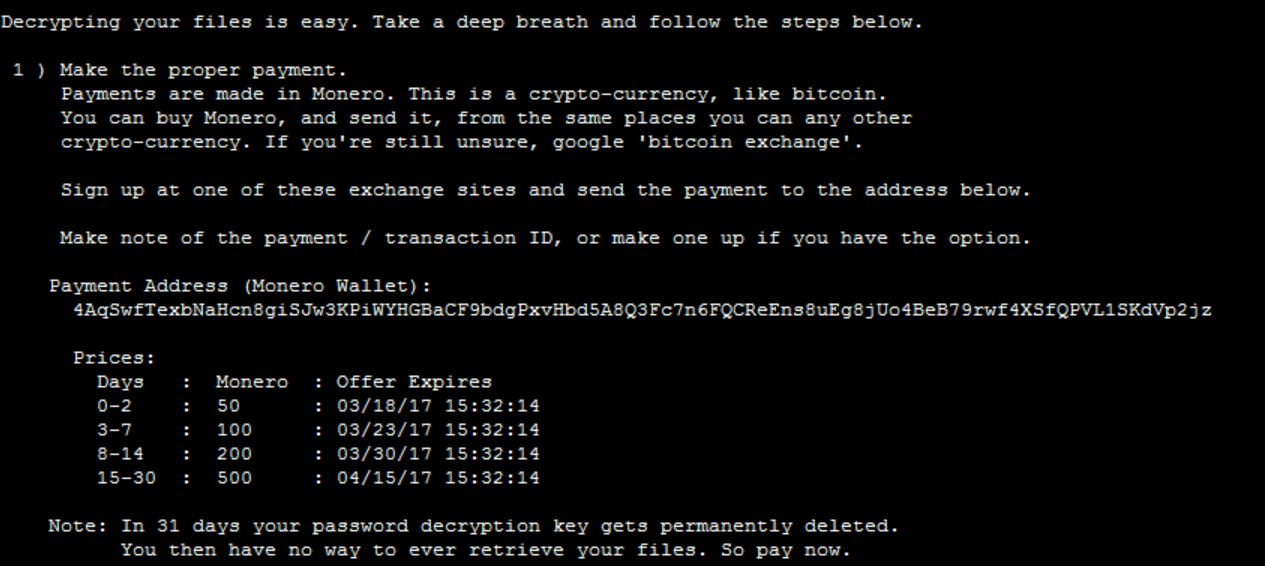
\includegraphics[trim={0 0 0 0},clip,width=0.9\textwidth]{stf-kirk-ransomware-virus-startrek-monero-payment-demands-ransom-instructions.png}
    \caption{Kirk ransomware that demands payment in Monero \protect\cite{monerokirk}.}
    \vspace{-1.5em}
    \label{pic:monerokirk}
\end{center}
    \end{figure}



\subsubsection{2) Scam portals}
\label{cha:scamportals}
As mentioned in the Section Wallets \ref{sec:wallets}, online wallets usage is a risky thing due to entrusting user's private keys to the third party. Users often choose them as they are not required to have any additional software. Due to this fact, there are more than ten domains that copy the design, functionality, and name of \url{mymonero.com} official online wallet with added code that steals the user's wallet data. Detailed list of domains is available at \url{https://www.reddit.com/r/Monero/wiki/avoid}.

Aside from direct scams, there are also services offering wallet services which have their codebase closed and store all wallet information. The best-known example of such service is \url{freewallet.org}, that is strongly criticized for closed source as well as funds that are reported as missing from user's accounts \cite{wijayamonero}.
\subsubsection{3) Crypto-jacking attack}
\label{cha:cryptojacking} 
Crypto-jacking a type of attack where the attacker delivers a malicious payload to the user's computer. Rather than rendering the device unusable either by blocking like ransomware, part of system resources is used for mining.

\begin{figure}[H]
\begin{center}

 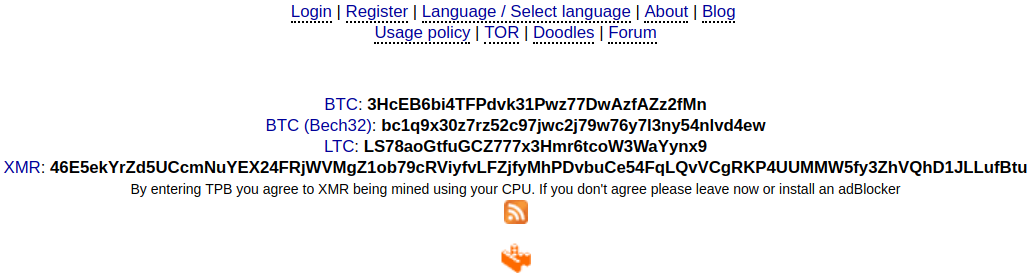
\includegraphics[trim={0 0 0 0},clip,width=0.95\textwidth]{cryptojacking.png}
    \caption{Some websites openly state that they mine Monero.}
    \label{pic:monerokirk}
\end{center}
    \end{figure}

Crypto-jacking is becoming more frequent than ransomware as it has proven that steady but low income is more profitable than one-time payment in the form of ransomware \cite{higbee2018role}.

\subsubsection{4) Black Ruby}
Interesting intersection of ransomware and crypto-jacking category is Black Ruby malware that combines features of both. First, it encrypts files on the target computer and then proceeds to mine Monero using XMRig at full CPU load \cite{blackruby2018}.

\vspace{-1em}
\section{Monero use case}
Aside from code quality and features, another important factor in cryptocurrency success are the ways how users can spend the funds. While numerous community around Monero that centers around Reddit \textit{/r/Monero} created \textit{/r/XMRtrader}, there are also projects that support Monero in day-to-day use like \url{https://xmr.to/}.

What is most noticeable tough, are darknet markets, that started to support payments by Monero. This results in the rather negative use case of the crypto as payments by Monero are not directly likable to one's wallet as described in the Section \ref{sec:ringsignatures}.

\begin{figure}[H]
\begin{center}

    \vspace{-0.8em}
 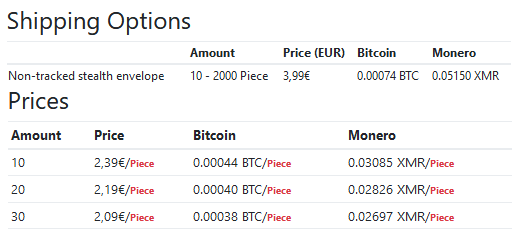
\includegraphics[trim={0 1.8cm 0 0},clip,width=0.71\textwidth]{Screenshot_360.png}
    \caption{Darknet market payment options.}
    \vspace{-1.5em}
    \label{pic:withoutresdrawable}
\end{center}
    \end{figure}


Although darknet markets may support Monero, a short inspection of Top 10 markets revealed that only 5 of them list Monero as the general way to pay. Rest of them are not forcing the sellers to use Monero. This results at about 40\% availability of Monero payment option on these type of markets.


\chapter{Monero User Research}
\label{cha:monerousersurvey}
The goal of this research is to gather information on end users behavior regarding Monero cryptocurrency with emphasis on key management and security practices. For this purpose, an online questionnaire was created. 

Specific survey design and research questions are based on Bitcoin security and privacy study, typical usage patterns of cryptocurrency users, online forums and Reddit communities centered around Monero as well as problematic areas regarding computer and data security in general \cite{krombholz2016other}.
\section{Research questions}
The survey was designed around seven question groups. Some of them were shown only if the participant chose the appropriate answer.
\begin{itemize}\itemsep0em
\item G01 - Introductory information
\item G02 - Monero usage
\item G03 - Monero key and coin management
\item G04 - Monero and malicious things
\item G05 - Monero recovery
\item G06 - Special question set for miners
\item G07 - Demographics
\end{itemize}
Following this pattern, four research questions were set:
\begin{itemize}\itemsep0em
\item R1: What are Monero's main use cases? How do participants perceive Monero's features? 
\item R2: What are participant's ways of wallet access and storage?
\item R3: What security incidents have affected users? How did they deal with them?
\item R4: In case of recovery, how did they recover their keys?
\end{itemize}
\section{Participants and survey's background}
The significant characteristic of Monero is its anonymity, and this feature is not taken by community lightly. Due to this fact, the survey was not hosted on third party servers, but instead on dedicated Virtual Private Server (VPS) running Lime Survey self-hosted software with HTTPS interface using signed Letsencrypt certificates \cite{certbot,limesurvey,letsencrypt}.

This means that data exchanged between participants and survey software stays only between these two parties, so Google or other big data company cannot analyze them. To allow extended anonymity features, Tor and proxy connections were allowed, but each participant had to solve the CAPTCHA before starting the survey.
\subsection{Methodology}
Data collection method was online only and was using the survey website software. Participants selection was based on opportunity sampling. Links for the research were shared among dedicated Reddit Monero community, Facebook Monero groups as well as Cryptocurrency forums.

To reduce nonresponse rate, participants were asked only to fill out parts that were significant for them, e.g., Monero recovery part stayed hidden in the form if the user selected that he/she had never made any recovery of the seed or wallet keys in the previous part. 

The data from the respondents were collected from 11.15.2018 to 01.27.2019. The complete survey is attached in the Appendix Figure \ref{monero-user-study-pdf}.

\section{Collected data}
Before entering the survey, each participant had to pass the bot test by entering the correct CAPTCHA, which resulted in 179 participants of the questionnaire in total. As for survey data cleansing, following measurements for valid dataset were taken:
\begin{enumerate}
\itemsep0em
\item Partially answered or unanswered questionnaires were not taken into account (67 out of 179). 
\item Respondents that filled out the survey in less than two minutes were discarded (1 out of 179).
\item Responses with more than 4 entries with the same IP were filtered (0 out of 179).
\begin{enumerate}
\itemsep0em
\item In total 7 responses were sent from duplicate IP addresses. The highest number of responses from a single IP was 3, which belonged to MIT University.
\end{enumerate}
\item Responses containing invalid answers, e.g., not using Monero or repeating the same answer pattern in multiple submissions (1 out of 179).
\end{enumerate}\vspace{-2.3em}
%\end{itemize}
\begin{center}
\begin{figure}[H]
\begin{tikzpicture}
\begin{axis}[
    xbar stacked,
    y dir = reverse,
    legend style={
    legend columns=2,
        at={(xticklabel cs:0.5)},
        anchor=north,
        draw=none
    },
    ytick=data,
    axis y line*=none,
    axis x line*=bottom, %bottom
    tick label style={font=\footnotesize},
    legend style={font=\footnotesize},
    label style={font=\footnotesize},
    xtick={0,100},
    width=.84\textwidth,
    bar width=6mm,
    xlabel={Time in ms},
    yticklabels={Filtered responses},
    xmin=0,
    xmax=100,
    area legend,
    xticklabel={\pgfmathparse{\tick}\pgfmathprintnumber{\pgfmathresult}\%},
    y=8mm,
   % enlarge y limits={abs=0.625},
]
\addplot[1,fill=1] coordinates {(62,0) };
%{(113,0) }; absolutni cisla, potrebuje to procenta
\addplot[3,fill=3] coordinates {(36,0) };
%{(67,0) };
\addplot[4,fill=4] coordinates {(1,0) };
%{(1,0) };
\addplot[6,fill=6] coordinates {(1,0) };
%{(1,0) };
\legend{Valid responses [113],Partially filled [67],Too fast [1],Invalid [1]
}
\coordinate (A) at (200,0);% ******** start of changes ************
\coordinate (B) at (300,8mm);
\end{axis}  
\node at (A) {test};
\node at (B) {test 2};% ********* end of changes **********
\end{tikzpicture}
\caption{Overview of respondents in the user survey dataset.}
\label{chart:price}\end{figure}\end{center}
\vspace{-3em}
Using \texttt{geoiplookup} package in Ubuntu on the filtered dataset, most of the responses were from USA (31 out of 113), followed by the Czech Republic (17 out of 113) and Germany (11 out of 113). Detailed list of countries with the corresponding number of responses is available in the Appendix Table \ref{table:countries}. 

\begin{figure}[H]
\begin{center}
\begin{tikzpicture}[]
\tikzstyle{every node}=[font=\scriptsize]
\pie []
    {27.4/USA,
15/Czech Republic,
9.7/Germany,
5.3/Canada,
4.4/Slovakia,
4.4/United Kingdom,
3.5/Belgium,
30.1/Others}
      
      
     \end{tikzpicture}
     \end{center}
      \caption{Responses sorted by country of origin based on IP location.}
      \label{chart:range}
\end{figure}

\iffalse
List of countries:
     31 US, United States
     17 CZ, Czech Republic
     11 DE, Germany
      6 CA, Canada
      5 SK, Slovakia
      5 GB, United Kingdom
      4 BE, Belgium
      3 RU, Russian Federation
      3 NL, Netherlands
      2 SI, Slovenia
      2 HK, Hong Kong
      2 FR, France
      2 FI, Finland
      2 BR, Brazil
      2 BG, Bulgaria
      2 AU, Australia
      1 UA, Ukraine
      1 TR, Turkey
      1 RS, Serbia
      1 RO, Romania
      1 PT, Portugal
      1 PL, Poland
      1 PH, Philippines
      1 NO, Norway
      1 MY, Malaysia
      1 MU, Mauritius
      1 IT, Italy
      1 GR, Greece
      1 ES, Spain
      1 AF, Afghanistan
\fi



\section{Results}
Next section is based on the final filtered dataset with 113 responses of people who voluntarily entered the research based on opportunity sampling.
\subsection{General information}
First, users were asked about their operating system preferences when accessing Monero. Majority of users tend to access Monero using Windows 58\% (65 out of 113) or Linux 60\% (68 out of 113). While accessing Monero from mobile Android OS 43\% (49 out of 113) is primarily used. As for the Apple ecosystem, MacOS combined with iOS was selected as used method of access only in 14\% (16 out of 113) occurences.


\begin{center}
\begin{figure}[H]
\begin{tikzpicture}
\begin{axis}[
    xbar stacked,
    y dir = reverse,
    legend style={
    legend columns=2,
        at={(xticklabel cs:0.5)},
        anchor=north,
        draw=none
    },
    ytick=data,
    axis y line*=none,
    axis x line*=bottom, %bottom
    tick label style={font=\footnotesize},
    legend style={font=\footnotesize},
    label style={font=\footnotesize},
    xtick={0,100},
    width=.95\textwidth,
    bar width=6mm,
    xlabel={Time in ms},
    yticklabels={Windows, Linux, MacOS, Android, 
		iOS},%{Official GUI, Official CLI, Other Desktop, Monerujo for Android, Freewallet on Android, Other Android wallet, Freewallet on iOS, Other iOS wallet, MyMonero Online wallet, XMRwallet Online, Other online wallet, Other},
    xmin=0,
    xmax=100,
    area legend,
    xticklabel={\pgfmathparse{\tick}\pgfmathprintnumber{\pgfmathresult}\%},
    y=8mm,
    enlarge y limits={abs=0.625},
]
\addplot[1,fill=1] coordinates {(58,0) (60,1)  (8,2) (43,3) (6,4)};
%{(113,0) }; absolutni cisla, potrebuje to procenta
\addplot[4,fill=4] coordinates {(42,0) (40,1) (92,2) (57,3) (94,4)};

\legend{Yes, No
}
\coordinate (A) at (25,0);% ******** start of changes ************
\coordinate (B) at (80,0);
\coordinate (C) at (25,-8mm);% ******** start of changes ************
\coordinate (D) at (80,-8mm);
\coordinate (E) at (3,-16mm);% ******** start of changes ************
\coordinate (F) at (45,-16mm);
\coordinate (G) at (25,-24mm);% ******** start of changes ************
\coordinate (H) at (80,-24mm);
\coordinate (CH) at (3,-32mm);% ******** start of changes ************
\coordinate (I) at (45,-32mm);
\end{axis}  
\node at (A) {65};
\node at (B) {48};% ********* end of changes **********
\node at (C) {68};
\node at (D) {45};% ********* end of changes **********
\node at (E) {9};
\node at (F) {104};% ********* end of changes **********
\node at (G) {49};
\node at (H) {64};% ********* end of changes **********
\node at (CH){7};
\node at (I) {106};% ********* end of changes **********
\end{tikzpicture}
\caption{Monero OS usage preferences.}
\label{chart:price}\end{figure}\end{center}

\subsubsection{Monero desktop application usage}
Desktop applications are used by 104 out of 113 users, making it the most frequent  means of accessing the wallet. As Monero Official application has no other direct competitors aside from web-based wallets, the majority of users 81\% (84 out of 104) use the official application with GUI, but there is also a notable part of the users in the dataset that use CLI as well 53\% (55 out of 104). Alternative desktop clients, that were sometimes misinterpreted as web apps, are used by only a few users cca 4\% (5 out of 104).

\begin{center}
\begin{figure}[H]
\begin{tikzpicture}
\begin{axis}[
    xbar stacked,
    y dir = reverse,
    legend style={
    legend columns=2,
        at={(xticklabel cs:0.5)},
        anchor=north,
        draw=none
    },
    ytick=data,
    axis y line*=none,
    axis x line*=bottom, %bottom
    tick label style={font=\footnotesize},
    legend style={font=\footnotesize},
    label style={font=\footnotesize},
    xtick={0,100},
    width=.86\textwidth,
    bar width=6mm,
    xlabel={Time in ms},
    yticklabels={Official GUI, Official CLI, Other Desktop},
    xmin=0,
    xmax=100,
    area legend,
    xticklabel={\pgfmathparse{\tick}\pgfmathprintnumber{\pgfmathresult}\%},
    y=8mm,
    enlarge y limits={abs=0.625},
]
\addplot[1,fill=1] coordinates {(81,0) (49,1)  (4,2) };
%{(113,0) }; absolutni cisla, potrebuje to procenta
\addplot[4,fill=4] coordinates {(19,0) (51,1) (96,2)};

\legend{Yes, No
}
\coordinate (A) at (50,0);% ******** start of changes ************
\coordinate (B) at (90,0);
\coordinate (C) at (25,-8mm);% ******** start of changes ************
\coordinate (D) at (80,-8mm);
\coordinate (E) at (2,-16mm);% ******** start of changes ************
\coordinate (F) at (50,-16mm);
\end{axis}  
\node at (A) {84};
\node at (B) {20};% ********* end of changes **********
\node at (C) {55};
\node at (D) {49};% ********* end of changes **********
\node at (E) {5};
\node at (F) {99};% ********* end of changes **********
\end{tikzpicture}
\caption{Desktop client software.}
\label{chart:price}\end{figure}\end{center}
\vspace{-2.25em}
\subsubsection{Monero Mobile app usage}
From 113 people that filled out the survey, 53 of them stated that they use either Android or iOS app for accessing their Monero wallet. Digging deeper, out of 49 Android users, Monerujo app is used by 92\% (45 out of 49) of them, followed by other Android wallets 14\% (7 out of 49). Freewallet on Android is only used by one user (2\%) in the dataset thus following the fact the community does not like closed source software with bad history as mentioned in the Chapter \ref{cha:scamportals}. 

\begin{center}
\begin{figure}[H]
\begin{tikzpicture}
\begin{axis}[
    xbar stacked,
    y dir = reverse,
    legend style={
    legend columns=2,
        at={(xticklabel cs:0.5)},
        anchor=north,
        draw=none
    },
    ytick=data,
    axis y line*=none,
    axis x line*=bottom, %bottom
    tick label style={font=\footnotesize},
    legend style={font=\footnotesize},
    label style={font=\footnotesize},
    xtick={0,100},
    width=.90\textwidth,
    bar width=6mm,
    xlabel={Time in ms},
    yticklabels={Monerujo, Freewallet, Other wallet},
    xmin=0,
    xmax=100,
    area legend,
    xticklabel={\pgfmathparse{\tick}\pgfmathprintnumber{\pgfmathresult}\%},
    y=8mm,
    enlarge y limits={abs=0.625},
]
\addplot[1,fill=1] coordinates {(92,1) (2,2) (14,3)};
%{(113,0) }; absolutni cisla, potrebuje to procenta
\addplot[4,fill=4] coordinates {(8,1) (98,2) (86,3)};

\legend{Yes, No
}
\coordinate (A) at (50,0);% ******** start of changes ************
\coordinate (B) at (95,0);
\coordinate (C) at (1,-8mm);% ******** start of changes ************
\coordinate (D) at (50,-8mm);
\coordinate (E) at (5,-16mm);% ******** start of changes ************
\coordinate (F) at (50,-16mm);
\end{axis}  
\node at (A) {45};
\node at (B) {4};% ********* end of changes **********
\node at (C) {1};
\node at (D) {48};% ********* end of changes **********
\node at (E) {7};
\node at (F) {42};% ********* end of changes **********
\end{tikzpicture}
\caption{Android client usage.}
\label{chart:price}\end{figure}\end{center}

iOS is used by 7 out of 113 users (please note that users could check usage of both platforms as can be visible from simply adding iOS and Android users and comparing it to the total number of mobile users). All of them (7) reported using the Cakewallet application. Following the Android pattern, one user also revealed usage of Freewallet app.



\begin{center}
\begin{figure}[H]
\begin{tikzpicture}
\begin{axis}[
    xbar stacked,
    y dir = reverse,
    legend style={
    legend columns=2,
        at={(xticklabel cs:0.5)},
        anchor=north,
        draw=none
    },
    ytick=data,
    axis y line*=none,
    axis x line*=bottom, %bottom
    tick label style={font=\footnotesize},
    legend style={font=\footnotesize},
    label style={font=\footnotesize},
    xtick={0,100},
    width=.90\textwidth,
    bar width=6mm,
    xlabel={Time in ms},
    yticklabels={CakeWallet,Freewallet, Other wallet, MyMonero Online wallet, XMRwallet Online, Other online wallet},
    xmin=0,
    xmax=100,
    area legend,
    xticklabel={\pgfmathparse{\tick}\pgfmathprintnumber{\pgfmathresult}\%},
    y=8mm,
    enlarge y limits={abs=0.625},
]
\addplot[1,fill=1] coordinates {(100,1) (14,2) (0,3)};
%{(113,0) }; absolutni cisla, potrebuje to procenta
\addplot[4,fill=4] coordinates {(0,1) (86,2) (100,3)};

\legend{Yes, No
}
\coordinate (A) at (50,0);% ******** start of changes ************
\coordinate (B) at (95,0);
\coordinate (C) at (7,-8mm);% ******** start of changes ************
\coordinate (D) at (50,-8mm);
\coordinate (E) at (5,-16mm);% ******** start of changes ************
\coordinate (F) at (50,-16mm);
\end{axis}  
\node at (A) {7};
\node at (B) {};% ********* end of changes **********
\node at (C) {1};
\node at (D) {6};% ********* end of changes **********
\node at (E) {};
\node at (F) {7};% ********* end of changes **********
\end{tikzpicture}
\caption{iOS client usage.}
\label{chart:price}\end{figure}\end{center}
\subsubsection{Online wallet services}
When asked about online wallet usage, only 24 people (out of 113) said that they use some sort of online service with MyMonero wallet being used the most 79\% (19 out of 24).

\begin{center}
\begin{figure}[H]
\begin{tikzpicture}
\begin{axis}[
    xbar stacked,
    y dir = reverse,
    legend style={
    legend columns=2,
        at={(xticklabel cs:0.5)},
        anchor=north,
        draw=none
    },
    ytick=data,
    axis y line*=none,
    axis x line*=bottom, %bottom
    tick label style={font=\footnotesize},
    legend style={font=\footnotesize},
    label style={font=\footnotesize},
    xtick={0,100},
    width=.90\textwidth,
    bar width=6mm,
    xlabel={Time in ms},
    yticklabels={MyMonero, XMRwallet, Other },
    xmin=0,
    xmax=100,
    area legend,
    xticklabel={\pgfmathparse{\tick}\pgfmathprintnumber{\pgfmathresult}\%},
    y=8mm,
    enlarge y limits={abs=0.625},
]
\addplot[1,fill=1] coordinates {(79,1) (16,2) (13,3)};
%{(113,0) }; absolutni cisla, potrebuje to procenta
\addplot[4,fill=4] coordinates {(21,1) (84,2) (87,3)};

\legend{Yes, No
}
\coordinate (A) at (50,0);% ******** start of changes ************
\coordinate (B) at (90,0);
\coordinate (C) at (7,-8mm);% ******** start of changes ************
\coordinate (D) at (50,-8mm);
\coordinate (E) at (7,-16mm);% ******** start of changes ************
\coordinate (F) at (50,-16mm);
\end{axis}  
\node at (A) {19};
\node at (B) {5};% ********* end of changes **********
\node at (C) {4};
\node at (D) {20};% ********* end of changes **********
\node at (E) {3};
\node at (F) {21};% ********* end of changes **********
\end{tikzpicture}
\caption{Online wallet usage.}
\label{chart:price}\end{figure}\end{center}

\subsubsection{Wallet software usage}
First part of the survey shows that userbase present in the dataset is more oriented towards open-source software in general (110 out of 113 use some form of open-source Monero client), but this is not limited to the usage of particular OS as there are 33\% (37 out of 113) of Windows only users, 35\% (40 out of 113) Linux only users and 25\% (28 out of 113) users of both OS. This discovery follows the information about Monero community as they prefer open source software (OSS) to closed source software (CSS) because they can not personally review for hidden features or unintentional bugs.

\begin{center}
\begin{figure}[H]
\begin{tikzpicture}
\begin{axis}[
    xbar stacked,
    y dir = reverse,
    legend style={
    legend columns=2,
        at={(xticklabel cs:0.5)},
        anchor=north,
        draw=none
    },
    ytick=data,
    axis y line*=none,
    axis x line*=bottom, %bottom
    tick label style={font=\footnotesize},
    legend style={font=\footnotesize},
    label style={font=\footnotesize},
    xtick={0,100},
    width=.84\textwidth,
    bar width=6mm,
    xlabel={Time in ms},
    yticklabels={Open-source usage, OS usage },
    xmin=0,
    xmax=100,
    area legend,
    xticklabel={\pgfmathparse{\tick}\pgfmathprintnumber{\pgfmathresult}\%},
    y=8mm,
    enlarge y limits={abs=0.625},
]
\addplot[1,fill=1] coordinates {(97,1) (0,2)};
%{(113,0) }; absolutni cisla, potrebuje to procenta
\addplot[4,fill=4] coordinates {(3,1) (0,2)};
\addplot[2,fill=2] coordinates {(0,1) (33,2)};
\addplot[3,fill=3] coordinates {(0,1) (35,2)};
\addplot[5,fill=5] coordinates {(0,1) (25,2)};
\addplot[6,fill=6] coordinates {(0,1) (7,2)};
\legend{Use at least 1 OSS, Use CSS, Windows, Linux, Both, Other}

\coordinate (A) at (50,0);% ******** start of changes ************
\coordinate (B) at (98.5,0);
\coordinate (C) at (18,-8mm);% ******** start of changes ************
\coordinate (D) at (50,-8mm);
\coordinate (E) at (80,-8mm);% ******** start of changes ************
\coordinate (F) at (97,-8mm);
\end{axis}  
\node at (A) {110};
\node at (B) {3};% ********* end of changes **********
\node at (C) {37};
\node at (D) {40};% ********* end of changes **********
\node at (E) {28};
\node at (F) {8};% ********* end of changes **********
\end{tikzpicture}
\caption{Open-source and OS preferences.}
\label{chart:price}\end{figure}\end{center}

\subsection{Monero usage}
When asked \enquote{\textit{What are your reasons to use Monero?}}, the majority of respondents in the dataset said that they use Monero or at least are interested in the topic because of the technology 88\% (99 out of 113), but also see it as an investment 73\% (83 out of 113). 

A significant portion of respondents also see Monero as a way of secret storage of value 74\% (84 out of 113) but not as much in the way of sending money 53\% (60 out of 113).

\begin{figure}[H]
\center
\begin{tabular}{>{\raggedright\arraybackslash}p{0.4\linewidth}%
   >{\centering\arraybackslash}p{0.25\linewidth}%
   >{\centering\arraybackslash}p{0.25\linewidth}%
  }
\textbf{Reason}          & \textbf{\% usage} & \textbf{Number of users (N=113)} \\
Investment               & 73 \%             & 83                \\
Technology               & 88 \%             & 99                \\
Fungibility              & 63 \%             & 71                \\
Hidden balance           & 74 \%             & 84                \\
Support Monero           & 65 \%             & 73                \\
Recommended by friend    & 04 \%              & 04                 \\
Secure storage of money  & 44 \%             & 50                \\
Secure transfer of funds & 53 \%             & 60                \\
To be paid in Monero     & 44 \%             & 50                \\
Other                    & 00 \%              & 00                
\end{tabular}
\caption{Reasons to use Monero.}
\label{table:monerousageresearch}
\end{figure}

This result is strongly affected by the way how participants were selected (self-selection) and from what sites they were informed about the survey (mainly Reddit Monero subreddits and Facebook Monero groups). The short overview of the preferences is shown in the Figure \ref{table:monerousageresearch} with the full text of the questions asked available in the Appendix Figure \ref{monero-user-study-pdf}.

\begin{center}
\begin{figure}[H]
\begin{tikzpicture}
\begin{axis}[
    xbar stacked,
    y dir = reverse,
    legend style={
    legend columns=2,
        at={(xticklabel cs:0.5)},
        anchor=north,
        draw=none
    },
    ytick=data,
    axis y line*=none,
    axis x line*=bottom, %bottom
    tick label style={font=\footnotesize},
    legend style={font=\footnotesize},
    label style={font=\footnotesize},
    xtick={0,100},
    width=.90\textwidth,
    bar width=6mm,
    xlabel={Time in ms},
    yticklabels={Transactions},
    xmin=0,
    xmax=100,
    area legend,
    xticklabel={\pgfmathparse{\tick}\pgfmathprintnumber{\pgfmathresult}\%},
    y=8mm,
    enlarge y limits={abs=0.625},
]
\addplot[1,fill=1] coordinates {(4,1)};
\addplot[2,fill=2] coordinates {(36,1)};
\addplot[4,fill=4] coordinates {(8,1)};
\addplot[3,fill=3] coordinates {(14,1)};
\addplot[5,fill=5] coordinates {((29,1)};
\addplot[7,fill=7] coordinates {(7,1)};

%{(113,0) }; absolutni cisla, potrebuje to procenta

\legend{Once a day, Once a month, Once a week, Once a year, Once every six months, Less than once a year
}
\coordinate (A) at (2,0);% ******** start of changes ************
\coordinate (B) at (22,0);
\coordinate (C) at (45,0);% ******** start of changes ************
\coordinate (D) at (55,0);
\coordinate (E) at (75,0);% ******** start of changes ************
\coordinate (F) at (95,0);
\end{axis}  
\node at (A) {5};
\node at (B) {39};% ********* end of changes **********
\node at (C) {9};
\node at (D) {15};% ********* end of changes **********
\node at (E) {31};
\node at (F) {8};% ********* end of changes **********
\end{tikzpicture}
\caption{Transaction frequency by Monero users.}
\label{chart:transactions}\end{figure}\end{center}

Transactions in the Monero network performed by respondents can be divided into two user groups, where the first group that can be described as active, those who make at least one transaction per month, 50\% (53 out of 107) and passive who are much less frequent 51\% (54 out of 107). Detailed overview of transactions frequency in the dataset is in the Figure \ref{chart:transactions}.


Following this question, respondents were asked if they hold onto their coins for a long time (often referred to as one being a HODLer). Majority of respondents 79\% (84 out of 106) said that they are, but this statement conflicts with transaction frequency. When comparing data of respondents that make a transaction at least every month, about 60\% (34 out of 57) think that they are HODLers, this contradicts the previously mentioned statement. 

\begin{figure}[H]
\center
%\begin{tabular}{cp{0.35\linewidth}rp{0.2\linewidth}r   p{0.35\linewidth} }
\begin{tabular}{>{\raggedright\arraybackslash}p{0.35\linewidth}%
   >{\centering\arraybackslash}p{0.2\linewidth}%
   >{\centering\arraybackslash}p{0.35\linewidth}%
  }
\textbf{Usage}          & \textbf{\% of users from total} & \textbf{N of users from total N=113} \\
Subscriptions           & 15\%             & 17                           \\
Restaurants             & 05\%              & 06                            \\
Donations               & 45\%             & 51                           \\
Art                     & 05\%              & 06                            \\
Electronics             & 18\%             & 20                           \\
Travelling              & 03\%              & 03                            \\
E-shops                 & 19\%             & 22                           \\
Darknet markets         & 18\%             & 20                           \\
Gambling sites          & 03\%              & 03                            \\
Drugs                   & 10\%             & 11                           \\
Illegal usecases        & 05\%              & 06                            \\
VPN services            & 35\%             & 31                           \\
Gift cards              & 04\%              & 04                            \\
Hosting and IT services & 22\%             & 25                           \\
Other                   & 00\%              & 00                           
\end{tabular}
\caption{Monero usage for payments.}
\label{table:moneropayusageresearch}
\end{figure}

Important usage factor of a currency is where its users can pay with it. Monero has already a known reputation between darknet markets, but its mainstream usage isn't something that is advertised as its feature. 

When asked about the payment options, many of the respondents 45\% (51 out of 113) selected that they use Monero as a way for donating other people, followed by paying for VPN services 35\% (31 out of 113). Although Monero features are considered ideal for black market use, only 5\% (6 out of 113) respondents revealed that they use Monero cryptocurrency in this way.%A detailed overview of payment types is available in the Appendix Figure \ref{table:moneropayusageresearch}.

Perception and the reality of anonymity in cryptocurrency is an important topic in the cryptocurrency environment \cite{amarasinghe2019survey}. Although Monero is private by default, additional precautions can be made to hide users activity from the third party like using Kovri or Tor. 

Among users in the dataset, Kovri 7\% (8 out of 113) or Tor 20\% (23 out of 113) is used by less than one third of the respondents in total as can be seen in the Figure \ref{table:moneropayusageresearch} .









\begin{center}
\begin{figure}[H]
\begin{tikzpicture}
\begin{axis}[
    xbar stacked,
    y dir = reverse,
    legend style={
    legend columns=2,
        at={(xticklabel cs:0.5)},
        anchor=north,
        draw=none
    },
    ytick=data,
    axis y line*=none,
    axis x line*=bottom, %bottom
    tick label style={font=\footnotesize},
    legend style={font=\footnotesize},
    label style={font=\footnotesize},
    xtick={0,100},
    width=.69\textwidth,
    bar width=6mm,
    xlabel={Time in ms},
    yticklabels={Transactions are anonymous, No one else can see the balance, Use Kovri to access Monero, Use Tor to access Monero},
    xmin=0,
    xmax=100,
    area legend,
    xticklabel={\pgfmathparse{\tick}\pgfmathprintnumber{\pgfmathresult}\%},
    y=8mm,
    enlarge y limits={abs=0.625},
]
\addplot[1,fill=1] coordinates {(88,1) (91,2) (7,3) (20,4)};
\addplot[4,fill=4] coordinates {(8,1) (7,2) (7,3) (3,4)};
\addplot[5,fill=5] coordinates {(2,1) (1,2) (79,3)(71,4)};
\addplot[6,fill=6] coordinates {(2,1) (1,2) (7,3) (6,4)};

%{(113,0) }; absolutni cisla, potrebuje to procenta

\legend{Yes, Uncertain, No, No response
}
\coordinate (A) at (50,0);% ******** start of changes ************
\coordinate (B) at (92,0);
\coordinate (C) at (50,-8mm);% ******** start of changes ************
\coordinate (D) at (94,-8mm);
\coordinate (E) at (4,-16mm);% ******** start of changes ************
\coordinate (F) at (11,-16mm);
\coordinate (G) at (50,-16mm);% ******** start of changes ************
\coordinate (H) at (10,-24mm);
\coordinate (CH) at (50,-24mm);% ******** start of changes ************

\end{axis}  
\node at (A) {99};
\node at (B) {10};% ********* end of changes **********
\node at (C) {103};
\node at (D) {8};% ********* end of changes **********
\node at (E) {8};
\node at (F) {7};% ********* end of changes **********
\node at (G) {90};% ********* end of changes **********
\node at (H) {23};% ********* end of changes **********
\node at (CH) {80};% ********* end of changes **********
\end{tikzpicture}
\caption{Perception of the Monero features.}
\label{chart:price}\end{figure}\end{center}
\pagebreak

\subsection{Monero key and coin management}
Apart from client software that is used for accessing and making transactions in Monero, wallet management is at least as important. Main reason is that users choice of wallet storage has a direct influence on who has access to the funds as explained along with the wallet types in the Chapter \ref{sec:wallets}.

\begin{center}
\begin{figure}[H]
\begin{tikzpicture}
\begin{axis}[
    xbar stacked,
    y dir = reverse,
    legend style={
    legend columns=2,
        at={(xticklabel cs:0.5)},
        anchor=north,
        draw=none
    },
    ytick=data,
    axis y line*=none,
    axis x line*=bottom, %bottom
    tick label style={font=\footnotesize},
    legend style={font=\footnotesize},
    label style={font=\footnotesize},
    xtick={0,100},
    width=.83\textwidth,
    bar width=6mm,
    xlabel={Time in ms},
    yticklabels={Hot wallet, Cold wallet, View-only wallet, Exchange wallet, Web wallet, Air-gapped wallet, Paper wallet, Hardware wallet},
    xmin=0,
    xmax=100,
    area legend,
    xticklabel={\pgfmathparse{\tick}\pgfmathprintnumber{\pgfmathresult}\%},
    y=8mm,
    enlarge y limits={abs=0.625},
]
\addplot[1,fill=1] coordinates {(60,1) (44,2) (10,3) (23,4) (15,5)(7,6)(25,6)(23,7)};
\addplot[4,fill=4] coordinates {(40,1) (56,2) (90,3) (77,4) (85,5) (93,6)(75,6)(77,7)};

%{(113,0) }; absolutni cisla, potrebuje to procenta

\legend{Yes, No
}
\coordinate (A) at (50,0);% ******** start of changes ************
\coordinate (B) at (80,0);
\coordinate (C) at (20,-8mm);% ******** start of changes ************
\coordinate (D) at (75,-8mm);
\coordinate (E) at (5,-16mm);% ******** start of changes ************
\coordinate (F) at (50,-16mm);
\coordinate (G) at (12,-24mm);% ******** start of changes ************
\coordinate (H) at (50,-24mm);
\coordinate (X) at (5,-32mm);% ******** start of changes ************
\coordinate (I) at (50,-32mm);
\coordinate (J) at (12,-40mm);% ******** start of changes ************
\coordinate (K) at (50,-40mm);
\coordinate (L) at (12,-48mm);% ******** start of changes ************
\coordinate (M) at (50,-48mm);
\end{axis}  
\node at (A) {68};
\node at (B) {45}; % ********* end of changes **********
\node at (C) {49};
\node at (D) {64};% ********* end of changes **********
\node at (E) {26};
\node at (F) {87};% ********* end of changes **********
\node at (G) {11};
\node at (H) {102};% ********* end of changes **********
\node at (X) {8};
\node at (I) {105};% ********* end of changes **********
\node at (J) {17};
\node at (K) {96};% ********* end of changes **********
\node at (L) {28};
\node at (M) {85};% ********* end of changes **********
\end{tikzpicture}
\caption{Wallet types usage in Monero.}
\label{chart:monerowalletsusagechart}\end{figure}\end{center}

\subsection{Monero recovery}
For further wallet protection, the majority of users also encrypt their wallet or the datastore on which the keys reside on 78\% (88 out of 113).

A slightly higher number of users admit backing up their wallet keys 89\% (101 out of 113) while a significant number of respondents had already needed to restore their wallet keys 44\% (50 out of 113). To complete the recovery statistics, 98\% (49 out of 50) were able to restore the keys from the backup media.

See the Figures \ref{chart:recoveryreason} and \ref{chart:recoverymethod} for visualization of wallet recovery reasons and restore methods.
\begin{center}
\begin{figure}[H]
\begin{tikzpicture}
\begin{axis}[
    xbar stacked,
    y dir = reverse,
    legend style={
    legend columns=2,
        at={(xticklabel cs:0.5)},
        anchor=north,
        draw=none
    },
    ytick=data,
    axis y line*=none,
    axis x line*=bottom, %bottom
    tick label style={font=\footnotesize},
    legend style={font=\footnotesize},
    label style={font=\footnotesize},
    xtick={0,100},
    width=.82\textwidth,
    bar width=6mm,
    xlabel={Time in ms},
    yticklabels={Recovery reason},
    xmin=0,
    xmax=100,
    area legend,
    xticklabel={\pgfmathparse{\tick}\pgfmathprintnumber{\pgfmathresult}\%},
    y=8mm,
    enlarge y limits={abs=0.625},
]
\addplot[1,fill=1] coordinates {(30,1)};
\addplot[4,fill=4] coordinates {(18,1)};
\addplot[5,fill=5] coordinates {(40,1)};
\addplot[6,fill=6] coordinates {(12,1)};

%{(113,0) }; absolutni cisla, potrebuje to procenta

\legend{Disk issue, Software issue, Device error, Not specified
}
\coordinate (A) at (16,0);% ******** start of changes ************
\coordinate (B) at (40,0);
\coordinate (C) at (68,0);% ******** start of changes ************
\coordinate (D) at (94,0);
\end{axis}  
\node at (A) {15};
\node at (B) {9};% ********* end of changes **********
\node at (C) {20};
\node at (D) {6};% ********* end of changes **********
\end{tikzpicture}
\caption{Reason for wallet recovery.}
\label{chart:recoveryreason}\end{figure}\end{center}
\vspace{-4em}
\begin{center}
\begin{figure}[H]
\begin{tikzpicture}
\begin{axis}[
    xbar stacked,
    y dir = reverse,
    legend style={
    legend columns=3,
        at={(xticklabel cs:0.5)},
        anchor=north,
        draw=none
    },
    ytick=data,
    axis y line*=none,
    axis x line*=bottom, %bottom
    tick label style={font=\footnotesize},
    legend style={font=\footnotesize},
    label style={font=\footnotesize},
    xtick={0,100},
    width=.82\textwidth,
    bar width=6mm,
    xlabel={Time in ms},
    yticklabels={Restore method},
    xmin=0,
    xmax=100,
    area legend,
    xticklabel={\pgfmathparse{\tick}\pgfmathprintnumber{\pgfmathresult}\%},
    y=8mm,
    enlarge y limits={abs=0.625},
]
\addplot[1,fill=1] coordinates {(18,1)};
\addplot[2,fill=2] coordinates {(4,1)};
\addplot[4,fill=4] coordinates {(10,1)};
\addplot[5,fill=5] coordinates {(51,1)};
\addplot[6,fill=6] coordinates {(17,1)};
%{(113,0) }; absolutni cisla, potrebuje to procenta

\legend{Hard drive, Cloud storage, Flash drive, Paper media, Mnemonic seed
}
\coordinate (A) at (10,0);% ******** start of changes ************
\coordinate (B) at (20,0);
\coordinate (C) at (27,0);% ******** start of changes ************
\coordinate (D) at (55,0);
\coordinate (E) at (92,0);
\end{axis}  
\node at (A) {9};
\node at (B) {2};% ********* end of changes **********
\node at (C) {5};
\node at (D) {26};% ********* end of changes **********
\node at (E) {8};% ********* end of changes **********
\end{tikzpicture}
\caption{Method used for wallet recovery.}
\label{chart:recoverymethod}\end{figure}\end{center}
\vspace{-4em}
\subsection{Monero and malicious software}
\label{cha:maliciousminingresearch}
This part was answered only by those respondents that selected Yes (15 out of 113) when asked whether they have ever been affected by malicious software that used Monero in some way.

The primary cause of problems was mining malware (8) or some form of mining script (7). The main affected platform was running Windows (10), and malware was recognized mainly by slow system response (7) and high CPU usage (11).

When trying to compare the security of individual wallet types, one of the important factors that determine its usability and security is wallet recovery rate. To compare the hot and cold wallet approach using the Chi-Square test, the following hypothesis was set:
\begin{itemize}\itemsep0em
\item H0: There is no difference between the hot and cold wallet and their recovery rate.
\item H1: There is a difference between the hot and cold wallet and their recovery rate.
\end{itemize}
The table with extracted values is in the Table \ref{table:user-chi}. The chi-square statistic is 0.489. The p-value is .484356. The result is not significant at p < .05. Therefore it means that the data provide little or no evidence that the null hypothesis is false. 

\begin{figure}[H]
\centering

\begin{tabular}{llll}
                       & \textbf{Hot wallet}            & \textbf{Cold wallet}           & \textbf{Row Totals} \\
\textbf{Recovery yes}  & 36  (34.16)  {[}0.10{]} & 23  (24.84)  {[}0.14{]} & 59                  \\
\textbf{Recovery no}   & 30  (31.84)  {[}0.11{]} & 25  (23.16)  {[}0.15{]} & 55                  \\
\textbf{Column Totals} & 66                      & 48                      & 114
\end{tabular}


\captionof{table}{Contingency Table for wallet types and recovery.}
\label{table:user-chi}
\end{figure}



\subsection{Demographics}
Survey participants were mainly males 44\% (50 out of 113), females 2\% (2 out of 113) represented only a small portion of the dataset, and some of the participants did not disclose their gender 54\% (61 out of 113). Most respondents in the dataset were from the age groups 25-34 29\% (33 out of 113). 
\vspace{-1em}
\begin{center}
\begin{figure}[H]
\begin{tikzpicture}
\begin{axis}[
    xbar stacked,
    y dir = reverse,
    legend style={
    legend columns=3,
        at={(xticklabel cs:0.5)},
        anchor=north,
        draw=none
    },
    ytick=data,
    axis y line*=none,
    axis x line*=bottom, %bottom
    tick label style={font=\footnotesize},
    legend style={font=\footnotesize},
    label style={font=\footnotesize},
    xtick={0,100},
    width=.82\textwidth,
    bar width=6mm,
    xlabel={Time in ms},
    yticklabels={Respondents age},
    xmin=0,
    xmax=100,
    area legend,
    xticklabel={\pgfmathparse{\tick}\pgfmathprintnumber{\pgfmathresult}\%},
    y=8mm,
    enlarge y limits={abs=0.625},
]
\addplot[1,fill=1] coordinates {(33,1)};
\addplot[2,fill=2] coordinates {(41,1)};
\addplot[3,fill=3] coordinates {(18,1)};
\addplot[4,fill=4] coordinates {(3,1)};
\addplot[5,fill=5] coordinates {(1,1)};
\addplot[7,fill=7] coordinates {(1,1)};
\addplot[6,fill=6] coordinates {(3,1)};
%{(113,0) }; absolutni cisla, potrebuje to procenta

\legend{18-24,25-34,35-44,45-54,55-64,65-74,75+
}
\coordinate (A) at (17,0);% ******** start of changes ************
\coordinate (B) at (55,0);
\coordinate (C) at (85,0);% ******** start of changes ************
\end{axis}  
\node at (A) {37};
\node at (B) {47};% ********* end of changes **********
\node at (C) {21};
\end{tikzpicture}
\caption{Age groups in the dataset.}
\label{chart:agegroupsuserresearch}\end{figure}\end{center}
\vspace{-3.3em}
\begin{center}
\begin{figure}[H]
\begin{tikzpicture}
\begin{axis}[
    xbar stacked,
    y dir = reverse,
    legend style={
    legend columns=2,
        at={(xticklabel cs:0.5)},
        anchor=north,
        draw=none
    },
    ytick=data,
    axis y line*=none,
    axis x line*=bottom, %bottom
    tick label style={font=\footnotesize},
    legend style={font=\footnotesize},
    label style={font=\footnotesize},
    xtick={0,100},
    width=.82\textwidth,
    bar width=6mm,
    xlabel={Time in ms},
    yticklabels={Level of education},
    xmin=0,
    xmax=100,
    area legend,
    xticklabel={\pgfmathparse{\tick}\pgfmathprintnumber{\pgfmathresult}\%},
    y=8mm,
    enlarge y limits={abs=0.625},
]
\addplot[1,fill=1] coordinates {(9,1)};
\addplot[2,fill=2] coordinates {(29,1)};
\addplot[4,fill=4] coordinates {(52,1)};
\addplot[6,fill=6] coordinates {(10,1)};
%{(113,0) }; absolutni cisla, potrebuje to procenta

\legend{Primary education, Secondary education, Tertiary education, Not specified
}
\coordinate (A) at (4,0);% ******** start of changes ************
\coordinate (B) at (25,0);
\coordinate (C) at (70,0);% ******** start of changes ************
\coordinate (D) at (95,0);
\end{axis}  
\node at (A) {10};
\node at (B) {33};% ********* end of changes **********
\node at (C) {59};
\node at (D) {11};
\end{tikzpicture}
\caption{Highest achieved level of education.}
\label{chart:educationleveluserresearch}\end{figure}\end{center}
\vspace{-4.2em}
\begin{center}
\begin{figure}[H]
\begin{tikzpicture}
\begin{axis}[
    xbar stacked,
    y dir = reverse,
    legend style={
    legend columns=3,
        at={(xticklabel cs:0.5)},
        anchor=north,
        draw=none
    },
    ytick=data,
    axis y line*=none,
    axis x line*=bottom, %bottom
    tick label style={font=\footnotesize},
    legend style={font=\footnotesize},
    label style={font=\footnotesize},
    xtick={0,100},
    width=.82\textwidth,
    bar width=6mm,
    xlabel={Time in ms},
    yticklabels={Work in industry},
    xmin=0,
    xmax=100,
    area legend,
    xticklabel={\pgfmathparse{\tick}\pgfmathprintnumber{\pgfmathresult}\%},
    y=8mm,
    enlarge y limits={abs=0.625},
]
\addplot[1,fill=1] coordinates {(65,1)};
\addplot[2,fill=2] coordinates {(33,1)};
\addplot[4,fill=4] coordinates {(2,1)};
%{(113,0) }; absolutni cisla, potrebuje to procenta

\legend{IT industry, Other industry, Not specified
}
\coordinate (A) at (35,0);% ******** start of changes ************
\coordinate (B) at (84,0);
\coordinate (C) at (99,0);% ******** start of changes ************
\end{axis}  
\node at (A) {74};
\node at (B) {37};% ********* end of changes **********
\node at (C) {2};
\end{tikzpicture}
\caption{Respondents and IT industry.}
\label{chart:itindustryuserresearch}\end{figure}\end{center}

\chapter{Monero Usage and Storage Best Practices}
Ease of use is one of the critical aspects of every cryptocurrency and although Monero can offer a wide range of privacy features it has to be usable and user-friendly to be used by a substantial margin of people. Usability in Monero is a long-term topic that sparks discussion \cite{monerolang2018}.

Following scenarios represent secure and easy to use instructions for a new Monero user, based on results from Monero user research in the Chapter \ref{cha:monerousersurvey}.

\section{Generating the keys and accessing the wallet}
The first challenge for Monero users is generating key pairs and accessing the wallet. This process varies from the user's platform of choice and used wallet software. As the choice of client wallet software is important for Monero users in terms of user experience and security, the following Sections are dedicated to available wallet software. %TODO je to better oproti původnímu As the choice of client wallet software is fundamental for users Monero regarding user experience and security standpoint, following sections are dedicated to available  wallet software.
\subsection{Windows and Linux platform}
The official client offers CLI and GUI wallet management and is available at \url{https://getmonero.org/downloads/}. Using this client users can generate wallet keys. Created keys are after generation saved directly into the memory of the device unless specified otherwise. 
\begin{figure}[H]
\begin{center}
  %  \vspace{-0.8em}
 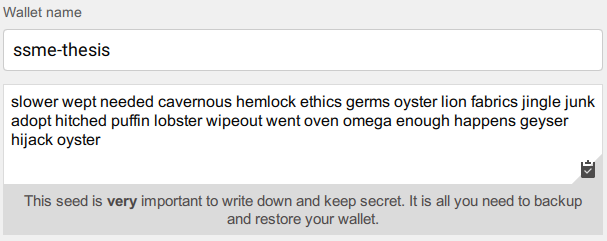
\includegraphics[trim={0 0 0 0},clip,width=0.85\textwidth]{Screenshot_4.png}
    \caption{GUI wallet generation.}
  %  \vspace{-1.5em}
    \label{pic:guigenerator}
\end{center}
    \end{figure}

\begin{figure}[H]
\begin{center}
\begin{lstlisting}
.\monero-wallet-cli.exe
Monero Lithium Luna (v0.12.3.0-release)
Logging to C:\...\monero-wallet-cli.log
Specify wallet file name (e.g., MyWallet). If the wallet 
file is not present, it will be created.
Wallet file name (or Ctrl-C to exit): ssme-thesis
No wallet found with that name. Confirm creation of new 
wallet named: ssme-thesis
(Y/Yes/N/No): Y
Generating new wallet...
\end{lstlisting}
\caption{CLI wallet generation.}
    \label{pic:cligenerator}
\end{center}
    \end{figure}
    \vspace{-1em}
Security of this task depends on the origin of the software, delivery chain trust, and the users' operating system. Monero CLI and GUI binaries can be edited, and the app itself does not call any internal checking to alert the user of the unauthorized change. 

Code injection was successfully tested on GUI binary of the official Monero wallet as seen in the Figure \ref{pic:codeinjectiongui}. Although SHA256 hash is provided on the website, the user is not specifically instructed to check the hashes of the downloaded software with tools like PowerShell using \texttt{Get-FileHash ./monero-wallet-gui.exe | Format-List} command \cite{pialphapialphagammaiotaacutealphanunualpharhoovarsigma2016study}. GPG-signed list of the hashes is available on the website although there are no instructions on how to verify PGP signature itself.
    \vspace{-1em}
\begin{figure}[H]
\begin{center}
\begin{lstlisting}
Algorithm : SHA256
Hash      : AF9324151909AC7B9BC6D622210EADFBAE5E66...
Path      : ./monero-wallet-gui-original.exe

Algorithm : SHA256
Hash      : DF4EC49E088284ECC78DBBD8B9CEFF00A78085...
Path      : ./monero-wallet-gui-injected.exe
\end{lstlisting}
\caption{Checksum change after code injeciton.}
    \label{pic:codeinjectiongui}
\end{center}
    \end{figure}


%  Wallet key generation process is shown on examples in the Figures \ref{pic:cligenerator} and \ref{pic:guigenerator}. \\

There are also alternative approaches to key generation like an offline JavaScript based monero-wallet-generator that is available at \url{github.com/moneromooo-monero/monero-wallet-generator}.

\subsection{Hardware wallet}

Hardware way is considered to be in the development, but Monero compatible devices like Ledger Nano S are already on the market. The way how keys are generated in hardware wallets varies on firmware included in each device. 

In general, the wallet is required to have Monero app installed from vendors app catalog. Keys are generated on the hardware device within the app itself, and the user can only export private view key from the device to view the balance in full CLI/GUI client.

This way, the user has private spend key always on the device, and the client PC has only private view key. To sign a transaction, the user has to confirm the transaction on the device itself meaning the hardware wallet will sign the transaction and then sends it to the Monero client. By this, in case of a security breach on the host computer, there is no Monero to steal.

\subsection{Wallet software for mobile devices}

Monero has wallet software available for Android as well as the iOS platform. Community recommends to use the open source ones for both platforms, as their codebase is published on GitHub and everyone can inspect the code. Another common fact for the recommended solutions is that the keypairs for the wallet are stored exclusively on the user's device and restore can be done without third-party technical support.

\textbf{Monerojuro} is an open source Android wallet application that is available on Google Play as well as APK release at Github. By this, users can install the application from the Google Play directly, manually download the APK or compile it from source code themselves. Wallet keys storage is based on the device only, and the application encourages users to back up their seed \cite{xmrwalletgithub}.

\textbf{Monero Wallet} is an application released by Freewallet.org that provides Monero wallets for both Android and iOS. Regarding overall usability, this application is easier for an average user as it does not present any cryptocurrency wallet terms as key, seed, etc. The user is instead instructed to create a Freewallet account which acts as a wallet \cite{freewallet}. 

By this, the user does not need to save the seed, wallet keys or make any backups as key management is completely on the side of the service provider, Freewallet.org. This fact is often emphasized in Monero community as the user that does not control the keys does not control the wallet. Also, the source code is not publicly available for the community to review.

\textbf{Cake Wallet} represents open source Monero wallet for iOS that provides wallet generation and local key pair storage with remote node connection and synchronization \cite{cakewalletgithub}.

Guideline for secure wallet access is described in the Chapter \ref{sec:wallettypes}. 

\begin{figure}[H]
\begin{center}
\vspace{-0.75em}
 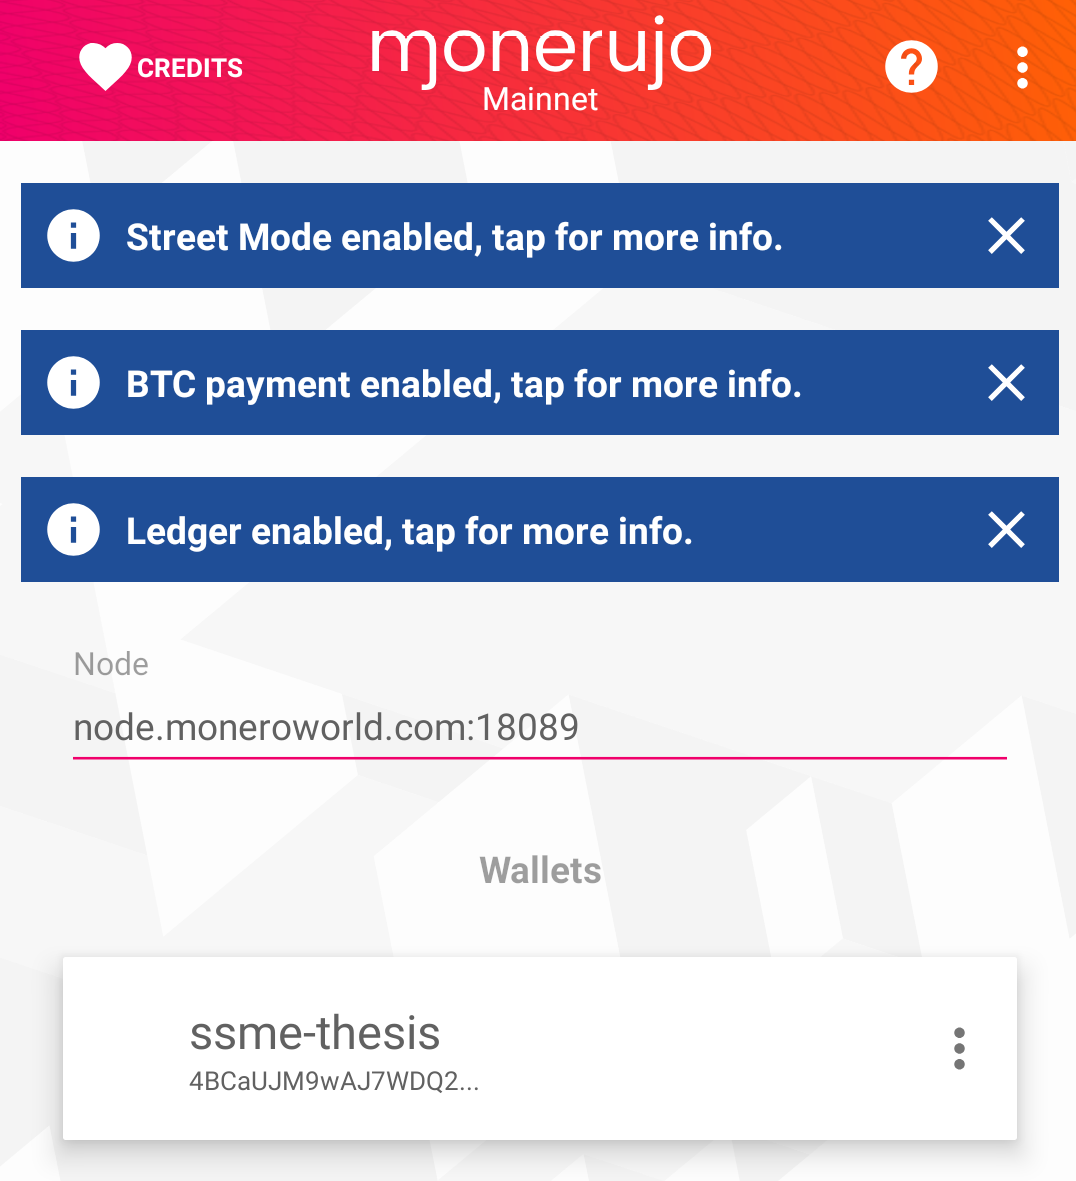
\includegraphics[trim={0 1.8cm 0 0},clip,width=0.4\textwidth]{Screenshot_1542566492.png}
    \caption{Monerujo for Android.}
    \vspace{-1.5em}
    \label{pic:withoutresdrawable}
\end{center}
    \end{figure}
 \vspace{-0.9em}
\begin{figure}[H]
\centering\begin{tabular}{p{0.2\linewidth}p{0.15\linewidth}p{0.1\linewidth}p{0.4\linewidth}}
\textbf{Name}         & \textbf{Platform}      & \textbf{Source}        & \textbf{Wallet keys management} \\
Monerojuro    & Android       & Open Source   & Keypair is stored locally.  User has complete control.                      \\
Monero \linebreak Wallet & Android  iOS & Closed Source & Keypair in cloud storage. No control over keys. \\
Cake Wallet   & iOS           & Open Source   & Keypair is stored locally.  User has complete control.                           
\end{tabular}
\captionof{table}{List of avaiable wallets for mobile platforms.}
\label{table:monero-mobile}
\end{figure}


\section{Secure storage system}
Wallet keys are everything when it comes to cryptocurrency usage. Who has the keys, controls the wallet and can view or transfer the balance to another address. If a user loses wallet keys, Monero wallet can still be recovered using mnemonic seed that should be saved on another storage medium. 

This Section describes possible ways of backing-up wallet keys. Primary storage media security is compared in the Figure \ref{fig:walletstorage}.
\subsubsection{Data characteristics}
As described in the Section \ref{sec:wallets}, Monero wallet consists of an encrypted \texttt{wallet.keys} file that contains private spend and view keys. Size of this file is less than a few kilobytes. 

Another type of data that is presented to the user is mnemonic seed. Seed can be used for recovery when wallet file is lost and consists of 25 words with the last one being used for checksum. 

In total, Monero wallet requires less than 8 kilobytes for key and seed storage. This results in minimal space requirements for backup storage media.

\subsubsection{Backup strategy}
Best practice for backups that isn't too demanding on the user side is the 3-2-1 strategy that is considered in the industry as a bare minimum for keeping the data safe \cite{storage2012data}. 
\begin{itemize}
\itemsep0em
\item 3 means having at least 3 copies of your data in total.
\item 2 of them are local but stored on different media types.
\begin{itemize}
\itemsep0em
\item This can be represented as a combination of SSD and tape.
\end{itemize}
\item 1 is an offsite, geographically different location.
\begin{itemize}
\itemsep0em
\item E.g., in the next building, a different facility, another city.
\end{itemize}
\end{itemize}
In short, this means when your building with external drive burns down and your notebook gets cryptolocker on the same day, you still have your data safe as you have them in the offsite location.

\begin{figure}[H]
\centering
\begin{tabular}{p{0.1\linewidth}p{0.4\linewidth}p{0.20\linewidth}p{0.15\linewidth}}
\textbf{Media type} & \textbf{Available key security}                                    & \textbf{Usage}                                   & \textbf{Average pricing}      \\
HDD, SSD            & File and volume encryption, can be automated.                       & Manual transfer from master to external media.    & 20-40 USD                              \\
Optical media       & File-based encryption before creating the media, manual process.            & For each copy of data, new disc has to be used.   & \textless{}1 USD                       \\
Tape                & Hardware assisted drive encryption, software-based encryption.       & Specialised backup tape software.                & 4500 USD (tape + drive) \\
NAS                 & File-based encryption on the client side using encryption software or NAS feature. & Manual or automatic transfer to a network share.    & 200-400 USD                            \\
Cloud drive       & File-based encryption on the client side using encryption software. & Clientside software that syncs files from master & Free or paid 10 USD monthly                      \\
Paper               & Depends on printout content and physical storage properties.        & Hiding a sheet of paper.                          & \textless{}1 USD                       \\

\end{tabular}


\captionof{table}{Common storage methods with security features.}
\label{table:secure-storage}
\end{figure}

Data that users need to backup are not changing in the day to day usage, but only when the user creates a new or an additional wallet. Meaning that backing up the wallet does not need to be made frequently unlike other user data that are changed frequently, e.g., documents. Verification, on the other hand, is more important as not only users should back up the data, they should also be able to restore them. For ease of use, users can verify the integrity of the backup by actually recovering the wallet from the backup media.

\subsubsection{Recommended scheme}
Following cost effectivity of individual media types together with common backup strategy:
\begin{itemize}
\itemsep0em
\item Total number of copies of data: 5
\item The primary data source is on the client device with wallet software. This source is then copied downstream to backup media.
\item All copies of the data should be encrypted using file-level encryption regardless of the security of the device, e.g., by a popular open-source tool like VeraCrypt.
\item Local copy
\begin{itemize}
\itemsep0em
\item Located on disk with full volume encryption, e.g., by BitLocker.
\item Paper backup in a secure container at a hidden place.
\end{itemize}
\item Offsite copy
\begin{itemize}
\itemsep0em
\item Located on the flash drive with full volume encryption.
\item Located on the DVD as an encrypted file.
\end{itemize}
\end{itemize}

\subsubsection{Secure Monero usage portal}
As a result of this Chapter and Monero user research in the Chapter \ref{cha:monerousersurvey}, all recommendations for secure Monero usage are compiled within one website \url{https://ownercz.github.io/ssme-thesis}.

\iffalse
\begin{figure}[H]
\begin{center}

    
 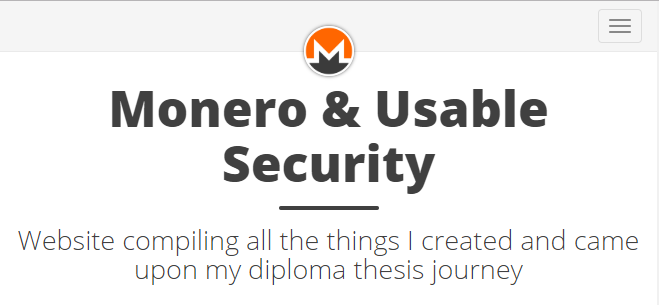
\includegraphics[trim={0 0 5px 1px},clip,width=1\textwidth]{Screenshot_7.png}
    \caption{Monero secure usage portal.}

    \label{pic:moneroweb}
\end{center}
    \end{figure}
    \fi

\chapter{Obtaining Monero and Running the Network}
\label{cha:obtaining}
Monero mining is a process done by miners to verify transactions on the network and add them to the blockchain together in the form of a block. This results for them in a reward in the form of new coins that are emitted as a reward for block solving.

Network speed is mainly determined by the average time between individual blocks. %This results in transaction process that takes up to 130s (transaction request \textless 1s, network broadcast \textless 5s and transaction processing time as a time between submission and next mined block \textless 120 seconds). 
This results in the transaction process that takes up to 130s (request =\textless 1s, broadcast =\textless 5s and max. time between blocks =\textless 120 seconds).  The transaction process is shown in the Figure \ref{pict:network-processing}.

\begin{figure}[H]
\center
\definecolor{ao(english)}{rgb}{0.0, 0.5, 0.0}
\definecolor{azure(colorwheel)}{rgb}{0.0, 0.5, 1.0}
\definecolor{darkorange}{rgb}{1.0, 0.55, 0.0}
\tikzstyle{decision} = [diamond, draw, fill=blue!20,
    text width=4.5em, text badly centered, node distance=2.5cm, inner sep=0pt]
\tikzstyle{userA} = [rectangle, draw, fill=ao(english)!20,
    text width=5em, text centered, rounded corners, minimum height=4em]
\tikzstyle{userB} = [rectangle, draw, fill=azure(colorwheel)!20,
    text width=5em, text centered, rounded corners, minimum height=4em]
\tikzstyle{userC} = [rectangle, draw, fill=darkorange!20,
    text width=5em, text centered, rounded corners, minimum height=4em]
\tikzstyle{lineuserA} = [draw, very thick, color=ao(english)!80, -latex']

\tikzstyle{lineuserB} = [draw, very thick, color=azure(colorwheel)!80, -latex']
\tikzstyle{lineuserC} = [draw, very thick, color=darkorange!80, -latex']
\tikzstyle{cloud} = [draw, ellipse,fill=red!20, node distance=2.5cm,
    minimum height=2em]

\begin{tikzpicture}[scale=2, node distance = 2cm, auto]
\shorthandoff{-}
    % Place nodes
    \node [userA,text width=5cm,minimum width=5cm] (userA1) {\parbox{5cm}{\centering Transaction request generated by the client \texttt{transfer ADDRESS AMOUNT}}};
    \node [userB, right of=userA1, node distance=6cm, text width=5cm,minimum width=5cm] (userB1)    {\parbox{5cm}{\centering Request broadcast to network nodes, shown \texttt{show\TextUnderscore{}transfers pool} }};
    
    \node [below of=userA1,node distance=2.5cm,text width=5cm,minimum width=5cm, draw=none] (userA2){};
    \node [userB, below of=userB1, node distance=2.5cm,text width=5cm,minimum width=5cm] (userB2)    {\parbox{5cm}{\centering Transaction is added to the block waiting to be mined.}};
    
    \node [userC, below of=userA2,node distance=2.5cm,text width=5cm,minimum width=5cm] (userA3)  {\parbox{5cm}{\centering Miners are verifying transactions in the pending block.}}; %, in cli called multisig wallet password
    \node [userB, below of=userB2, node distance=2.5cm,text width=5cm,minimum width=5cm] (userB3)    {\parbox{5cm}{\centering Every 2 minutes new Monero block is mined and added to the blockchain.}}; %, in cli called multisig wallet password
    
    
    \node [userC, below of=userA3,node distance=2.5cm,text width=5cm,minimum width=5cm] (userA4) {\parbox{5cm}{\centering Miners are rewarded by block reward.}};
    \node [userB, below of=userB3, node distance=2.5cm,text width=5cm,minimum width=5cm] (userB4)    {\parbox{5cm}{\centering Receiving party's wallet becomes aware of the transaction.}};
        
   % \node [block, below of=init, node distance=2.5cm,text width=3cm,minimum width=3cm] (identify) {\parbox{3cm}{\centering Repackaging by reseller}};
%    \node [block, below of=identify, node distance=2.5cm,text width=3cm,minimum width=3cm] (evaluate) {\parbox{3cm}{\centering HW wallet bought by enduser}};
 %   \node [cloud, left of=identify, node distance=5cm] (update) {\parbox{3cm}{\centering Malicious scratchpad with seed  }};
  %  \node [block, below of=evaluate, node distance=2.5cm,text width=3cm,minimum width=3cm] (attacker) {\parbox{3cm}{\centering Attacker's database of wallets}};
    % Draw edges
    \path [lineuserC] (userA3) -- (userB3);
   % \path [lineuserA] (userA2) -- (userA4);
    \path [lineuserB] (userB1) -- (userB2);
    \path [lineuserB] (userB2) -- (userB3);
    \path [lineuserB] (userB3) -- (userB4);
    \path [lineuserB] (userB3) to[in=14,out=210,looseness=0] (userA4);
        \path [lineuserA] (userA1) to[in=-165,out=-15,looseness=0]  (userB1);
        \path [lineuserB] (userB1) to[in=15,out=165,looseness=0]   (userA1);
   % \path [line] (identify) -- (evaluate);
   %\path [line] (expert) -- (init);
  % \path [lineuserA] (userA2) |- (userB2);
\end{tikzpicture}
\caption{Monero network processing.}
\label{pict:network-processing}
\end{figure}
\newpage
\section{Mining nodes}
As was mentioned at the beginning of the Chapter \ref{cha:obtaining}, mining is the main reason for transaction processing in Monero network, and as the mining process has rewards for successfully solving the block, this encourages many different entities to mine.\iffalse
Since Bitcoin started to gain popularity, mining has divided into five categories, that are described in the following Sections:  

\begin{itemize}\topsep0em\parskip0em\parsep0em
\begin{minipage}{0.4\linewidth}
\item Mining in pools \ref{cha:poolmining}
\item Solo mining \ref{cha:solomining}
\item Web mining \ref{cha:webmining}
\end{minipage}
\begin{minipage}{0.4\linewidth}
\item Botnet mining \ref{cha:botnetmining}
\item Cloud mining \ref{cha:cloudmining}
\end{minipage}
\end{itemize}
\fi
\subsubsection{Mining in pools}
\label{cha:poolmining}
Very often, miners combine their computational resources into one of the pools on the network. Due to the higher total hash rate, there is a greater chance of solving the block thus gaining the reward of newly emitted coins. After solving each block, the reward is distributed equally to miners connected to the pool according to PPS (per-per-share) or PPLNS (per-per-last-number-of-shares) system \cite{tarasiewicz2015cryptocurrencies}.

As of 09.29.2018 total hash rate of the network was 577.72 Mh/s (100\%), in known pools 530.79 Mh/s (91.88\%) and unknown part of the network 46.93 Mh/s (8.12\%). Unknown part represents either pools that are not listed or solo miners on the network.


\begin{figure}[H]
\begin{center}
\begin{tikzpicture}[]
\tikzstyle{every node}=[font=\footnotesize]
\pie []
    {26.79/nanopool.org,
      19.17/minexmr.com,
      18.02/supportxmr.com,
      5.69/miningpoolhub.com,
      22.21/other pools,
      8.12/unknown}
      
      
     \end{tikzpicture}
     \end{center}
      \caption{Hash rate distribution in Monero network.}
      \label{chart:range}

\end{figure}
\subsubsection{Solo mining}
\label{cha:solomining}
Represents "all or nothing" approach when it comes to the rewarding system. As solo miner's hash rate has to compete against all other solo miners as well as big pools, the chance of solving the block is rather small \cite{cong2018decentralized}.

On the other side, when solo miner solves the block successfully, the whole block reward is assigned to the mining address. With high-end, multiple GPU setup, the miner can achieve about 3.2 Kh/s; this would mean chance about 0.46 \% of gaining the block reward. 

\subsubsection{Web mining}
\label{cha:webmining}
CryptoNight algorithm mining stands out above others in the way how cryptocurrency can be mined. For Monero there are JavaScript-based miners like CoinHive available, that results in individual websites embedding this script and mining using the visitor's resources. 

This can result up to 300 hashes per second for users with powerful CPUs and is a viable alternative to advertisements when visitors spend more than 10 minutes on the website \cite{papadopoulos2018truth}. Typical examples of this approach are warez websites offering free online movies and torrent trackers.
% Web mining: https://arxiv.org/pdf/1806.01994.pdf
\subsubsection{Botnet mining}
\label{cha:botnetmining}
Using other peoples resources for mining, often also called crypto jacking (a more broad term for hidden cryptocurrency mining without users approval), have become increasingly popular in Monero. As the cryptocurrency provides privacy features as well as a wide range of mining software that is available for every major platform.

In the current cloud era of computing, this represents vast problems for both service providers and their customers. Providers experience increased power consumption, cooling requirements, customers, on the other hand, are required to pay more for consumed system resources \cite{tahir2017mining}.

\subsubsection{Cloud mining}
\label{cha:cloudmining}
\definecolor{ao(english)}{rgb}{0.0, 0.5, 0.0}
\definecolor{azure(colorwheel)}{rgb}{0.0, 0.5, 1.0}
\definecolor{darkorange}{rgb}{1.0, 0.55, 0.0}
Represents managed services by specialists that offer mining power using cloud service providers. Due to managed service providers (MSP) markup, this way of mining is not as profitable and not recommended among Monero community in general. \\Arrows indicate flow of the resources:\\ \textcolor{ao(english)} {Payment for service}; \textcolor{azure(colorwheel)}{Payment for compute time}; \textcolor{darkorange}{Delivered hashrate}

\begin{figure}[H]
\center
\tikzstyle{decision} = [diamond, draw, fill=blue!20,
    text width=4.5em, text badly centered, node distance=2.5cm, inner sep=0pt]
\tikzstyle{userA} = [rectangle, draw, fill=ao(english)!20,
    text width=5em, text centered, rounded corners, minimum height=4em]
\tikzstyle{userB} = [rectangle, draw, fill=azure(colorwheel)!20,
    text width=5em, text centered, rounded corners, minimum height=4em]
\tikzstyle{userC} = [rectangle, draw, fill=darkorange!20,
    text width=5em, text centered, rounded corners, minimum height=4em]
\tikzstyle{lineuserA} = [draw, very thick, color=ao(english)!80, -latex']

\tikzstyle{lineuserB} = [draw, very thick, color=azure(colorwheel)!80, -latex']
\tikzstyle{lineuserC} = [draw, very thick, color=darkorange!80, -latex']
\tikzstyle{cloud} = [draw, ellipse,fill=red!20, node distance=2.5cm,
    minimum height=2em]

\begin{tikzpicture}[scale=2, node distance = 0.4cm, auto]
\shorthandoff{-}
    % Place nodes
    \node [userA,text width=2cm,minimum width=2cm] (userA1) {\parbox{2cm}{\centering Hashrate buyer}};
    \node [userB, right of=userA1, node distance=4cm, text width=2cm,minimum width=2cm] (userB1)    {\parbox{2cm}{\centering MSP }};
    \node [userC, right of=userB1, node distance=4cm, text width=2cm,minimum width=2cm] (userC1)    {\parbox{2cm}{\centering Datacentre }};
        
   % \node [block, below of=init, node distance=2.5cm,text width=3cm,minimum width=3cm] (identify) {\parbox{3cm}{\centering Repackaging by reseller}};
%    \node [block, below of=identify, node distance=2.5cm,text width=3cm,minimum width=3cm] (evaluate) {\parbox{3cm}{\centering HW wallet bought by enduser}};
 %   \node [cloud, left of=identify, node distance=5cm] (update) {\parbox{3cm}{\centering Malicious scratchpad with seed  }};
  %  \node [block, below of=evaluate, node distance=2.5cm,text width=3cm,minimum width=3cm] (attacker) {\parbox{3cm}{\centering Attacker's database of wallets}};
    % Draw edges
        \path [lineuserA] (userA1) -- (userB1);
        %\path [lineuserB] (userB1) to[in=15,out=165,looseness=0]   (userA1);
        \path [lineuserB] (userB1) --  (userC1);
        \path [lineuserC] (userC1) to[in=35,out=145,looseness=1]   (userA1);
   % \path [line] (identify) -- (evaluate);
   %\path [line] (expert) -- (init);
  % \path [lineuserA] (userA2) |- (userB2);
\end{tikzpicture}
\caption{Monero network processing.}
\label{pict:network-processing}
\end{figure}

\section{Mining software}
\subsubsection{Official}
Can be obtained at the official web of the Monero cryptocurrency project at \url{https://getmonero.org/downloads/}. This is an official wallet software that includes solo mining client and cannot be used for pool mining.

\subsubsection{Community-driven}
\label{cha:miningsoftware}
Is a category that incorporates open-source mining software projects that have source code published on the Github. Mostly used are:

\begin{itemize}\itemsep0em
\item XMR Stak 
\begin{itemize}\itemsep0em \item Consolidates CPU, AMD and Nvidia GPU mining under one multiplatform application with integrated webserver and autoconfiguration capability. \item URL: \url{https://github.com/fireice-uk/xmr-stak} \end{itemize}
\setlength\itemsep{1em}
\item XMRig 
\setlength\itemsep{0em}
\begin{itemize}\itemsep0em \item Three separately released miners with autoconfiguration GPU and CPU capability. \item AMD: \url{https://github.com/xmrig/xmrig-amd} 
 \item Nvidia: \url{https://github.com/xmrig/xmrig-nvidia} \item CPU: \url{https://github.com/xmrig/xmrig} \end{itemize}
\item CCminer - Nvidia CUDA miner
\begin{itemize}\itemsep0em \item URL: \url{https://github.com/tpruvot/ccminer/} \end{itemize}
\end{itemize}

\begin{figure}[H]
\begin{center}

    \vspace{-0.8em}
 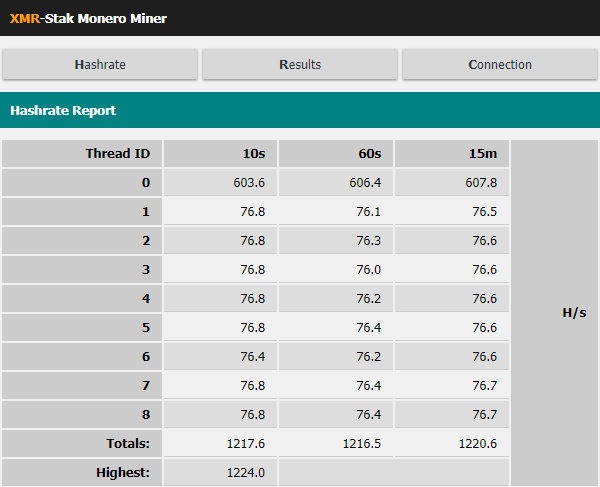
\includegraphics[trim={0 0 0 0},clip,width=0.85\textwidth]{Screenshot_9.png}
    \caption{XMR-Stak web interface.}
    \vspace{-1.5em}
    \label{pic:withoutresdrawable}
\end{center}
    \end{figure}
    
\subsubsection{Proprietary}
Having closed source code that community cannot inspect, mining software of this category has less reputation compared to the community-driven. This is caused mainly by the fact that the exact produced hash rate and client reported hash rate differed in the past at least regarding the MinerGate miner available at \url{https://minergate.com/downloads/gui} .

\section{Mining malware }
\vspace{-0.2em}
As Monero algorithm is designed to be memory demanding algorithm, it is suitable to mine it using both CPU and GPU as mining software offers support for both hardware components as mentioned in the Section \ref{cha:miningsoftware}. 

The fact that Monero can be effectively CPU mined means for malware miners much easier way how to gain any profit from infected computer as they do not need to have any specific GPU drivers or features implemented. Because of this, they are easier to deploy on a wide range of devices \cite{le2018swimming}.
\vspace{-0.6em}
\subsubsection{Monero position in the malware world}
When malicious software developer considers the cryptocurrency technology to build on, cryptocurrency features are one of the most important aspects that drive this decision.

In the case of Monero, its features are as much important for its users as for the malware developers. The main reason for using Monero is that it offers private features as well as support for mining on almost every device available \cite{eskandari2018first}.

Thanks to its features and active development, Monero is one of the most active cryptocurrencies that are used in the malware world with more than 57M USD already mined. As of 2019, Monero is identified to have the most active malware campaigns per cryptocurrency, followed by Bitcoin and zCash \cite{konoth2019malicious}.
\vspace{-0.6em}
\subsubsection{Types of malware miners}
Main categories of malware miners are derived from the way how the unwanted software is delivered to the target device. Most common ways of ingestion are:
\begin{itemize}
\itemsep0em
\item Website with JavaScript miner software, also known as Cryptojacking as mentioned in the Figure \ref{cha:cryptojacking}. 
\item Exploiting vulnerabilities in the operating system or application software.
\item Bundled in legitimate software.
\end{itemize}
%\subsubsection{Unwanted mining in SOHO envionment}
%\ref{cha:maliciousminingresearch}
%\subsubsection{Unwanted mining in large scale}


%\subsection{Systems administrators perspective}
%kitty https://www.incapsula.com/blog/crypto-me0wing-attacks-kitty-cashes-in-on-monero.html
%\subsection{Regular users}

\iffalse
\section{XMR obtaining comparison}
\begin{figure}[H]
\center
\begin{tabular}{p{0.2\linewidth}p{0.16\linewidth}p{0.16\linewidth}p{0.16\linewidth}p{0.16\linewidth}p{0.16\linewidth}}
\textbf{Mining type} & \textbf{Security} & \textbf{Depenence} & \textbf{Payout} & \textbf{Avaiability} & \textbf{Profitability} \\
Pool mining          &                   &                    &                 &                      &                        \\
Solo mining          &                   &                    &                 &                      &                        \\
Web mining           &                   &                    &                 &                      &                        \\
Botnet mining        &                   &                    &                 &                      &                        \\
Cloud mining         &                   &                    &                 &                      &                       
\end{tabular}
\caption{Monero network processing.}
\label{pict:network-processing}
\end{figure}
\fi
\chapter{Monero Miners Research}
%tento výzkum jsem nenašel, takže říct, že tam nic dalšího není napsat to tam
%zobrazování voleb pro multiple choice randomizovat
% total hardware dát pryč a místo toho jen hashrate OK
%obtain software > official github OK
%2x mám incident OK
%pooly podle abecedy OK
%vypustit verzi windows OK
%other u linux os OK
%mining os dodat OK
% škola > dodá Vlasta info
% místo interested in modern technologies >> eearly adopter OK
% privacy aspect vygooglit části
The goal of this research is to gather information on people who run mining cryptocurrency software and map their behavior regarding system administration with the emphasis on security practices. For this purpose, an online questionnaire was created and is avaiable in the Appendix Figure \ref{monero-user-study-pdf}. 

To the best of my knowledge, this is the first work that studies cryptocurrency miners. Specific research questions are based on cryptocurrency mining setup patterns, used software and problematic areas regarding computer and data security in general. 

\section{Research questions}
The survey was designed around seven question groups. Some of them were shown only if the participant chose the appropriate answer.
\begin{itemize}\itemsep0em
\item G01 - Introductory information
\item G02 - Mining setup
\item G03 - Mining software
\item G04 - Pool choice
\item G05 - Windows platform
\item G06 - Linux platform
\item G07 - Demographics
\end{itemize}
Following this pattern, five research questions were set:
\begin{itemize}\itemsep0em
\item R1: Who are Monero miners in general? What are their typical mining setups? 
\item R2: Which types of software do participants use as operating systems, management, and mining tools?
\item R3: What security and update policies miners follow? 
\item R4: Do miners suffer from security incidents like compromised mining operation? How do they deal with them?
\item R5: What are the factors that affect pool choice?
\end{itemize}
\section{Participants and survey's background}
As mentioned in the Chapter \ref{cha:monerousersurvey}, the survey was not hosted on third party servers, but instead on dedicated VPS running Lime Survey self-hosted software with HTTPS interface using signed Letsencrypt certificates.

This means that data exchanged between participants and survey software stays only between these two parties, so Google or other big data companies cannot analyze them. To allow extended privacy features, Tor and proxy connections were allowed, but each participant had to solve the CAPTCHA before starting the survey.
%\vspace{-0.7em}
\subsection{Methodology}
Data collection method was online only and was using the survey website software. Participants selection was based on opportunity sampling, links for the research were shared among dedicated Reddit Monero community, Facebook Mining groups as well as Cryptocurrency forums. This form was distributed together with the Monero User Research survey in mentioned mining communities.

To reduce nonresponse rate, participants were asked only to fill out parts that were significant for them, e.g., Windows OS part stayed hidden in the form if the user selected that he/she used Linux OS only. 

The data from the respondents were collected from 11.15.2018 to 01.27.2019. The complete survey is attached in the Appendix Figure \ref{monero-miners-study-pdf}.
%\vspace{-0.7em}
\section{Collected data}
Before entering the survey, each participant had to pass the bot test by entering the correct CAPTCHA, which resulted in 323 participants of the questionnaire in total. As for survey data cleansing, following measurements for valid dataset were taken:
\begin{enumerate}
%\itemsep-0.2em
\item Partially answered or unanswered questionnaires were not taken into account (261 out of 323). 
\item Respondents that filled out the survey in less than two minutes were discarded (0 out of 323).
\newpage
\item Responses with more than four entries with the same IP were filtered (0 out of 323).
\item Responses containing invalid answers, e.g., not using Monero or repeating the same answer pattern in multiple submissions (2 out of 323).
\end{enumerate}
\vspace{-2em}
%\end{itemize}
\begin{center}
\begin{figure}[H]
\begin{tikzpicture}
\begin{axis}[
    xbar stacked,
    y dir = reverse,
    legend style={
    legend columns=2,
        at={(xticklabel cs:0.5)},
        anchor=north,
        draw=none
    },
    ytick=data,
    axis y line*=none,
    axis x line*=bottom, %bottom
    tick label style={font=\footnotesize},
    legend style={font=\footnotesize},
    label style={font=\footnotesize},
    xtick={0,100},
    width=.84\textwidth,
    bar width=6mm,
    xlabel={Time in ms},
    yticklabels={Filtered responses},
    xmin=0,
    xmax=100,
    area legend,
    xticklabel={\pgfmathparse{\tick}\pgfmathprintnumber{\pgfmathresult}\%},
    y=8mm,
   % enlarge y limits={abs=0.625},
]
\addplot[1,fill=1] coordinates {(19,0) };
%{(113,0) }; absolutni cisla, potrebuje to procenta
\addplot[3,fill=3] coordinates {(80,0) };
%{(67,0) };
\addplot[4,fill=4] coordinates {(0,0) };
%{(1,0) };
\addplot[6,fill=6] coordinates {(1,0) };
%{(1,0) };
\legend{Valid responses [60],Partially filled [261],Too fast [0],Invalid [2]
}
\coordinate (A) at (200,0);% ******** start of changes ************
\coordinate (B) at (300,8mm);
\end{axis}  
\node at (A) {test};
\node at (B) {test 2};% ********* end of changes **********
\end{tikzpicture}
\caption{Overview of respondents in the miners survey dataset.}
\label{chart:price}\end{figure}\end{center}

Using \texttt{geoiplookup} package in Ubuntu on the filtered dataset, most of the responses were from the USA (10 out of 60) as well as from the Czech Republic (10 out of 60) followed by Germany (6 out of 60). Detailed list of countries with the corresponding number of responses is available in the Appendix Table \ref{table:countriesminers}. 
\vspace{-1em}
\begin{figure}[H]
\begin{center}
\begin{tikzpicture}[]
\tikzstyle{every node}=[font=\scriptsize]
\pie []
    {17/USA,
17/Czech Republic,
10/Germany,
5/Russian Federation,
5/Portugal,
5/Canada,
41/Others}
      
      
     \end{tikzpicture}
     \end{center}
      \caption{Responses sorted by country of origin based on IP location.}
      \label{chart:range}
\end{figure}





\section{Results}
Upcoming pages are based on the final filtered dataset with 60 responses of people who voluntarily entered the research based on opportunity sampling.
\vspace{-0.5em}
\subsubsection{General information}
When asked about the motivation for mining Monero, two-thirds of the respondents 67\% (40  out of 60) think about Monero as an investment, but also as a way to gain some profit from mining cryptocurrencies 62\% (37 out of 60). 

Although Monero is not considered to be more profitable to mine by the majority in the dataset 77\% (46 out of 60), almost half of the miners 47\% (28 out of 60) favor this cryptocurrency due to its mining characteristics CPU minable and the fact that they directly help to secure the network by mining 60\% (36 out of 60). 

Note that the reasons for mining Monero are biased by the way the respondents in the dataset were selected. In general, there would be a higher percentage of the cryptocurrency miners that care only for the profitability rather than cryptocurrency features \cite{al2014investigating}.
    \vspace{-1em}
\subsubsection{Mining setup}
Gathering information about mining setups was designed as a multiple-choice question where every choice was described in detail as illustrated in the Figure \ref{pic:miningquestion}. 

\begin{figure}[H]
\begin{center}

 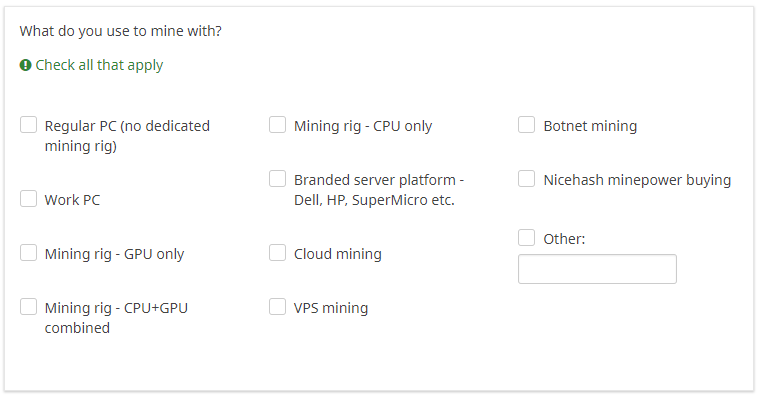
\includegraphics[trim={0.5cm 1.7cm 0.5cm 0.5cm},clip,width=0.85\textwidth]{Screenshot_31.png}
    \caption{Mining setup question.}
    \label{pic:miningquestion}
\end{center}
    \end{figure}

Even through dataset cleansing, from the final 60 respondents, 15 of them chose both \textit{Regular PC only} and \textit{Mining rig} option. Therefore, only 45 respondents are taken into account in this part.
    

\begin{center}
\begin{figure}[H]
\begin{tikzpicture}
\begin{axis}[
    xbar stacked,
    y dir = reverse,
    legend style={
    legend columns=2,
        at={(xticklabel cs:0.5)},
        anchor=north,
        draw=none
    },
    ytick=data,
    axis y line*=none,
    axis x line*=bottom, %bottom
    tick label style={font=\footnotesize},
    legend style={font=\footnotesize},
    label style={font=\footnotesize},
    xtick={0,100},
    width=.84\textwidth,
    bar width=6mm,
    xlabel={Time in ms},
    yticklabels={Mining hardware},
    xmin=0,
    xmax=100,
    area legend,
    xticklabel={\pgfmathparse{\tick}\pgfmathprintnumber{\pgfmathresult}\%},
    y=8mm,
   % enlarge y limits={abs=0.625},
]
\addplot[1,fill=1] coordinates {(38,0) };
%{(113,0) }; absolutni cisla, potrebuje to procenta
\addplot[2,fill=2] coordinates {(27,0) };
%{(67,0) };
\addplot[4,fill=4] coordinates {(4,0) };
%{(1,0) };
\addplot[6,fill=6] coordinates {(31,0) };
\legend{GPU only [17],CPU and GPU [12], CPU only [2], No response [14]
}
\end{axis}  
\end{tikzpicture}
\caption{Mining types comparison.}
\label{chart:miningtype}\end{figure}\end{center}    
    
When asked about mining setup, the majority of the miners mine on their PC 33\% (15 out of 45) or also on mining rig 69\% (31 out of 45), but there is also a small portion of miners 18\% (8 out of 45) that use their employer's hardware and electricity to run their mining operation. On the other side, only two of the respondents mentioned mining on a VPS instance and no one selected cloud mining or botnet mining as their way to mine Monero.

\begin{center}
\begin{figure}[H]
\begin{tikzpicture}
\begin{axis}[
    xbar stacked,
    y dir = reverse,
    legend style={
    legend columns=2,
        at={(xticklabel cs:0.5)},
        anchor=north,
        draw=none
    },
    ytick=data,
    axis y line*=none,
    axis x line*=bottom, %bottom
    tick label style={font=\footnotesize},
    legend style={font=\footnotesize},
    label style={font=\footnotesize},
    xtick={0,100},
    width=.79\textwidth,
    bar width=6mm,
    xlabel={Time in ms},
    yticklabels={Mine in own property, Own rig setup, Windows mining, Linux mining, 
		Cleaning, Updates regular, UPS},%{Official GUI, Official CLI, Other Desktop, Monerujo for Android, Freewallet on Android, Other Android wallet, Freewallet on iOS, Other iOS wallet, MyMonero Online wallet, XMRwallet Online, Other online wallet, Other},
    xmin=0,
    xmax=100,
    area legend,
    xticklabel={\pgfmathparse{\tick}\pgfmathprintnumber{\pgfmathresult}\%},
    y=8mm,
    enlarge y limits={abs=0.625},
]
\addplot[1,fill=1] coordinates {(87,0) (93,1)  (65,2) (55,3)};
%{(113,0) }; absolutni cisla, potrebuje to procenta
\addplot[4,fill=4] coordinates {(13,0) (7,1) (35,2) (45,3)};

\legend{Yes, No
}
\coordinate (A) at (50,0);% ******** start of changes ************
\coordinate (B) at (93,0);
\coordinate (C) at (50,-8mm);% ******** start of changes ************
\coordinate (D) at (96,-8mm);
\coordinate (E) at (40,-16mm);% ******** start of changes ************
\coordinate (F) at (80,-16mm);
\coordinate (G) at (40,-24mm);% ******** start of changes ************
\coordinate (H) at (80,-24mm);
\end{axis}  
\node at (A) {52};
\node at (B) {8};% ********* end of changes **********
\node at (C) {56};
\node at (D) {4};% ********* end of changes **********
\node at (E) {39};
\node at (F) {21};% ********* end of changes **********
\node at (G) {33};
\node at (H) {27};% ********* end of changes **********
\end{tikzpicture}
\caption{Mining setup properties.}
\label{chart:miningproperties}\end{figure}\end{center}
97\% (58 out of 60) of respondents shared their current hashrate with median hashrate value being 4.4Kh/s. This hashrate represents a typical setup with 5 high-performance  GPUs (AMD RX 480 8GB with 800-850h/s) or 7 high-performance CPUs (AMD Ryzen 7 1700 with 600-650h/s).

Majority of miners mine in their property 87\% (52 out of 60) and set up their mining rigs 93\% (56 out of 60). The operating system is not dominant nor on the Windows side 65\% (39 out of 60) nor the Linux part 55\% (33 out of 60) described in the Figure \ref{chart:miningproperties}. This is mainly because of multiplatformity of mining software and availability of guides for mining setups. 
\begin{center}
\begin{figure}[H]
\begin{tikzpicture}
\begin{axis}[
    xbar stacked,
    y dir = reverse,
    legend style={
    legend columns=2,
        at={(xticklabel cs:0.5)},
        anchor=north,
        draw=none
    },
    ytick=data,
    axis y line*=none,
    axis x line*=bottom, %bottom
    tick label style={font=\footnotesize},
    legend style={font=\footnotesize},
    label style={font=\footnotesize},
    xtick={0,100},
    width=.86\textwidth,
    bar width=6mm,
    xlabel={Time in ms},
    yticklabels={Cleaning, Regular updates, UPS},%{Official GUI, Official CLI, Other Desktop, Monerujo for Android, Freewallet on Android, Other Android wallet, Freewallet on iOS, Other iOS wallet, MyMonero Online wallet, XMRwallet Online, Other online wallet, Other},
    xmin=0,
    xmax=100,
    area legend,
    xticklabel={\pgfmathparse{\tick}\pgfmathprintnumber{\pgfmathresult}\%},
    y=8mm,
    enlarge y limits={abs=0.625},
]
\addplot[1,fill=1] coordinates {(51,1) (70,2) (23,3)};
%{(113,0) }; absolutni cisla, potrebuje to procenta
\addplot[4,fill=4] coordinates { (49,1) (30,2) (77,3)};

\legend{Yes, No
}
\coordinate (A) at (30,0);% ******** start of changes ************
\coordinate (B) at (80,0);
\coordinate (C) at (50,-8mm);% ******** start of changes ************
\coordinate (D) at (80,-8mm);
\coordinate (E) at (10,-16mm);% ******** start of changes ************
\coordinate (F) at (50,-16mm);
\end{axis}  
\node at (A) {31};
\node at (B) {29};% ********* end of changes **********
\node at (C) {42};
\node at (D) {18};% ********* end of changes **********
\node at (E) {14};
\node at (F) {46};% ********* end of changes **********
\end{tikzpicture}
\caption{Mining setup preferences.}
\label{chart:mininghabits}\end{figure}\end{center}
\vspace{-2em}
Miners generally tend to update their rigs 70\% (42 out of 60) as well as clean them 52\% (31 out of 60) but refrain from additional infrastructure costs like buying a UPS 23\% (14 out of 60) as shown in the Figure \ref{chart:mininghabits}.

\subsubsection{Mining software}
The choice of mining software impacts mining profitability as well as the number of shares that are donated to the developer (if any). 

As described in the Chapter \ref{cha:miningsoftware}, most popular mining software falls into open source with great moderation regarding code updates from the crypto community in general. This follows results from the dataset where XMR Stak project, that is the most active on Github, is also the most preferred way to run the mining operation 78\% (47 out of 60 miners).
\begin{center}
\begin{figure}[H]
\begin{tikzpicture}
\begin{axis}[
    xbar stacked,
    y dir = reverse,
    legend style={
    legend columns=2,
        at={(xticklabel cs:0.5)},
        anchor=north,
        draw=none
    },
    ytick=data,
    axis y line*=none,
    axis x line*=bottom, %bottom
    tick label style={font=\footnotesize},
    legend style={font=\footnotesize},
    label style={font=\footnotesize},
    xtick={0,100},
    width=.86\textwidth,
    bar width=6mm,
    xlabel={Time in ms},
    yticklabels={ XMR Stak, XMRig, Wallet software, MinerGate},%{Official GUI, Official CLI, Other Desktop, Monerujo for Android, Freewallet on Android, Other Android wallet, Freewallet on iOS, Other iOS wallet, MyMonero Online wallet, XMRwallet Online, Other online wallet, Other},
    xmin=0,
    xmax=100,
    area legend,
    xticklabel={\pgfmathparse{\tick}\pgfmathprintnumber{\pgfmathresult}\%},
    y=8mm,
    enlarge y limits={abs=0.625},
]
\addplot[1,fill=1] coordinates {(78,1) (30,2) (11,3) (3,4)};
%{(113,0) }; absolutni cisla, potrebuje to procenta
\addplot[4,fill=4] coordinates { (22,1) (70,2) (89,3) (97,4)};

\legend{Yes, No
}
\coordinate (A) at (40,0);% ******** start of changes ************
\coordinate (B) at (90,0);
\coordinate (C) at (15,-8mm);% ******** start of changes ************
\coordinate (D) at (60,-8mm);
\coordinate (E) at (5,-16mm);% ******** start of changes ************
\coordinate (F) at (50,-16mm);
\coordinate (G) at (1.5,-24mm);% ******** start of changes ************
\coordinate (H) at (50,-24mm);
\end{axis}  
\node at (A) {47};
\node at (B) {13};% ********* end of changes **********
\node at (C) {18};
\node at (D) {42};% ********* end of changes **********
\node at (E) {7};
\node at (F) {53};% ********* end of changes ********** 
\node at (G) {2};
\node at (H) {58};% ********* end of changes ********** 
\end{tikzpicture}
\caption{Mining software preference.}
\label{chart:mininghabits}\end{figure}\end{center}
\vspace{-2em}
XMRig is used less 30\% (18 out of 60), but more often in combination with other mining software like previously mentioned XMR Stak. From closed source miners, only MinerGate was mentioned 3\% (2 out of 60). A small portion of miners also solo mine 12\% (7 out of 60) using the official wallet software. 
 
In general, miners in the dataset tend to mine in pools 83\% (50 out of 60), some of them try to combine mining approaches where the primary way of obtaining the coins is by pool mining, but they also try their luck with solo mining 13\% (8 out of 60). True solo miner was represented by only one specimen. 

\subsubsection{Pool choice}
Pool choice itself has the biggest impact on the final payout for the miner as described in the Chapter \ref{cha:poolmining}. This depends on the method of reward distribution, total hashrate of the pool and minimal payout. Note that often pools also have fees which are deducted from the number of coins mined by the miner.

When asked about pool preferences, two larger mining pools were often mentioned Monerooceanstream 23\% (14 out of 60) and nanopool.org 23\% (14 out of 60). Important preference factors for choosing pool were pool fees 87\% (52 out of 60), pool security history 77\% (46 out of 60), total hashrate 73\% (44 out of 60) and minimal payout 62\%(37 out of 60). Least important are additional features to the pool like mobile apps 23\% (14 out of 60) or anti-botnet policy 35\% (21 out of 60).
\subsubsection{Windows platform}
Out of 60 miners in the dataset, 39 of them use Windows as their choice of OS for mining. Regarding periodic updates, only a small part of miners 26\% (10 out of 39) tend to use Windows with its default update settings (automatic restart of the OS to apply updates, unattended driver updates). 

Majority of Windows miners 59\% (23 out of 39) tend to apply updates after some time after their release and are running some kind of antivirus software with remote access enabled. There is also a part of miners in the dataset 28\% (11 out of 39) that tend to \enquote{set up and forget} with Windows update completely disabled. Setup preferences are shown in the Figure \ref{chart:windowshabits}.

\begin{center}
\begin{figure}[H]
\begin{tikzpicture}
\begin{axis}[
    xbar stacked,
    y dir = reverse,
    legend style={
    legend columns=2,
        at={(xticklabel cs:0.5)},
        anchor=north,
        draw=none
    },
    ytick=data,
    axis y line*=none,
    axis x line*=bottom, %bottom
    tick label style={font=\footnotesize},
    legend style={font=\footnotesize},
    label style={font=\footnotesize},
    xtick={0,100},
    width=.74\textwidth,
    bar width=6mm,
    xlabel={Time in ms},
    yticklabels={ Default Windows Updates, Activated Windows, Update delay, Remote management, Windows Firewall, Automation tools, Automatic deploy},%yticklabels={ Default Windows Updates, Activated Windows, Update delay, iGPU bug, AV software, Windows Deffender, Remote mgmt, Windows Firewall, Automation tools, Automatic deploy},
    xmin=0,
    xmax=100,
    area legend,
    xticklabel={\pgfmathparse{\tick}\pgfmathprintnumber{\pgfmathresult}\%},
    y=8mm,
    enlarge y limits={abs=0.625},
]
\addplot[1,fill=1] coordinates {(25,1) (54,2) (59,3)  (31,4) (36,5) (56,6) (28,7)};
%{(113,0) }; absolutni cisla, potrebuje to procenta
\addplot[4,fill=4] coordinates { (75,1) (46,2) (41,3) (69,4) (64,5) (44,6) (72,7)};
%\addplot[1,fill=1] coordinates {(25,1) (54,2) (59,3) (8,4) (21,5) (44,6) (31,7) (36,8) (56,9) (28,10)};
%{(113,0) }; absolutni cisla, potrebuje to procenta
%\addplot[4,fill=4] coordinates { (75,1) (46,2) (41,3) (92,4) (79,5) (56,6) (69,7) (64,8) (44,9) (72,10)};
\legend{Yes, No
}
\coordinate (A) at (15,0);% ******** start of changes ************
\coordinate (B) at (70,0);
\coordinate (C) at (40,-8mm);% ******** start of changes ************
\coordinate (D) at (70,-8mm);
\coordinate (E) at (40,-16mm);% ******** start of changes ************
\coordinate (F) at (70,-16mm);
\coordinate (G) at (15,-24mm);% ******** start of changes ************
\coordinate (H) at (70,-24mm);
\coordinate (I) at (15,-32mm);% ******** start of changes ************
\coordinate (J) at (70,-32mm);
\coordinate (K) at (40,-40mm);% ******** start of changes ************
\coordinate (L) at (70,-40mm);
\coordinate (M) at (15,-48mm);% ******** start of changes ************
\coordinate (N) at (70,-48mm);
\end{axis}  
\node at (A) {10};
\node at (B) {29};% ********* end of changes **********
\node at (C) {21};
\node at (D) {18};% ********* end of changes **********
\node at (E) {23};
\node at (F) {16};% ********* end of changes ********** 
\node at (G) {14};
\node at (H) {25};% ********* end of changes **********   
\node at (I) {24};
\node at (J) {15};% ********* end of changes **********
\node at (K) {22};
\node at (L) {17};% ********* end of changes **********
\node at (M) {11};
\node at (N) {28};% ********* end of changes **********
\end{tikzpicture}
\caption{Windows mining setup preferences.}
\label{chart:windowshabits}\end{figure}\end{center}
\pagebreak
\subsubsection{Linux platform}
While Linux is used by 33 out of 60 miners, the majority of them tend to use Ubuntu 52\% (17 out of 33) or Debian 33\% (11 out of 33). The specialized OS for mining - MineOS is used by six users, least use has community derivate from RHEL, CentOS. 

Although information about update frequency was not submitted by all miners, many of them 42\% (14 out of 33) manage updates manually, with only a small portion of other miners 18\% (6 out of 33) having the process automated. 

Remote management is represented mainly by SSH 67\% (22 out of 33) followed by VNC 9\% (3 out of 33) and TeamViewer 9\% (3 out of 33). Automation tools are used only by 13 miners from the dataset.
\begin{center}
\begin{figure}[H]
\begin{tikzpicture}
\begin{axis}[
    xbar stacked,
    y dir = reverse,
    legend style={
    legend columns=2,
        at={(xticklabel cs:0.5)},
        anchor=north,
        draw=none
    },
    ytick=data,
    axis y line*=none,
    axis x line*=bottom, %bottom
    tick label style={font=\footnotesize},
    legend style={font=\footnotesize},
    label style={font=\footnotesize},
    xtick={0,100},
    width=.90\textwidth,
    bar width=6mm,
    xlabel={Time in ms},
    yticklabels={SSH, VNC, TeamViewer, Automation,Deploy},
    xmin=0,
    xmax=100,
    area legend,
    xticklabel={\pgfmathparse{\tick}\pgfmathprintnumber{\pgfmathresult}\%},
    y=8mm,
    enlarge y limits={abs=0.625},
]
\addplot[1,fill=1] coordinates {(79,1) (10,2) (10,3) (18,4) (36,5) };
%{(113,0) }; absolutni cisla, potrebuje to procenta
\addplot[4,fill=4] coordinates { (21,1) (90,2) (90,3) (82,4) (64,5)};

\legend{Yes, No
}
\coordinate (A) at (50,0);% ******** start of changes ************
\coordinate (B) at (90,0);
\coordinate (C) at (5,-8mm);% ******** start of changes ************
\coordinate (D) at (50,-8mm);
\coordinate (E) at (5,-16mm);% ******** start of changes ************
\coordinate (F) at (50,-16mm);
\coordinate (G) at (10,-24mm);% ******** start of changes ************
\coordinate (H) at (50,-24mm);
\coordinate (I) at (20,-32mm);% ******** start of changes ************
\coordinate (J) at (50,-32mm);
\end{axis}  
\node at (A) {26};
\node at (B) {7};% ********* end of changes **********
\node at (C) {3};
\node at (D) {30};% ********* end of changes **********
\node at (E) {3};
\node at (F) {30};% ********* end of changes ********** 
\node at (G) {6};
\node at (H) {27};% ********* end of changes **********   
\node at (I) {12};
\node at (J) {21};% ********* end of changes **********
\end{tikzpicture}
\caption{Linux mining setup preferences.}
\label{chart:linuxhabits}\end{figure}\end{center}
\pagebreak
\subsubsection{Demographics}
Survey participants were mainly males 83\% (50 out of 60), females 3\% (2 out of 60) represented only a small portion of the dataset and some of the participants did not disclose their gender 13\% (8 out of 60). Most respondents in the dataset were from the age groups 25-34 55\% (33 out of 60) followed by 35-44 age group 20\% (12 out of 60) as well as 18-24 18\% (11 out of 60).

\begin{center}
\begin{figure}[H]
\begin{tikzpicture}
\begin{axis}[
    xbar stacked,
    y dir = reverse,
    legend style={
    legend columns=3,
        at={(xticklabel cs:0.5)},
        anchor=north,
        draw=none
    },
    ytick=data,
    axis y line*=none,
    axis x line*=bottom, %bottom
    tick label style={font=\footnotesize},
    legend style={font=\footnotesize},
    label style={font=\footnotesize},
    xtick={0,100},
    width=.82\textwidth,
    bar width=6mm,
    xlabel={Time in ms},
    yticklabels={Respondents age},
    xmin=0,
    xmax=100,
    area legend,
    xticklabel={\pgfmathparse{\tick}\pgfmathprintnumber{\pgfmathresult}\%},
    y=8mm,
    enlarge y limits={abs=0.625},
]
\addplot[1,fill=1] coordinates {(18,1)};
\addplot[2,fill=2] coordinates {(55,1)};
\addplot[4,fill=4] coordinates {(20,1)};
\addplot[3,fill=3] coordinates {(3,1)};
\addplot[5,fill=5] coordinates {(0,1)};
\addplot[7,fill=7] coordinates {(2,1)};
\addplot[6,fill=6] coordinates {(2,1)};
%{(113,0) }; absolutni cisla, potrebuje to procenta

\legend{18-24,25-34,35-44,45-54,55-64,65-74,75+
}
\coordinate (A) at (10,0);% ******** start of changes ************
\coordinate (B) at (50,0);
\coordinate (C) at (85,0);% ******** start of changes ************
\end{axis}  
\node at (A) {44};
\node at (B) {33};% ********* end of changes **********
\node at (C) {12};
\end{tikzpicture}
\caption{Age groups in the dataset.}
\label{chart:agegroupsuserresearch}\end{figure}\end{center}

\begin{center}
\begin{figure}[H]
\begin{tikzpicture}
\begin{axis}[
    xbar stacked,
    y dir = reverse,
    legend style={
    legend columns=2,
        at={(xticklabel cs:0.5)},
        anchor=north,
        draw=none
    },
    ytick=data,
    axis y line*=none,
    axis x line*=bottom, %bottom
    tick label style={font=\footnotesize},
    legend style={font=\footnotesize},
    label style={font=\footnotesize},
    xtick={0,100},
    width=.82\textwidth,
    bar width=6mm,
    xlabel={Time in ms},
    yticklabels={Level of education},
    xmin=0,
    xmax=100,
    area legend,
    xticklabel={\pgfmathparse{\tick}\pgfmathprintnumber{\pgfmathresult}\%},
    y=8mm,
    enlarge y limits={abs=0.625},
]
\addplot[1,fill=1] coordinates {(5,1)};
\addplot[2,fill=2] coordinates {(28,1)};
\addplot[4,fill=4] coordinates {(56,1)};
\addplot[6,fill=6] coordinates {(11,1)};
%{(113,0) }; absolutni cisla, potrebuje to procenta

\legend{Primary education, Secondary education, Tertiary education, Not specified
}
\coordinate (A) at (2.5,0);% ******** start of changes ************
\coordinate (B) at (20,0);
\coordinate (C) at (65,0);% ******** start of changes ************
\coordinate (D) at (95,0);
\end{axis}  
\node at (A) {3};
\node at (B) {17};% ********* end of changes **********
\node at (C) {34};  
\node at (D) {6}; 
\end{tikzpicture}
\caption{Highest achieved level of education.}
\label{chart:educationleveluserresearch}\end{figure}\end{center}
\begin{center}
\begin{figure}[H]
\begin{tikzpicture}
\begin{axis}[
    xbar stacked,
    y dir = reverse,
    legend style={
    legend columns=3,
        at={(xticklabel cs:0.5)},
        anchor=north,
        draw=none
    },
    ytick=data,
    axis y line*=none,
    axis x line*=bottom, %bottom
    tick label style={font=\footnotesize},
    legend style={font=\footnotesize},
    label style={font=\footnotesize},
    xtick={0,100},
    width=.82\textwidth,
    bar width=6mm,
    xlabel={Time in ms},
    yticklabels={Work in industry},
    xmin=0,
    xmax=100,
    area legend,
    xticklabel={\pgfmathparse{\tick}\pgfmathprintnumber{\pgfmathresult}\%},
    y=8mm,
    enlarge y limits={abs=0.625},
]
\addplot[1,fill=1] coordinates {(65,1)};
\addplot[2,fill=2] coordinates {(32,1)};
\addplot[4,fill=4] coordinates {(3,1)};
%{(113,0) }; absolutni cisla, potrebuje to procenta

\legend{IT industry, Other industry, Not specified
}
\coordinate (A) at (35,0);% ******** start of changes ************
\coordinate (B) at (84,0);
\coordinate (C) at (98.5,0);% ******** start of changes ************
\end{axis}  
\node at (A) {39};
\node at (B) {19};% ********* end of changes **********
\node at (C) {2};  
\end{tikzpicture}
\caption{Miners and IT industry.}
\label{chart:itindustryuserresearch}\end{figure}\end{center}

\chapter{Designing Secure Mining Environment}
The goal of this Chapter is to design and develop secure and reasonably easy way how to set up and run mining operations on any scale. Inspired by both results from the Monero Miners Research as well as industry standards of large scale IT operations , the main emphasis is placed on the automation and security aspect of the whole system.
\section{Automation}
Automation is a key aspect for designing and running IT operations that are secure, up-to-date, scalable and easy to maintain. To do that, the proposed mining node provisioning scheme is divided into two parts, first being OS installation with early configuration and second is the automated configuration of provisioned nodes using Ansible. Workflow is described in the Figure \ref{pict:deployment-workflow}.
\begin{figure}[H]
\center
\tikzstyle{decision} = [diamond, draw, fill=blue!20,
    text width=4.5em, text badly centered, node distance=2.5cm, inner sep=0pt]
\tikzstyle{userA} = [rectangle, draw, fill=ao(english)!20,
    text width=5em, text centered, rounded corners, minimum height=4em]
\tikzstyle{userB} = [rectangle, draw, fill=azure(colorwheel)!20,
    text width=5em, text centered, rounded corners, minimum height=4em]
\tikzstyle{userC} = [rectangle, draw, fill=darkorange!20,
    text width=5em, text centered, rounded corners, minimum height=4em]
\tikzstyle{lineuserA} = [draw, very thick, color=ao(english)!80, -latex']

\tikzstyle{lineuserB} = [draw, very thick, color=azure(colorwheel)!80, -latex']
\tikzstyle{lineuserC} = [draw, very thick, color=darkorange!80, -latex']
\tikzstyle{cloud} = [draw, ellipse,fill=red!20, node distance=2.5cm,
    minimum height=2em]

\begin{tikzpicture}[scale=2, node distance = 0.4cm, auto]
\shorthandoff{-}
    % Place nodes
    \node [userA,text width=3cm,minimum width=3cm] (userA1) {\parbox{3cm}{\centering Automated OS installation by \texttt{kickstart or unattend} files.}};
    \node [userB, right of=userA1, node distance=4cm, text width=2.5cm,minimum width=2.5cm] (userB1)    {\parbox{2.5cm}{\centering Software provisioning using Ansible. }};
    \node [userC, right of=userB1, node distance=4cm, text width=2.5cm,minimum width=2.5cm] (userC1)    {\parbox{2.5cm}{\centering Periodic updates using Ansible. }};
        
   % \node [block, below of=init, node distance=2.5cm,text width=3cm,minimum width=3cm] (identify) {\parbox{3cm}{\centering Repackaging by reseller}};
%    \node [block, below of=identify, node distance=2.5cm,text width=3cm,minimum width=3cm] (evaluate) {\parbox{3cm}{\centering HW wallet bought by enduser}};
 %   \node [cloud, left of=identify, node distance=5cm] (update) {\parbox{3cm}{\centering Malicious scratchpad with seed  }};
  %  \node [block, below of=evaluate, node distance=2.5cm,text width=3cm,minimum width=3cm] (attacker) {\parbox{3cm}{\centering Attacker's database of wallets}};
    % Draw edges
        \path [lineuserA] (userA1) -- (userB1);
        %\path [lineuserB] (userB1) to[in=15,out=165,looseness=0]   (userA1);
        \path [lineuserB] (userB1) --  (userC1);
        \path [lineuserC] (userC1) to[in=35,out=145,looseness=1.8]   (userC1);
   % \path [line] (identify) -- (evaluate);
   %\path [line] (expert) -- (init);
  % \path [lineuserA] (userA2) |- (userB2);
\end{tikzpicture}
\caption{Deployment nodes workflow.}
\label{pict:deployment-workflow}
\end{figure}
\vspace{-1em}
\section{Ansible introduction}
\textbf{Ansible} is an IT automation engine that in this case is used for configuration and application management of local mining nodes \cite{hochstein2017ansible}. 
\\
\textbf{Playbook} is a YAML formatted file that provides the declaration of hosts and plays that are executed when running the playbook. 
\\
\textbf{Hosts} file declares connection information about hosts, e.g., IP and login credentials.
\\
\texttt{\textbf{ansible-playbook -i hosts xmr01.yml}} is a CLI command that executes  \texttt{xmr01.yml} playbook file and takes connection information about hosts and groups involved from the \texttt{hosts} file.
\newpage

\section{Linux-based solution}
\subsection{Kickstart installation media}
To easily scale the mining operation, every bit of the software provisioning has to be automated. This part describes a process of creating automated Centos 7 or RHEL 7 installation media with minimal package installation without GUI.

The first step is to obtain installation media at \url{https://www.centos.org/download/}. After downloading the Minimal ISO version, extract the iso file into a separate folder. From there navigate to the \texttt{isolinux} folder and edit \texttt{isolinux.cfg} configuration file.

For reference, \texttt{CentOS-7-x86\TextUnderscore{}64-Minimal-1804.iso} was used in the following steps.
\subsubsection{Isolinux.cfg file}
Four changes are needed to get the installation process working:
\begin{itemize}
\itemsep0em
\item \texttt{timeout} property changed from 600 to 50 (seconds * 10).
\item Change the boot menu to go straight for the install.
\item Edit paths for the custom ISO image.
\item Add kickstart file entry.
\end{itemize}

\begin{figure}[H]
\begin{center}
\begin{lstlisting}
<@\textcolor{blue}{timeout 50}@>
# only relevant part of the file is displayed
label linux
  menu_label ^Install CentOS 7
  <@\textcolor{blue}{menu_default}@>
  kernel vmlinuz
  append initrd=initrd.img <@\textcolor{blue}{inst.ks=hd:LABEL=CENTOS:/ks/ks.cfg inst.stage2=hd:LABEL=CENTOS}@> quiet
\end{lstlisting}
\caption{Customised installator entry.}
    \label{pic:codeinjectiongui}
\end{center}
    \end{figure}
\subsection{Kickstart file}
The kickstart file is a single file that contains all OS installation parameters for RHEL based operating systems \cite{van2015red}. This installation method enables automated provisioning of machines without the need for the administrator input. When the file is presented to the installer, it reads the required parameters resulting in the unattended installation process \cite{leemans2015red}.

The created kickstart file for Centos 7 mining installation media is available in the Appendix Figure \ref{fig:kickstart}. 

\subsection{Generating ISO}
The specific process of packaging extracted CentOS installation media back into the iso file varies by the used operating system. In both mentioned scenarios, few specific parameters have to be set:
\begin{itemize}
\itemsep0em
\item Boot image file \texttt{/isolinux/isolinux.bin}
\item Updated boot information table
\item Volume label for ISO9660 and UDF set to \texttt{CENTOS} (depends on the configuration that is set in the \texttt{isolinux.cfg} file).
\end{itemize}
\subsubsection{Windows}
For creating iso image on Windows, open-source ImgBurn software was used. 

%\iffalse
\begin{figure}[H]
\begin{subfigure}{.5\textwidth}
%\includegraphics[trim=left bottom right top, clip]{file}
\begin{center}

 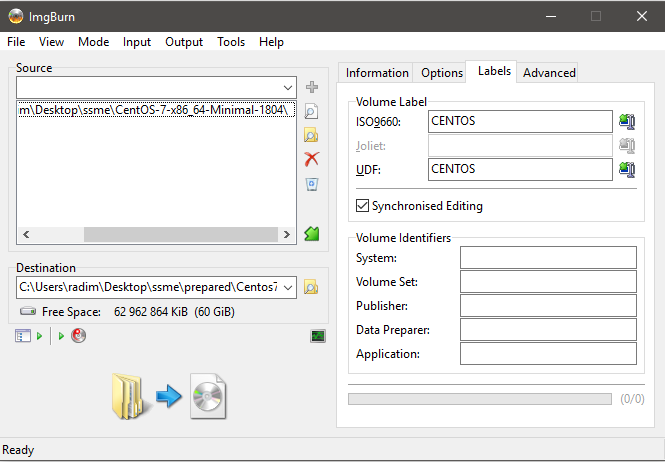
\includegraphics[trim={9.1cm 3cm 0.4cm 3cm},clip,width=.8\textwidth]{Screenshot_16.png}
    \caption{Volume label.}
    \label{pic:withoutresdrawable}
 \label{fig:sub1}\end{center}
\end{subfigure}%
\begin{subfigure}{.5\textwidth}
\begin{center}

 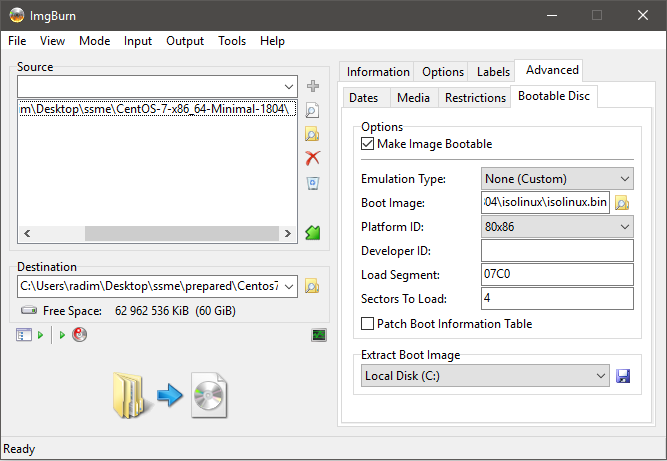
\includegraphics[trim={9.1cm 3cm 0.4cm 3cm},clip,width=.8\textwidth]{Screenshot_17.png}
    \caption{Boot image selection.}
\end{center}
\end{subfigure}
\label{fig:test}\caption{Ansible playbook and roles.}
\end{figure}


\subsubsection{Linux}
Once files are prepared, packaging into the iso at Linux is done by one-liner command:\\ \texttt{mkisofs -o centos7.iso -b isolinux.bin -c boot.cat \linebreak -no-emul-boot -V CENTOS -boot-load-size 4 -boot-info-table\linebreak -R -J -v -T isolinux/}.
    
%Installation to the target mining machine from this media can be done using optical media, USB drive that has the ISO unpackaged (e.g. using Rufus available from \url{rufus.ie}) or PXE boot (e.g. using open source network boot firmware iPXE available from \url{ipxe.org}).
    
\subsection{Setting up the OS using Ansible}
%Ansible is an IT automation engine that in this case is used for configuration and application management of local mining nodes. 
After installation from the ISO that was prepared with the kickstart file, the target machine is accepting SSH connections under root account using password-based authentification. Without proper configuration, this would leave machine open to brute force attempts for the root account.

Ansible uses following set of files to provision mining nodes with software and configuration:

\begin{figure}[H]
%\begin{subfigure}{.5\textwidth}
\dirtree{%
.1 /.
.2 xmr01.yml.
.2 hosts.
.2 ansible.cfg.
.2 roles/.
.3 ansible-sw-common-apps.
.3 ansible-sw-firewalld.
.3 ansible-sw-ntp.
.3 ansible-sw-postfix.
.3 ansible-sw-sshsec.
.3 ansible-sw-xmrstak.
.3 ansible-sys-hostname.
.3 ansible-user-add.
.3 ansible-yum-cron.
.3 ansible-yum-update.
}

  \label{fig:sub1}
  \caption{Ansible prepared roles.}
\end{figure}
%\begin{subfigure}{.5\textwidth}
\begin{itemize}
\itemsep0em
\item \texttt{Xmr01.yml} represents a playbook file that defines what group of nodes will be provisioned together with the list of roles that will be applied to them. \\
\texttt{Hosts} file contains groups of hosts with information on how Ansible can connect to them.
\item \texttt{Ansible.cfg} was used only in the testing environment where host key checking was disabled.
\item \texttt{Roles} folder contains roles that are applied when running the playbook.
\end{itemize}

\subsection{Ansible roles}
To make Linux mining nodes updated and secure, following roles were written:
\subsubsection{ansible-sw-common-apps}
The common baseline for all mining nodes that consists of the following tasks:
\begin{enumerate}
\itemsep0em
\item Ensure EPEL repo is configured or install it.
\item Install the following packages: \texttt{htop, rsync, screen, tmux, iftop, iotop, nano, git, wget, unzip, mc}.
\end{enumerate}
\subsubsection{ansible-sw-firewalld}
Installs and enables the firewalld service that has default policy for connections set to the \texttt{public network} and accepts incoming connections only for SSH service.
\subsubsection{ansible-sw-ntp}
To report correct information through the web interface of the mining software, the target machine has to be in sync with NTP servers to do that role establishes the following:
\begin{enumerate}
\itemsep0em
\item Package \texttt{ntpdate} installed from the CentOS repository.
\item Ensures correct timezone using \texttt{timedatectl} interface.
\item Creates daily cronjob for synchronization of system time.
\end{enumerate}
\subsubsection{ansible-sw-postfix}
Sets up email gateway for correct email delivery together with internal mail aliases mapped to a single outbound address. Email gateway can deliver email on its own to the recipient's server or can also act as a relay to Gmail account that is used for sending out emails. 

Using Gmail account is preferred as this solution is an Internet Service Provider (ISP) agnostic (blocked SMTP and SSMTP communication for outbound connections at the ISP level would be a problem for the gateway mode). 

Separate Gmail account for sending out email alerts is recommended as Postfix has login credentials saved in \texttt{/etc/postfix/sasl\linebreak\TextUnderscore{}passwd} file in plaintext \cite{van2015red}. This can be made more secure if the credentials file has appropriate permissions, e.g., ownership set to root, the group to wheel and chmod changed to 0600.

\subsubsection{ansible-sw-sshsec}
Takes care about incoming SSH connections in case somebody wants to try brute force attack on the mining machine. After a predefined amount of failed login attempts, the incoming IP address is put into "jail". 

Under the hood, fail2ban monitors sshd log for incoming failed attempts and after certain threshold creates a firewalld rule to block the IP for a predefined amount of time. The default setting for this rule is relatively strict, 3 failed attempts in 10-hour window result in a 10-hour ban for incoming connections from the IP address. 

This role is a fork of \texttt{ansible-role-fail2ban} that is available at \url{https://github.com/resmo/ansible-role-fail2ban}.

%TODO prolézt všechny role a zkontrolovat default vars
\subsubsection{ansible-sw-xmrstak}
Installs software collections \texttt{centos-release-scl} package for Centos together with \texttt{cmake3, devtoolset-4-gcc*, hwloc-devel, make, \newline libmicrohttpd-devel, openssl-devel} packages used for compiling XMR-Stak from source code.

After that, the folder structure inside the non-privileged user account is created, and XMR-Stak repo is cloned into the user directory. With appropriate permissions set, cmake compiles the source code with following flags: \texttt{cmake3 .. -DCPU\TextUnderscore{}ENABLE=ON -DCUDA\TextUnderscore{}ENABLE= OFF  -DOpen CL\TextUnderscore{}ENABLE=OFF} resulting in CPU only miner for Centos \cite{xmrstakcompile}.

If the mining node would use GPU, appropriate drivers from AMD or Nvidia website are a prior requirement for running the miner. As GPU feature is only a flag, it can be enabled on demand in the playbook file as cmake3 flags are set as variables in the tasks file of the \texttt{ansible-sw-xmrstak} role in the Jinja2 format: \\ \texttt{cmake3 .. -DCPU\TextUnderscore{}ENABLE=\{\{ DCPU\TextUnderscore{}ENABLE \}\} -DCUDA\TextUnderscore{}ENABLE=\{\{ \newline DCUDA\TextUnderscore{}ENABLE \}\} -DOpenCL\TextUnderscore{}ENABLE=\{\{ DOpenCL\TextUnderscore{}ENABLE \}\}}

As next step, role copies over to the node CPU, pool and miner configuration and creates a crontab entry for automatic miner start. For the final touch, HugePages are set to \texttt{vm.nr\TextUnderscore{}hugepages=128} in \texttt{/etc/sysctl.conf} for CPU mining memory allocation, and sysctl is reloaded.
\subsubsection{ansible-sys-hostname}
Changes system hostname to inventory hostname set in \texttt{hosts} file using \texttt{hostnamectl} Ansible module.
\subsubsection{ansible-user-add}
\texttt{User-add-role} is used for creating the mining user that is not within the wheel group (unprivileged user). 
\subsubsection{ansible-yum-cron}
Installs and configures automatic security updates for Centos that are daily checked against the online repository. If packages marked for security update are found, email notification to root is sent \cite{pelz2016centos}.
\subsubsection{ansible-yum-update}
All packages including kernel are updated so that mining node is ready to use and won't send update notification on the next day (unless there are new updates in the meantime).
\subsubsection{Additional notes}
Roles are installed in the order specified in the \texttt{xmr01.yml} file as system update is done as first to prevent any problems with XMR-Stak compilation. 

Using root account login on SSH is not recommended as the proper way would be to disable root login in \texttt{/etc/sshd\TextUnderscore{}config} and login to SSH using created non-privileged user account (ideally using ssh-key based authentification). 

Later if the user needs to login as user, this can be done by \texttt{su root} command. To minimize the chance of success brute force attack of the root account using SSH, fail2ban is set to strict mode. Although this is not the most secure way to access the system, with above settings this acts as a middle ground between security and usability of the mining operation.




%Ansible, Centos 7
\section{Windows-based solution}
\subsection{Installation media}
For Windows scenario, Windows 10 image from autumn 2018 was used. As installation is intended to run unattended, custom media has to be created.

There are many ways how to provision changes to original Windows media, most straightforward is generating an \texttt{autounattend.xml} file that covers all installation steps for Windows 10 installer.

This process of Windows image customization can be done using Windows Assessment and Deployment Kit (Windows ADK) as it includes Windows System Image Manager (Windows SIM) that is an authoring tool for \texttt{autounattend.xml} files. Using Windows ADK, more complex Windows deployment can be achieved as the administrator can bundle applications and drivers in the image \cite{rhodes2016introduction}.

For this guide, generating \texttt{autounattend.xml} file is based on online autounattend generator tool located at \url{windowsafg.com}. After generating the file, a block of commands that is executed after the first logon was added. 
\begin{figure}[H]
\begin{center}
\lstset{upquote=true}
\begin{lstlisting}
	<SynchronousCommand wcm:action=add>
   		<CommandLine>powershell -Command Set-ItemProperty -Path HKLM:\SOFTWARE\Wow6432Node\Microsoft\ .NetFramework\v4.0.30319 -Name SchUseStrongCrypto -Value 1 -Type DWord</CommandLine>
        <Description>Set PowerShell ExecutionPolicy</Description>
        <Order>42</Order>
        <RequiresUserInput>true</RequiresUserInput>
        </SynchronousCommand>
\end{lstlisting}
\caption{.NetFramework adjustments in the Autounattend file.}
    \label{fig:securecrypto}
\end{center}
    \end{figure} 
    \vspace{-2em}
For example, .NetFramework in Windows 10 doesn't have strong cryptography enabled for all .Net applications. Due to this, in the default state, Powershell can't be used for downloading updated code that is required for setting up the environment for Ansible. To fix that, one of the commands after the first logon is dedicated to this issue as shown in the Figure \ref{fig:securecrypto}.

After finishing the installation process and provisioning the Windows environment with \texttt{<FirstLogonCommands>} included in the unattended file, Ansible can connect to the Windows machine and set up thing properly. 

Note that installer opens RDP, WinRM, temporarily disables Windows Firewall (which will be properly configured by Ansible later) and sets up self-signed WinRM HTTPS certificate using Ansible Powershell file \texttt{ConfigureRemotingForAnsible.ps1} \cite{ansibleremoteps}. Mining node has to be connected to the network to download all required files properly.
\subsection{Ansible at Windows}
Before applying roles in Ansible for Windows, unlike in Ansible with Linux machines, environment for both Windows and Linux controller has to be prepared \cite{windowsansible}.
 
\textbf{Windows} needs to have WinRM setup. This is already done as it was part of the installation process where Ansible Powershell script set up HTTPS WinRM environment \cite{windowshostansible}.

\textbf{Linux} doesn't have Ansible modules for Windows in default Ansible install. Those can be installed using the package manager, e.g.:
\vspace{-0.7em}
\begin{itemize}
\itemsep0em
\item Ubuntu:
\begin{itemize}
\itemsep0em \vspace{-0.7em}
\item Python 2: apt-get install python-winrm
\item Python 3: apt-get install python3-winrm
\end{itemize}
\item Centos:
\begin{itemize}
\itemsep0em \vspace{-0.7em}
\item With EPEL enabled: yum install python2-winrm
\end{itemize}
\item Or using PIP:
\begin{itemize}
\itemsep0em  \vspace{-0.7em}
\item pip install pywinrm
\end{itemize}
\end{itemize}

\subsection{Ansible roles}
Once Ansible is ready to launch \texttt{xmratwin.yml} playbook, the following roles are played:
\begin{figure}[H]
%\begin{subfigure}{.5\textwidth}
\dirtree{%
.1 /.
.2 xmratwin.yml.
.2 hosts.
.2 ansible.cfg.
.2 roles/.
.3 ansible-win-sec.
.3 ansible-win-updates.
.3 ansible-win-xmrstak.
}

  \label{fig:sub1}
  \caption{Ansible roles for Windows.}
\end{figure}
\subsubsection{ansible-win-sec}
Sets up firewall rules for RDP, WinRM and XMR-Stak web interface, enables Windows firewall for all zones.
\subsubsection{ansible-win-updates}
Windows update policy is set to download and notify for install as Windows updates are managed by this Ansible role. 

The administrator can configure which updates category will be included in the updates, in default role install updates from \texttt{SecurityUpdates} and \texttt{CriticalUpdates} category \cite{windowshostansible}. This can be changed using variable \texttt{UpdateEverything} in the playbook.
\subsubsection{ansible-win-xmrstak}
Downloads latest release of XMR-Stak from developers GitHub page, configures mining software and downloads required libraries from Microsoft site. It also creates scheduled task under the mining user to run with elevated permissions after login so that UAC can be kept enabled and the miner is running without UAC prompts. 

Also adds the exception in Windows Defender to ignore Desktop folder as a binary XMR-Stak file is considered as a malicious file for being a mining software.

\chapter{Conclusion}
Monero cryptocurrency is a large and active project that offers a wide range of applications for both users and miners. For its open-source nature, everyone can build own wallet software, miner or even a website that provides wallet and key management. Because of this, many good, but also potentially malicious applications are released to the public. 

The goal of this thesis is to map usage habits of Monero cryptocurrency users and miners from both technological as well as security view. Another goal is to create a detailed user guideline for user-friendly and secure usage of the Monero cryptocurrency including key management and backup strategy. For miners, the goal is to implement an automated deployment of mining rigs using one of the popular configuration management tools.

To address this issue, thesis provides detailed overview of Monero environment, comparison of wallet client software and exchanges, comparison of mining software and list of malicious events and software connected with Monero cryptocurrency.

For deeper investigation of the listed issues, I have conducted surveys aimed at Monero users and miners. With 173 (113 in users and 60 in miners survey) respondents in total, this provides a real Monero users sample upon which two guidelines were proposed. %First for secure usage of Monero cryptocurrency and for .

Results of Monero User Research follow the way how participants were selected (by self-selection) as well as the sites they came from (Reddit, Facebook cryptocurrency groups). That meant that majority of users said they prefer Linux OS with official wallet software and also that they tend to use open-source more then closed-source software. Only a few of them used closed-source apps or website portals that can be labeled as dangerous for the user. Contrary to popular belief, respondents revealed that they use Monero for darknet markets only in 18\% (20 out of 113), in case of drugs in 10\% (11 out of 113) and for other illegal usecases in 5\% (6 out of 113).

Based on the results of the research, I formulated Monero usage and storage best practices part of the thesis, which gives users detailed steps on how to work with the Monero cryptocurrency.

Monero Miners Research revealed that both Windows and Linux mining operations are set up using manual deployment and updates are usually disabled or delayed. Mining software was in almost all cases open-source with XMR Stak being used the most. 

Based on the results from the Monero Miners Research, I implemented an automated deployment system for both major platforms using unattended/kickstart installation media and Ansible. By using application deployment and configuration management tool like Ansible, miners are able to deploy large mining operations with correct security settings that are both secure and easy to maintain. 

As for the future work on this topic, it would be appropriate to extend current research to include other cryptocurrencies (Dash, Ethereum or Bitcoin) as well as deployment of their miners. 

To make results from this thesis more open to the public, everything is published under the GitHub repository and GitHub pages website. Website links are avaiable in the Appendix Figure \ref{cha:listofattachments}.

%na zaklade motivace jsem delal toto, výsledky byly tyto, zjisteni vyzkumu users, miners a nazaklade jejich jsem udelal implementaci co se tyce future work vidim jako mozna budouci pole půsovnosti tohleto tamhleto.




\iffalse There is a thin line between reasonable security and unnecessary security measures that render the whole work useless. More often than not, systems, applications, and whole environments are designed with security in mind, but without the idea how to do it in a usable way, resulting in user-created workarounds that cause security issues.

In Monero cryptocurrency, there are no strict guidelines or rules on how to access the funds or run the mining operation. As can be seen on the results from both of the surveys, users tend to only "do the needful" when it comes to using the cryptocurrency.

%Monero cryptocurrency is an active open source technology project that aims to provide private cryptocurrency for everyone. As there is no central authority it is always up to the community to recommend or guide others 

In terms of security in mining operations as well as normal users key management there is a room for improvement. Using the combination of knowledge from  Monero documentation, Monero community articles, and posts as well as results from both of the surveys and own technological background, this work presents a detailed view on the technical side of the cryptocurrency.

User side of Monero is represented by the description of the cryptocurrency as well as detailed guidelines on how to start with the cryptocurrency in form of best practices. This includes choosing the client software, deciding on the type the wallet, generating and storing the keys up to pointing out the problems and incidents that can happen to every user.

This work can further be extended by covering the pool operators perspective,  system management, and security standards. At the time of writing, there was not enough data to dig into this section as none out of more than 20 pools filled out the survey.

From miners perspective, the thesis offers the guide on how to automate deployment and configuration of mining operations. This is important as only a small fraction from both Windows and Linux miners use automation tools to deploy and manage mining rigs which can result in unwanted differences in configuration or inconsistencies across mining environment.

To make results from this thesis more open to the public, everything is published under the GitHub repository and GitHub pages website. Website links are avaiable in the Appendix Figure \ref{cha:listofattachments}.
%\noindent
%GitHub repository: \url{https://github.com/Ownercz/ssme-thesis}\\
%GitHub pages: \url{https://ownercz.github.io/ssme-thesis}

\fi

\setlength{\emergencystretch}{3em}
\printbibliography[heading=bibintoc]
\let\cleardoublepage\clearpage
\begingroup
\let\cleardoublepage\clearpage
\appendix
\chapter{List of Attachments}
\label{cha:listofattachments}
Electronic attachments are included in the thesis archive of the Masaryk University Information System. 
\\
\\
Thesis source code together with electronic attachments is available at \url{https://github.com/Ownercz/ssme-thesis}. 
\\
\\
Chapters of this work are also published online at \url{https://ownercz.github.io/ssme-thesis/}. 
\\
\\
Following files are included in the attachment archive:
\begin{itemize}
\itemsep0em
\item \texttt{Ansible} directory containing Ansible playbook and roles for Linux and Windows miner deployment.
\item \texttt{Cleansed} directory containing data used for Monero Users and Monero Miners survey.
\item \texttt{Kickstart} directory containing the kickstart file for Centos 7 used in unattended Centos installation.
\item \texttt{Original} directory containing unfiltered data from Monero Users and Monero Miners survey.
\item \texttt{SQL-queries} directory containing SQL files that were used for data processing for both surveys.
\item \texttt{Unattended} directory containing the autounattend file for Windows 10 used in unattended Windows 10 installation.
\end{itemize}


\chapter{Responses Sorted by Country -- User Research}
\vspace{-1em}
\begin{figure}[H]
\center
\begin{footnotesize}
\begin{tabular}{ccl}
\textbf{Number of responses} & \textbf{Country shortcode} & \textbf{Country name} \\
31 & US & United States      \\
17 & CZ & Czech Republic     \\
11 & DE & Germany            \\
03  & CA & Canada             \\
03  & SK & Slovakia           \\
03  & GB & United Kingdom     \\
04  & BE & Belgium            \\
03  & RU & Russian Federation \\
03  & NL & Netherlands        \\
02  & SI & Slovenia           \\
02  & HK & Hong Kong          \\
02  & FR & France             \\
02  & FI & Finland            \\
02  & BR & Brazil             \\
02  & BG & Bulgaria           \\
02  & AU & Australia          \\
01  & UA & Ukraine            \\
01  & TR & Turkey             \\
01  & RS & Serbia             \\
01  & RO & Romania            \\
01  & PT & Portugal           \\
01  & PL & Poland             \\
01  & PH & Philippines        \\
01  & NO & Norway             \\
01  & MY & Malaysia           \\
01  & MU & Mauritius          \\
01  & IT & Italy              \\
01  & GR & Greece             \\
01  & ES & Spain              \\
01  & AF & Afghanistan       
\end{tabular}
\end{footnotesize}
\caption{Responses by country in user research.}
\label{table:countries}
\end{figure}


\chapter{Responses Sorted by Country -- Miners Research}
\vspace{-2em}
\begin{figure}[H]
\center
\begin{tabular}{ccl}
\textbf{Number of responses} & \textbf{Country shortcode} & \textbf{Country name} \\
10                           & US                         & United States         \\
10                           & CZ                         & Czech Republic        \\
06                            & DE                         & Germany               \\
03                            & RU                         & Russian Federation    \\
03                            & PT                         & Portugal              \\
03                            & CA                         & Canada                \\
02                            & RO                         & Romania               \\
02                            & PL                         & Poland                \\
02                            & NO                         & Norway                \\
02                            & NL                         & Netherlands           \\
02                            & HK                         & Hong Kong             \\
02                            & BG                         & Bulgaria              \\
01                            & ZA                         & South Africa          \\
01                            & SK                         & Slovakia              \\
01                            & SE                         & Sweden                \\
01                            & MY                         & Malaysia              \\
01                            & LR                         & Liberia               \\
01                            & IT                         & Italy                 \\
01                            & GR                         & Greece                \\
01                            & GB                         & United Kingdom        \\
01                            & FR                         & France                \\
01                            & DK                         & Denmark               \\
01                            & BR                         & Brazil                \\
01                            & AU                         & Australia             \\
01                            & AF                         & Afghanistan           \\
\end{tabular}
\caption{Responses by country in miners research.}
\label{table:countriesminers}
\end{figure}

\includepdf[pages=1,pagecommand=\chapter{Monero User Survey},scale=1.1,width=1.1\textwidth]{monerousersurvey.pdf}
\label{monero-user-study-pdf}
\includepdf[pages={2,3,4,5,6,7,8,9},scale=1,width=1.1\textwidth, pagecommand={}]{monerousersurvey.pdf}
\includepdf[pages=1,pagecommand=\chapter{Monero Miners Survey},scale=1,width=1.1\textwidth]{monerominersurvey.pdf}
\label{monero-miners-study-pdf}
\includepdf[pages={2,3,4,5,6,7,8,9},scale=1,width=\textwidth, pagecommand={}]{monerominersurvey.pdf}
%\includepdf[pages=1,pagecommand=\chapter{Monero User Survey},scale=0.7]{moneropoolsurvey.pdf}
%\label{monero-pool-study-pdf}
%\includepdf[pages={2,3,4,5},scale=0.7, pagecommand={}]{moneropoolsurvey.pdf}

\chapter{Kickstart file}
\label{kickstart}
\begin{lstlisting}
#version=DEVEL
# System authorization information
auth --enableshadow --passalgo=sha512
# Use network installation
url --url=http://ftp.fi.muni.cz/pub/linux/centos/7/os/x86_64/
repo --name=base --baseurl=http://ftp.fi.muni.cz/pub/linux/centos/7/os/x86_64/
# Use graphical install
graphical
# Run the Setup Agent on first boot
firstboot --enable
ignoredisk --only-use=sda
# Keyboard layouts
keyboard --vckeymap=us --xlayouts=us
# System language
lang en_US.UTF-8

# Network information
network  --bootproto=dhcp --device=ens192 --ipv6=auto --activate
network  --bootproto=dhcp --hostname=changeme.lipovcan.cz
# Reboot after installation
reboot
# Root password
rootpw --iscrypted $6$jtf4WZQD/5Ozocag$5UcoItitnW58zDBA3k.itRf7ozUA391
# System services
services --enabled=chronyd
# System timezone
timezone Europe/Prague --isUtc --ntpservers=tik.cesnet.cz
# System bootloader configuration
bootloader --append= crashkernel=auto --location=mbr --boot-drive=sda
autopart --type=lvm
# Clear the Master Boot Record
zerombr
# Partition clearing information
clearpart --all --initlabel
\end{lstlisting}
\newpage
\begin{figure}[H]
\begin{lstlisting}
%packages
@^minimal
@core
chrony
kexec-tools
kexec-tools

%end

%addon com_redhat_kdump --enable --reserve-mb=auto

%end

%anaconda
pwpolicy root --minlen=6 --minquality=50 --notstrict --nochanges --notempty
pwpolicy user --minlen=6 --minquality=50 --notstrict --nochanges --notempty
pwpolicy luks --minlen=6 --minquality=50 --notstrict --nochanges --notempty
%end
\end{lstlisting}


\center
\caption{Centos 7 kickstart file.}
\label{fig:kickstart}
\end{figure}
\chapter{Automated installation process}
In order to show automated installation process for both Windows and Linux miners, both installation processes were recorded using HDMI capture card and Open Broadcaster Software (OBS). Timeline detailing installation process is avaiable in the Figures \ref{windows-timeline} and \ref{linux-timeline}.

Video is avaiable at \url{https://github.com/Ownercz/ssme-thesis/blob/master/video.md} .

\begin{figure}[H]
\color{gray}
\rule{\linewidth}{1pt}
\ytl{00:20}{Start of unattended Windows installation using the autounattend file}
\ytl{05:35}{Install part complete, OS first boot}
\ytl{11:07}{Windows 10 installation complete}
\ytl{11:15}{Running Ansible playbook on the Windows machine}
\ytl{13:38}{Ansible completes miner deployment and reboots the machine}
\ytl{15:17}{Ansible sets up firewall, Windows environment and reboots the machine. Miner is already running because of scheduled task after reboot}
\ytl{17:18}{Ansible updates the OS using Windows update module}
\ytl{55:24}{Ansible reboots the machine to complete the updates}
\ytl{57:25}{Ansible completes the playbook and mining machine is ready}
\bigskip
\rule{\linewidth}{1pt}%
\color{black}
\caption{Automated deployment of Windows mining machine.}
\label{windows-timeline}
\end{figure}
\pagebreak




\begin{figure}[H]
\begin{centering}
 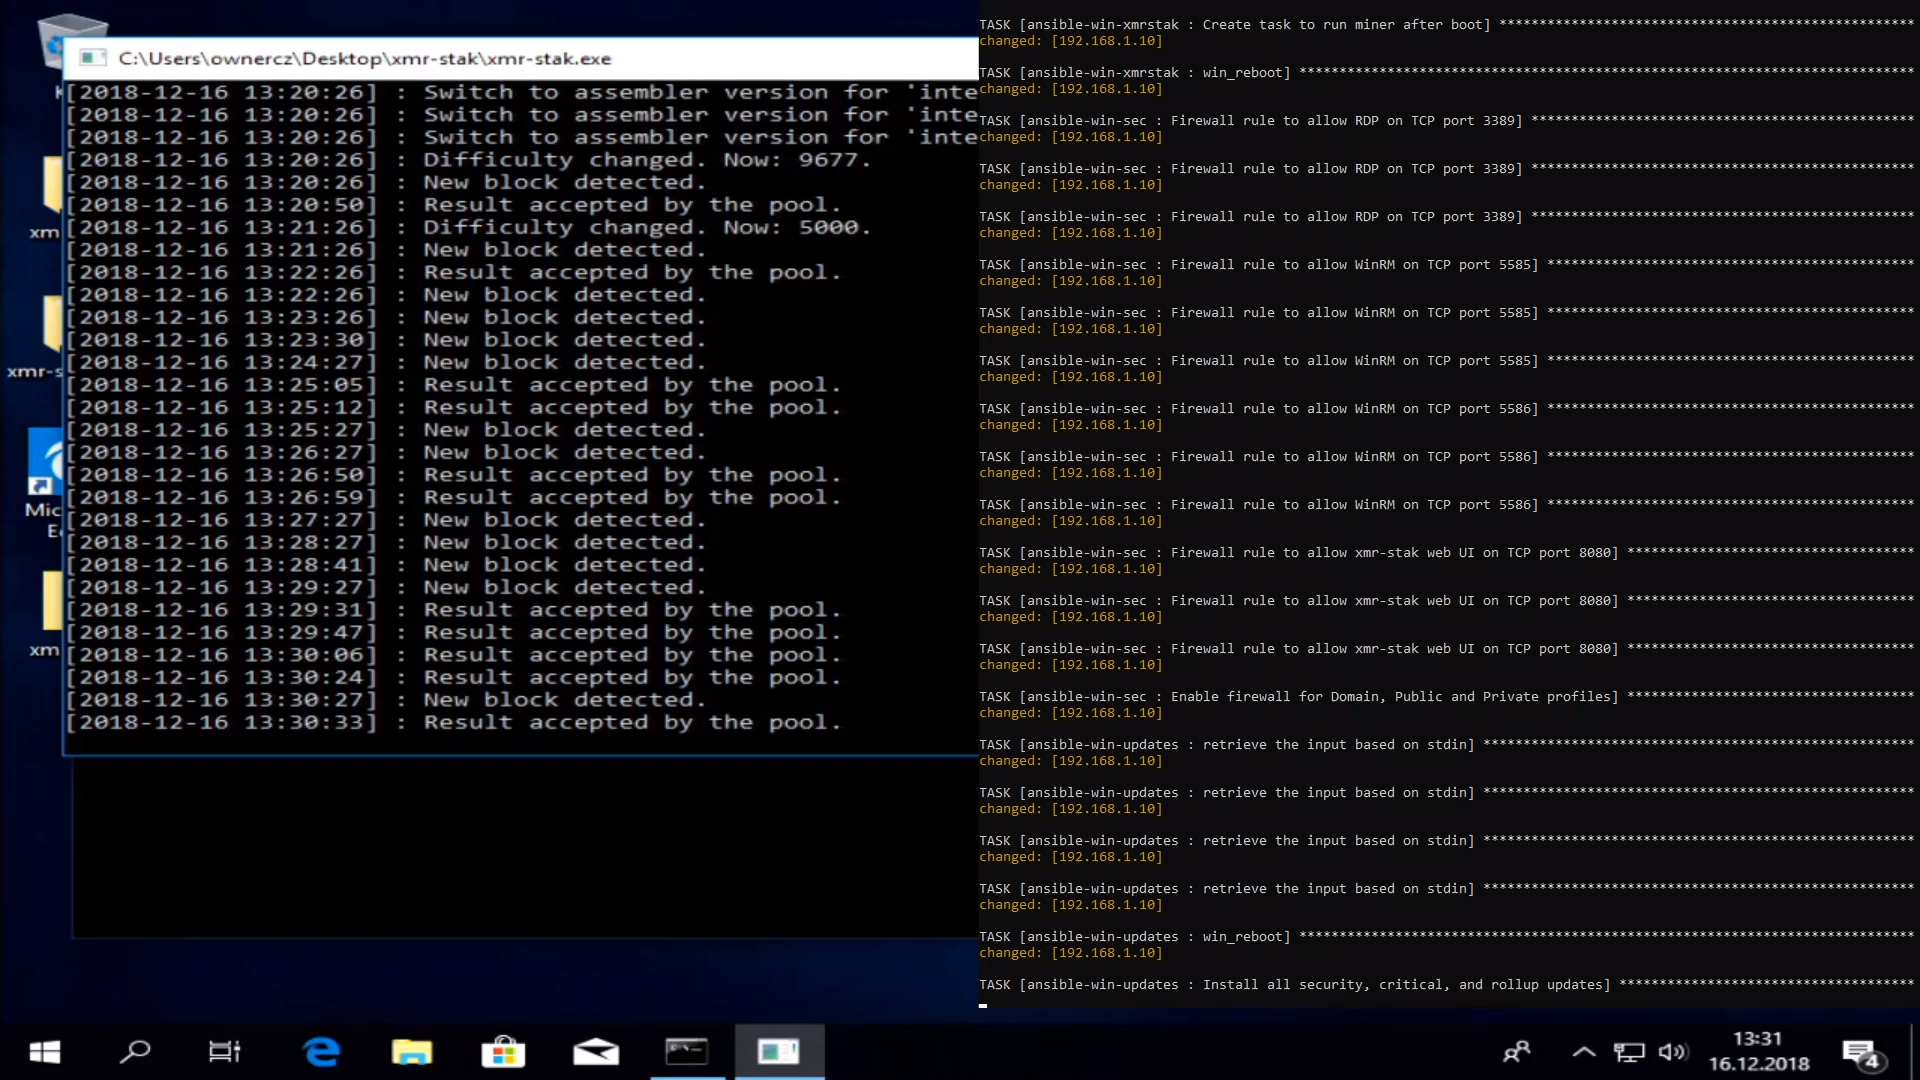
\includegraphics[trim={0 0 0 0},clip,width=0.95\textwidth]{Screenshot_20190303_105607.png}
  \caption{Windows miner deployment.}
    \label{pic:windows-mining}
\end{centering}
    \end{figure}

Both installations were done using USB drive as installation source. Hardware specifications of the installation computer were CPU Intel i5 4460, 24GB of DDR3 RAM and target installation drive was 60GB Intel 330 SATA SSD.

\begin{figure}[H]
\color{gray}
\rule{\linewidth}{1pt}
\ytl{00:46}{Start of unattended Linux Centos 7 installation using the kickstart file}
\ytl{05:06}{Install part complete, OS first boot}
\ytl{05:06}{Running Ansible playbook on the Linux machine}
\ytl{11:29}{Ansible completes the playbook and mining machine is ready}
\bigskip
\rule{\linewidth}{1pt}%
\color{black}
\caption{Automated deployment of Linux mining machine.}
\label{linux-timeline}
\end{figure}


 %% Start the appendices.
%\chapter{Zdroje k tabulce 2.2}
%dash https://bitcointalk.org/index.php?topic=1562109.0
%dash https://docs.dash.org/en/latest/introduction/information.html
%pivx https://github.com/PIVX-Project/PIVX
%pivx https://www.reddit.com/r/pivx/comments/7gjjyw/what_are_the_benefits_of_multisig_addresses/
%zcoin https://github.com/zcoinofficial/zcoin/wiki/Information-for-exchanges
%zcoin https://zcoin.io/zcoins-privacy-technology-compares-competition/
\endgroup
\end{document}
